%%%%%%%%%%%%%%%%%%%%%%%% editor.tex %%%%%%%%%%%%%%%%%%%%%%%%%%%%%
%
% sample root file for the contributions of a "contributed volume"
%
% Use this file as a template for your own input.
%
%%%%%%%%%%%%%%%%%%%%%%%%%%%%% Springer %%%%%%%%%%%%%%%%%%%%%%%%%%


% RECOMMENDED %%%%%%%%%%%%%%%%%%%%%%%%%%%%%%%%%%%%%%%%%%%%%%%%%%%
\documentclass[graybox, envcountchap, natbib]{svmult}

% choose options for [] as required from the list
% in the Reference Guide

%\usepackage{type1cm}        % activate if the above 3 fonts are 
                             % not available on your system

\usepackage{makeidx}         % allows index generation
\usepackage{graphicx}        % standard LaTeX graphics tool
                             % when including figure files
\usepackage{multicol}        % used for the two-column index
\usepackage[bottom]{footmisc}% places footnotes at page bottom

\usepackage{newtxtext}       % 
\usepackage{newtxmath}       % selects Times Roman as basic font
\usepackage{doi}             % makes hyperlinks out of doi in bib

\usepackage{kantlipsum}
\usepackage{wrapfig}

\let\Bbbk\relax              % MER: Fixes compilation error

% see the list of further useful packages in the Reference Guide
\usepackage{chapterbib}
\input{packages}
\input{commands}
\input{macros}
\makeindex             % used for the subject index
                       % please use the style svind.ist with
                       % your makeindex program

                       
\usepackage{cleveref} % Load cleverref after packages to support algorithm

\crefname{chapter}{Chap.}{Chaps}
\Crefname{chapter}{Chapter}{Chapters}
\crefname{section}{Sect.}{Sects.}
\Crefname{section}{Section}{Sections}
\crefname{figure}{Fig.}{Figs.}
\Crefname{figure}{Figure}{Figures}
\crefname{table}{Table}{Tables}
\Crefname{table}{Table}{Tables}
\crefname{volume}{Vol.}{Vols.}
\Crefname{volume}{Volume}{Volumes}
\crefname{equation}{}{}
\Crefname{equation}{Equation}{Equations}
\crefname{algorithm}{Alg.}{Algs.}
\Crefname{algorithm}{Algorithm}{Algorithms}
\crefname{definition}{Def.}{Defs.}
\Crefname{definition}{Definition}{Definitions}
\crefname{listing}{code listing}{code listings}
\Crefname{listing}{Code Listing}{Code Listings}

%%%%%%%%%%%%%%%%%%%%%%%%%%%%%%%%%%%%%%%%%%%%%%%%%%%%%%%%%%%%%%%%%

\begin{document}

\frontmatter%%%%%%%%%%%%%%%%%%%%%%%%%%%%%%%%%%%%%%%%%%%%%%%%%%%%%%

\include{dedication}
%%%%%%%%%%%%%%%%%%%%%%foreword.tex%%%%%%%%%%%%%%%%%%%%%%%%%%%
% sample foreword
%
% Use this file as a template for your own input.
%
%%%%%%%%%%%%%%%%%%%%%%%% Springer %%%%%%%%%%%%%%%%%%%%%%%%%%

\foreword

%% Use the template \textit{foreword.tex} together with the document class SVMono (monograph-type books) or SVMult (edited books) to style your foreword\index{foreword}. 

%% The foreword covers introductory remarks preceding the text of a book that are written by a \textit{person other than the author or editor} of the book. If applicable, the foreword precedes the preface which is written by the author or editor of the book.

This book provides highlights of the research presented at
the FEniCS 24 meeting held in Oslo, Norway in June, 2024.
The selected topics published here show the typical breadth of FEniCS research as a whole,
including
\begin{itemize}
\item
new software and algorithm developments, including some performance assessment
of the implementations
on advanced computer architectures, and
\item
computational simulation of challenging applications using some version of FEniCS (dolfin).
\end{itemize}
This book not only confirms the original objectives of the FEniCS Project,
but it also demonstrates the continuing vitality of the the original concepts
behind the FEniCS Project.

The FEniCS Project was started at an informal meeting at the
University of Chicago in 2003. It has grown to an international
collaboration involving primary developers and users at sites in England, 
Europe, Asia, and the Americas. 
Discounting the Covid era, the FEniCS Project has held an annual, 
in-person meeting
at sites in England, Europe, and the United States, often including tutorial
sessions on ``how to use it'' for beginners.
The online FEniCS meeting during the Covid era utilized some special software
that enabled and encouraged personal contact with people you had never met before.
I have had the pleasure to attend almost all of the FEniCS meetings, with
just a few exceptions.
This book is the first refereed conference proceedings for the FEniCS meetings.

FEniCS was one of the first projects to address the automation 
of computational mathematical modeling \cite{lrsBIBih}.
This includes tools to generate key components of 
scientific simulation software as well as complete end-user 
systems based on these tools. The end-user codes are being 
used to solve challenging problems in fluid dynamics, heat 
transfer, advanced materials, and many other areas, including 
what is now known as multiphysics.
Novice users at remote sites 
have been able to assemble codes for complex simulations 
using novel models with little help from developers.
Initially, such help came primarily via e-mail, but today
online systems such as 
{\tt https://fenicsproject.discourse.group}
are used.

One feature of FEniCS was that it encouraged publication of the
algorithms behind the software.
This provided academic recognition that is missing from some
other software projects.
This approach was copied from computer science, where it is standard.
There are long-standing journals in which early FEniCS research
was published.
More recently, journals devoted to scientific software have emerged.
Thus, FEniCS pioneered a culture shift regarding how software is 
viewed and documented.

FEniCS has, since its inception, involved various bifurcations
as people developed different end-user interfaces and internal
software implementations to achieve different targeted objectives.
One such bifurcation involved the development of a high-performance
(highly parallel) version, while the main branch targeted a broader
user interface and internal structure to attract a larger user base.
A later bifurcation led to the Firedrake project.
Thus, the FEniCS Project has provided an environment in which different
approaches were able to flourish, and this feature continues today,
despite the fact that legacy FEniCS software is still widely used.

FEniCS (and Firedrake and others) rely on the variational formulation of 
partial differential equations (PDEs) to provide a language to express
simulation models.
This possibility was recognized already in the first edition of the book
~\cite{lrsBIBcq} (see the end of the first paragraph in Chapter 0).
This observation was, a decade later, demonstrated in the system
Analysa~\cite{lrsBIBfo}.
A different approach to a language for PDEs appeared earlier in the
finite difference language FIDIL~\cite{hilfinger1989fidil}.

NGSolve uses syntax similar to that of FEniCS and Firedrake, so that
codes written for one system are easy to port to another.
One valuable aspect of FEniCS and other projects is that they allow
algorithm developers a way to make their advances available to
a wide audience.
A code written from scratch is hard to use by novices, and such
codes often are underutilized.

Analysa~\cite{lrsBIBfo} provided only a limited family of elements,
but arbitrary order Lagrange elements were available, generated
automatically by a specific algorithm.
One feature of Analysa that is not yet replicated in FEniCS (or Firedrake)
is an algebra of domains and corresponding finite element spaces.
It was possible in Analysa to define a space of functions on the boundary,
on the interior, and to define linear functionals and matrices
related to these spaces.
This provided a way to implement the linear algebra for problem
solution precisely.
Perhaps such functionality can appear in future automated PDE software.


FEniCS has allowed the development and testing of new ideas by a
very large community, including people with minimal software training.
Often a new technique can be tested numerically before expending
the effort to understand the new method analytically.
For example, the Robin method described in \cite{lrsBIBig} was first
tested on a simple problem before attempting to show that the method
was well posed.
In fact, the proof of that took significant time, since it required
discovering a new approach to analyzing finite element methods.
Without the assurance that the method actually worked in practice,
we likely would have abandoned the search for a rigorous explanation
of its behavior.

Today users have many options to choose from when approaching the 
implementation of a technical model.
This includes Firedrake, NGSolve, and various flavors of FEniCS.
The legacy version of FEniCS (dolfin) from 2019 is still widely used.
This is not the forum to compare and contrast these different choices,
but one can find some guidance from online discussions.

The current volume gives a glimpse of the leading edge
of FEniCS-related research.
It is a good way to find out current research topics and get a sense
of directions for the FEniCS Project for the future.

Ridgway Scott was one
of the founders of FEniCS, and Matt Knepley (of the Computation
Institute) has become one of the major developers. Two
graduate students in CS are also primary developers. Current
efforts are underway to extend FEniCS from traditional two- and 
three-dimensional models in mechanics to arbitrary dimensional 
systems as arise in quantum mechanics. FEniCS has also hosted
conferences that feature automated scientific software
development outside its primary domain of solving partial
differential equations.




\vspace{\baselineskip}
\begin{flushright}\noindent
Chicago, USA, 22nd October 2025\hfill {\it L. Ridgway Scott}\\
\end{flushright}



\bibliography{histor}
%\bibliographystyle{IEEEtran}
\bibliographystyle{plainnat}
%\bibliographystyle{unsrtnat}

%%%%%%%%%%%%%%%%%%%%%%preface.tex%%%%%%%%%%%%%%%%%%%%%%%%%%%%%%%%%%%%%%%%%
% sample preface
%
% Use this file as a template for your own input.
%
%%%%%%%%%%%%%%%%%%%%%%%% Springer %%%%%%%%%%%%%%%%%%%%%%%%%%

\preface

TODO

\vspace{\baselineskip}
\begin{flushright}\noindent
Oslo, Norway, 22nd October 2025
\hfill{\it Jørgen S.\ Dokken, Henrik N.\ T.\ Finsberg, Jack S.\ Hale, Marie E.\ Rognes, Matthew W. Scroggs}\\
\end{flushright}

\include{acknowledgement}

\setcounter{tocdepth}{0}
\tableofcontents
\include{contriblist}
\include{acronym}

\mainmatter%%%%%%%%%%%%%%%%%%%%%%%%%%%%%%%%%%%%%%%%%%%%%%%%%%%%%%%

% Document commands
% --- Auxiliary functions ---

% --- Settinge ---
\newcommand{\bracketed}[1]{\left[#1\right]}

% --- General ---
% Absolute value
\NewDocumentCommand{\abs}{m}{
    % #1: argument
    \left\vert#1\right\vert
}

% --- Linear Algebra ---
% Inner product
\NewDocumentCommand{\iprod}{o m m}{
    % #1: the domain (for integration)
    % #2: argument 1
    % #3: argument 2
    \left(#2,\: #3\right)\IfValueT{#1}{_{#1}}
}

\NewDocumentCommand{\iprodS}{o m m}{
    % #1: the domain (for integration)
    % #2: argument 1
    % #3: argument 2
    \left\langle#2,\: #3\right\rangle\IfValueT{#1}{_{#1}}
}

% Norm
\NewDocumentCommand{\norm}{o m}{
    % #1: Specifier of the norm
    % #2: argument
    \left\vert\left\vert#2\right\vert\right\vert\IfValueT{#1}{_{#1}}
}

% --- Basic tensor functions
% Transposition
\NewDocumentCommand{\transpT}{o m}{
    % #1: Indices of the transposition
    % #2: The tensor
    #2\IfNoValueTF{#1}{^\mathrm{T}}{^{\overset{#1}{\mathrm{T}}}}
}

% % The trace
% \NewDocumentCommand{\tr}{o m}{
%     % #1: True, if brackets should be used
%     % #2: The tensor
%     \mathrm{tr}\IfNoValueTF{#1}{\: #2}{\bracketed{#2}}
% }

% Additive decomposition
\NewDocumentCommand{\sym}{o m}{
    % #1: True, if brackets should be used
    % #2: The tensor
    \mathrm{sym}\IfNoValueTF{#1}{\: #2}{\bracketed{#2}}
}

\NewDocumentCommand{\skw}{o m}{
    % #1: True, if brackets should be used
    % #2: The tensor
    \mathrm{skw}\IfNoValueTF{#1}{\: #2}{\bracketed{#2}}
}

% \NewDocumentCommand{\as}{o m}{
%     % #1: True, if brackets should be used
%     % #2: The tensor
%     \mathrm{as}\IfNoValueTF{#1}{\: #2}{\bracketed{#2}}
% }

% Determinant
\NewDocumentCommand{\determ}{o m}{
    % #1: True, if brackets should be used
    % #2: The tensor
    \mathrm{det}\IfNoValueTF{#1}{\: #2}{\bracketed{#2}}
}

% Inverse
\NewDocumentCommand{\inv}{o m}{
    % #1: True, if brackets should be used
    % #2: The tensor
    \IfNoValueTF{#1}{#2 ^{-1}}{\bracketed{#2}^{-1}}
}

\NewDocumentCommand{\invt}{o m}{
    % #1: True, if brackets should be used
    % #2: The tensor
    \IfNoValueTF{#1}{#2 ^{-\mathrm{T}}}{\bracketed{#2}^{-\mathrm{T}}}
}

% --- Analysis ---
% Gradient and Divergence 
\newcommand{\grad}{\nabla\:}
\renewcommand{\div}{\nabla\cdot}

\NewDocumentCommand{\divc}{o m m}{
    % #1: True, if brackets should be used
    % #2: The arguemnt
    % #3: Configuration, within which the divergence is evaluated
    \nabla_{\vec{#3}} \cdot \IfNoValueTF{#1}{#2}{\bracketed{#2}}
}

\NewDocumentCommand{\gradc}{o m m}{
    % #1: True, if brackets should be used
    % #2: The arguemnt
    % #3: Configuration, within which the divergence is evaluated
    \nabla_{\vec{#3}} \: \IfNoValueTF{#1}{#2}{\bracketed{#2}}
}

% Integrational domains
\newcommand{\dInt}[1]{\;\mathrm{d}#1}
\newcommand{\dVol}{\;\mathrm{d}v}
\newcommand{\dVolR}{\;\mathrm{d}V}
\newcommand{\dSurf}{\;\mathrm{d}a}
\newcommand{\dSurfR}{\;\mathrm{d}A}

% Material timederivative
\NewDocumentCommand{\mtDiff}{o m}{
    % #1: True, if brackets should be used
    % #2: The arguemnt
    \IfNoValueTF{#1}{#2'}{\left(#2\right)'}
}

% Gateaux derivative
\newcommand{\dGat}[2]{\mathrm{D}_{#2}\left[#1\right]}

% Linearisation
\newcommand{\Lin}[1]{\mathrm{LIN}\left[#1\right]}

% --- Function spaces ---
\NewDocumentCommand{\VecSpace}{o o o m}{
    % #1: The domain
    % #2: The boundary condition
    % #3: The dimension
    % #4: The function-space
    \IfNoValueTF{#3}
    {\mathrm{#4} \IfValueT{#2}{_{#2}} \ifthenelse{\equal{#1}{}}{}{\left(#1\right)}}
    {\left( \mathrm{#4} \IfValueT{#2}{_{#2}} \ifthenelse{\equal{#1}{}}{}{\left(#1\right)} \right) ^{#3}}
}

\NewDocumentCommand{\LiiSpace}{o o o}{
    % #1: The domain
    % #2: The boundary condition
    % #3: The dimension
    \IfNoValueTF{#3}
    {\mathrm{L}^2 \IfValueT{#2}{_{#2}} \ifthenelse{\equal{#1}{}}{}{\left(#1\right)}}
    {\left( \mathrm{L}^2 \IfValueT{#2}{_{#2}} \ifthenelse{\equal{#1}{}}{}{\left(#1\right)} \right) ^{#3}}
}

\NewDocumentCommand{\HiSpace}{o o o}{
    % #1: The domain
    % #2: The boundary condition
    % #3: The dimension
    \IfNoValueTF{#3}
    {\mathrm{H}^1 \IfValueT{#2}{_{#2}} \IfValueT{#1}{\left(#1\right)}}
    {\left( \mathrm{H}^1 \IfValueT{#2}{_{#2}}\IfValueT{#1}{\left(#1\right)} \right) ^{#3}}
}

\NewDocumentCommand{\HdivSpace}{o o o}{
    % #1: The domain
    % #2: The boundary condition
    % #3: The dimension
    \IfNoValueTF{#3}
    {\mathrm{H} \IfValueT{#2}{_{#2}} \left(\mathrm{div}\ifthenelse{\equal{#1}{}}{}{,\, #1}\right)}
    {\left( \mathrm{H} \IfValueT{#2}{_{#2}} \left(\mathrm{div}\ifthenelse{\equal{#1}{}}{}{,\, #1}\right) \right) ^{#3}}
}

% --- Finite element spaces ---
\NewDocumentCommand{\sdisc}{m}{
    % #1: The field variable
    #1_{\h}
}

\NewDocumentCommand{\stdisc}{m}{
    % #1: The field variable
    #1_{\h\tau}
}

\NewDocumentCommand{\feP}{o o}{
    % #1: The degree
    % #2: The dimension
    \IfNoValueTF{#2}
    {\mathrm{P} \IfValueT{#1}{_{#1}}}
    {\left( \mathrm{P} \IfValueT{#1}{_{#1}} \right)^{#2}}
}

\NewDocumentCommand{\feDP}{o o}{
    % #1: The degree
    % #2: The dimension
    \IfNoValueTF{#2}
    {\mathrm{DP} \IfValueT{#1}{_{#1}}}
    {\left( \mathrm{DP} \IfValueT{#1}{_{#1}} \right)^{#2}}
}

\NewDocumentCommand{\feRT}{o o}{
    % #1: The degree
    % #2: The dimension
    \IfNoValueTF{#2}
    {\mathrm{RT} \IfValueT{#1}{_{#1}}}
    {\left( \mathrm{RT} \IfValueT{#1}{_{#1}} \right)^{#2}}
}

\NewDocumentCommand{\feBDM}{o o}{
    % #1: The degree
    % #2: The dimension
    \IfNoValueTF{#2}
    {\mathrm{BDM} \IfValueT{#1}{_{#1}}}
    {\left( \mathrm{BDM} \IfValueT{#1}{_{#1}} \right)^{#2}}
}
% --- Matrices and vector definitions ---
\renewcommand{\vec}[1]{\bm{\mathrm{#1}}}
\newcommand{\vecGreek}[1]{\bm{#1}}
\newcommand{\mat}[1]{\bm{\mathrm{#1}}}
\newcommand{\matGreek}[1]{\bm{#1}}

% --- The defined symbols ---
\newcommand{\sbReference}{0}
\newcommand{\sbReferenceSolid}{0\solid}
\newcommand{\spPhase}{\phase}
\newcommand{\spPhaseReal}{\phase\mathrm{R}}
\newcommand{\sbPhase}{\phase}
\newcommand{\spDimension}{d}
\newcommand{\sbElemental}{e}
\newcommand{\spFluid}{\fluid}
\newcommand{\spFluidReal}{\fluid\mathrm{R}}
\newcommand{\sbFluid}{\fluid}
\newcommand{\spDiscrete}{h}
\newcommand{\spEqlb}{\mathrm{R}}
\newcommand{\spSolid}{\solid}
\newcommand{\spSolidExtra}{\solid\mathrm{E}}
\newcommand{\spSolidReal}{\solid\mathrm{R}}
\newcommand{\sbSolid}{\solid}
\newcommand{\gdim}{d}
\newcommand{\elmt}{e}
\newcommand{\h}{h}
\newcommand{\eqlb}{\mathrm{R}}
\newcommand{\defCauchyGreenRight}{\mat{C}}
\newcommand{\strainGreenLagrange}{\mat{E}}
\newcommand{\YoungsMod}{\mathrm{E}}
\newcommand{\DefGrad}{\mat{F}}
\newcommand{\stressPKi}{\mat{P}}
\newcommand{\stressPKii}{\mat{S}}
\newcommand{\xRef}{\vec{X}}
\newcommand{\xCur}{\vec{x}}
\newcommand{\CsbS}{\mat{C}_{\solid}}
\newcommand{\EsbS}{\mat{E}_{\solid}}
\newcommand{\YoungsModspS}{\mathrm{E}^{\solid}}
\newcommand{\FsbS}{\mat{F}_{\solid}}
\newcommand{\PispS}{\mat{P}^{\solid}}
\newcommand{\PispSE}{\mat{P}^{\solid\mathrm{E}}}
\newcommand{\PispF}{\mat{P}^{\fluid}}
\newcommand{\PiispS}{\mat{S}^{\solid}}
\newcommand{\PiispSE}{\mat{S}^{\solid\mathrm{E}}}
\newcommand{\PiispF}{\mat{S}^{\fluid}}
\newcommand{\XsbPhase}{\vec{X}_{\phase}}
\newcommand{\XsbS}{\vec{X}_{\solid}}
\newcommand{\XsbF}{\vec{X}_{\fluid}}
\newcommand{\xsbPhase}{\vec{x}_{\phase}}
\newcommand{\xsbS}{\vec{x}_{\solid}}
\newcommand{\xsbF}{\vec{x}_{\fluid}}
\newcommand{\strainGreenLagrangeLin}{\matGreek{\varepsilon}}
\newcommand{\Lamei}{\lambda}
\newcommand{\Lameii}{\mu}
\newcommand{\PoissonsRatio}{\nu}
\newcommand{\stressPKLin}{\matGreek{\sigma}}
\newcommand{\LinEsbS}{\matGreek{\varepsilon}_{\solid}}
\newcommand{\lispS}{\lambda^{\solid}}
\newcommand{\liispS}{\mu^{\solid}}
\newcommand{\nuspS}{\nu^{\solid}}
\newcommand{\LinPKspS}{\matGreek{\sigma}^{\solid}}
\newcommand{\LinPKspSE}{\matGreek{\sigma}^{\solid\mathrm{E}}}
\newcommand{\LinPKspF}{\matGreek{\sigma}^{\fluid}}
\newcommand{\LinPKEqlb}{\matGreek{\sigma}^{\mathrm{R}}}
\newcommand{\LinPKEqlbH}{\matGreek{\sigma}^{\mathrm{R}}_\h}
\newcommand{\Displacement}{\vec{u}}


\newcommand{\domain}{\Omega}
\newcommand{\domainH}{\mathcal{T}_{\h}}

\newcommand{\patch}{\omega_{z}}
\newcommand{\hatfunc}{\varphi_{z}}

\newcommand{\GenSol}{\mathrm{u}}
\newcommand{\GenSolH}{\mathrm{u}_\h}

\newcommand{\flux}{\vecGreek{\varsigma}}
\newcommand{\fluxH}{\vecGreek{\varsigma}\left(\GenSolH\right)}
\newcommand{\fluxHi}{\vecGreek{\varsigma}\left(\GenSolH\right)\big\vert_i}

\newcommand{\fluxR}{\vecGreek{\varsigma}^\spEqlb}
\newcommand{\fluxRH}{\vecGreek{\varsigma}^\spEqlb_\h}
\newcommand{\fluxRHz}{\vecGreek{\varsigma}^\spEqlb_{\h,z}}
\newcommand{\fluxRHzSEi}{\Delta\widetilde{\bm{\varsigma}}^R_{z,h}}
\newcommand{\fluxRHzSEii}{\Delta\bm{\varsigma}^R_{z,h}}
\newcommand{\fluxRHi}{\vecGreek{\varsigma}^\spEqlb_\h\big\vert_i}
\newcommand{\fluxRHziSEi}{\Delta\widetilde{\bm{\varsigma}}^R_{z,h}\big\vert_i}
\newcommand{\fluxRHziSEii}{\Delta\bm{\varsigma}^R_{z,h}\big\vert_i}

\newcommand{\LinPKEqlbHz}{\matGreek{\sigma}^{\mathrm{R}}_{z,\h}}
\newcommand{\LinPKEqlbHzSEi}{\Delta\widetilde{\matGreek{\sigma}}^{\mathrm{R}}_{z,\h}}
\newcommand{\LinPKEqlbHzSEii}{\Delta\matGreek{\sigma}^{\mathrm{R}}_{z,\h}}
\newcommand{\LinPKEqlbHzWS}{\Delta_\mathrm{sym}\matGreek{\sigma}^{\mathrm{R}}_{z,\h}}

% Write the full path to the location of the graphics relative to book.tex
\graphicspath{{chapters/brodbeck/graphics/}}

\title{Adaptive Finite Element Methods Based on Flux Equilibration Using FEniCSx}
\titlerunning{Adaptive Finite Element Methods Based on Flux Equilibration Using FEniCSx}

\author{Maximilian Brodbeck, Fleurianne Bertrand, and Tim Ricken}
\authorrunning{Brodbeck et al.}

\institute{ Maximilian Brodbeck \email{brodbeck@isd.uni-stuttgart.de} \at Institute of Structural Mechanics and Dynamics, University of Stuttgart, Stuttgart, Germany \\
Tim Ricken \email{ricken@isd.uni-stuttgart.de} \at Institute of Structural Mechanics and Dynamics, University of Stuttgart, Stuttgart, Germany \\
Fleurianne Bertrand \email{fleurianne.bertrand@mathematik.tu-chemnitz.de} \at Faculty of Mathematics, Chemnitz University of Technology, Chemnitz, Germany }

\maketitle

\abstract{A posteriori error estimates and resulting adaptive finite element schemes allow for the determination of solutions with predefined accuracy while preserving optimal convergence orders. An important class of guaranteed, robust error upper bounds, mostly in the energy norm, are based on so-called equilibrated fluxes. This contribution shows how such fluxes -- H(div) functions fulfilling the problems underlying conservation law -- can be calculated in FEniCSx. The introduction of dolfinx\_eqlb and its algorithmic structure are thus described, and classical benchmarks for adaptive solution procedures for the Poisson problem and linear elasticity are presented.}

\section{Introduction}
The accurate resolution of physical quantities in numerical simulations is of significant importance in different fields of engineering and applied sciences. 
Various software packages have been proposed, while the latest trend -- followed, for example, by FEniCSx \citep{FEniCSx_2023} -- focuses on abstraction, generality, and automation without losing computational efficiency. 
It is well known that, in general domains, numerical solutions often lack the regularity required to directly apply a priori estimates. 
To maintain optimal convergence, adaptive procedures based on a posteriori error estimates combined with local mesh refinement have been developed. 
FEniCS is currently well-suited for handling residual-based error estimators, error estimates based on the strategy of Bank and Weiser, proposed by \cite{Bulle_BankWeiserApeFenics_2021} or automated, goal-oriented strategies introduced by \cite{Rognes_AutomatedEE_2013}, making it a valuable tool for many adaptive finite element methods. 
However, a posteriori error estimates based on the equilibration of flux or stress lead to guaranteed, fully localised and easily computable error upper bounds, especially in the energy norm, are not yet available.
Rooted in the hypercircle identity of \cite{Prager_Equilibartion_1947}, the Poisson problem is discussed in works such as \cite{Braess_EqlbFluxes_2008}, \cite{Cai_SemiexplzEqlb_2012}, \cite{Ern_FluxEqlb_2015}, or \cite{Bertrand_Hypercircle_2020}, while applications to linear elasticity can be found, for example, in \cite{Bertrand_EqlbElast_2021}.
To address this gap, dolfinx\_eqlb, a library for the computation of equilibrated fluxes and stresses, is introduced.
Following the philosophy of the FEniCS project, performance-relevant routines are written in C++ and can be used in Python via appropriate bindings. 
This contribution starts with a review of error estimates and requirements on the equilibration process. 
The basic algorithmic structure of dolfinx\_eqlb is then discussed, with two benchmarks for adaptive finite element methods demonstrating the library's capabilities.
\vspace{-0.5cm}

\section{A Posteriori Error Estimation Based on Equilibrated Fluxes}
\textbf{Equilibration in the presence of the full gradient} starts from the Poisson problem
\begin{equation}
    \div\flux(\GenSol) = \mathrm{f} \;\text{in}\; \domain \quad\text{with}\quad \flux(\GenSol) := -\kappa\,\grad \GenSol \quad\text{and}\quad 
    \begin{cases}
        \GenSol = 0                    & \text{on} \; \Gamma_\mathrm{D}\\
        \flux(\GenSol)\cdot\vec{n} = 0 & \text{on} \; \Gamma_\mathrm{N}\\
    \end{cases}\; .
    \label{eq:poisson}
\end{equation}
For any $\mathrm{f} \in \LiiSpace[\domain]$, the weak solution $\GenSol \in \HiSpace[\domain][\Gamma_\mathrm{D}]$ -- the Sobolev space of functions in $\HiSpace[\domain]$ with prescribed values on the Dirichlet boundary $\Gamma_\mathrm{D}$ -- satisfies
\begin{equation}
    \iprod{\flux(\GenSol)}{\grad\mathrm{v}} = \iprod{\mathrm{f}}{\mathrm{v}} \quad\text{for all}\quad \mathrm{v} \in \HiSpace[\domain][\Gamma_\mathrm{D}]\; .
    \label{eq:poisson_weak}
\end{equation}
Following \cite{Braess_EqlbFluxes_2008} or \cite{Ern_FluxEqlb_2015}, an improved flux, satisfying the Prager--Synge identity is introduced.
\begin{definition}
    An equilibrated flux $\fluxR\in \Sigma(\Omega)$, with $\VecSpace[\domain]{\Sigma} := \{\vec{v} \in \HdivSpace[\domain]:\, \vec{v}\cdot\vec{n} = 0 \;\text{on}\; \Gamma_\mathrm{N} \}$ being the space of functions in H(div) with zero trace on the Neumann boundary $\Gamma_\mathrm{N}$, fulfils
    \begin{equation}
        \iprod{\div\fluxR}{\mathrm{q}} = \iprod{\mathrm{f}}{\mathrm{q}} \quad\text{for all}\quad \mathrm{q} \in \div \Sigma(\Omega) \;\text{in }\; \Omega\ .
        \label{eq:flux_eqlb_conditions} 
    \end{equation}
    \label{def:equilibrated_flux}
\end{definition}
\vspace{-0.6cm}

Defining the space $\VecSpace[]{V}_k := \left\{\mathrm{v}_\h \in \HiSpace[\domain]:\, \mathrm{v}_\h\vert_\mathrm{T} \in \feP[k](\mathrm{T})
\right\}$ with $\feP[k](\mathrm{T})$ being the cell-wise polynomials of degree $k$, $\GenSol$ can be approximated in $\VecSpace[]{V}_{\Gamma ,k}  := \VecSpace[]{V}_{k} \cap \HiSpace[\domain][\Gamma_\mathrm{D}]$.
For any arbitrary $\GenSolH \in \VecSpace[]{V}_{\Gamma ,k}$ and any equilibrated flux $\fluxR \in \VecSpace[\domain]{\Sigma}$, the Prager--Synge identity
\begin{equation}
    \iprod{\delta\flux}{\grad\delta\GenSol} = \iprodS[\partial\domain]{\delta\flux\cdot\vec{n}}{\delta\GenSol} - \iprod{\div\delta\flux}{\delta\GenSol} = 0
    \label{eq:prager_synge_identity}
\end{equation}
holds. The differences $\delta\flux$ and $\delta\GenSol$ denote $\flux(\GenSol) - \fluxR$ respectively $\GenSol - \GenSolH$. Further introducing the Raviart--Thomas space of order $m$, $\feRT[m]$, one finds an upper bound on the error in a scaled $\mathrm{H}^1$ norm to hold.
\begin{theorem}
    Let $\kappa$ be piecewise constant, $\GenSol \in \HiSpace[\domain][\Gamma_\mathrm{D}]$ be the solution of \eqref{eq:poisson_weak}, $\GenSolH \in \VecSpace[]{V}_{\Gamma ,k}$ be arbitrary, and $\fluxRH\in\feRT[m]$ be an equilibrated flux. Then
    \begin{equation}
        \norm{\kappa^{1/2}\grad\bracketed{\GenSol - \GenSolH}}^2 \leq \sum_{\mathrm{T}\in\domainH} \bracketed{\norm[\mathrm{T}]{\kappa^{-1/2}\bracketed{\fluxRH - \fluxH}} + C_P \norm[\mathrm{T}]{\mathrm{f} - \div\fluxRH}}^2\; .
        \label{eq:ee_poisson-disc-kappa}
    \end{equation}
    \label{thm:ee_poisson}
\end{theorem}

\vspace{-0.7cm}
A proof can be found in \cite{Cai_SemiexplzEqlb_2012}.

\textbf{Equilibration in the presence of the symmetric gradient} $\strainGreenLagrangeLin(\Displacement) = \sym{\grad\Displacement}$ considers the linearized Piola--Kirchhoff stress $\stressPKLin(\Displacement) = 2\strainGreenLagrangeLin(\Displacement) + \tilde{\Lamei}\,\div\Displacement\,\mat{I}$, which enters the balance of linear momentum
\begin{equation}
    \div\stressPKLin(\Displacement) = -\vec{f} \;\text{in}\; \domain \quad\text{with}\quad \Displacement = \vec{0} \; \text{on} \; \Gamma_\mathrm{D}  \quad\text{and}\quad \stressPKLin(\Displacement) \cdot \vec{n} = \vec{t} \; \text{on} \; \Gamma_\mathrm{N}\; .
    \label{eq:linear_elasticity}
\end{equation}
\noindent For any $\vec{f} \in \LiiSpace[\domain]$, the weak solution $\Displacement \in \HiSpace[\domain][\Gamma_\mathrm{D}][2]$ satisfies
\vspace{-0.25cm}
\begin{equation}
    \iprod{\stressPKLin(\Displacement)}{\strainGreenLagrangeLin(\vec{v})} = \iprod{\vec{f}}{\vec{v}} - 
    \iprodS[\Gamma_\mathrm{N}]{\vec{t}}{\vec{v}}
    \quad\text{for all}\quad \vec{v} \in \HiSpace[\domain][\Gamma_\mathrm{D}][2]\; .
    \label{eq:linear_elasticity-weak}
\end{equation}
Considering the symmetry of the stress tensor in a weak sense, as in \cite{Bertrand_EqlbElast_2021}, the following definition of the equilibrated stress tensor is introduced, where $\Pi_{m-1}\left(\bullet\right)$ denotes the projection of a function into a cell-wise polynomial space of order $m-1$.
\begin{definition}
An equilibrated stress is a function $\LinPKEqlbH\in\feRT[m][2]$ 
    satisfying
    \begin{equation}
        \div\LinPKEqlbH = -\Pi_{m-1}\,\vec{f}\;\text{on}\;\domain \quad\text{and}\quad \LinPKEqlbH \cdot \vec{n} = \vec{t} \; \text{on} \; \Gamma_\mathrm{N}\; ,
        \label{eq:stress_eqlb_conditions}
    \end{equation}
    and the weak symmetry condition $ \iprod{\sigma^\spEqlb_\h\big\vert_{12} - \sigma^\spEqlb_\h\big\vert_{21}}{\gamma_\h} = 0 \quad\text{for all}\quad \gamma_\h \in \VecSpace[]{V}_{1}$.
    \label{def:equilibrated_stress}
\end{definition}
While the error is measured in the energy norm $\vert\vert\vert \bullet \vert\vert\vert^2 = \norm{\strainGreenLagrangeLin\left(\bullet\right)}^2 + \tilde{\Lamei}\,\norm{\div\left(\bullet\right)}^2$, the operator $\displaystyle \mathcal{A}\left(\bullet\right) = \frac{1}{2}\bracketed{\left(\bullet\right) - \frac{\tilde{\Lamei}}{2\,(1+\tilde{\Lamei})}\tr{\left(\bullet\right)}\,\mat{I}}$ with norm $\norm[\mathcal{A}]{\left(\bullet\right)}^2 = \iprod{\left(\bullet\right)}{\mathcal{A}\left(\bullet\right)}$ allows for robust error control.
\vspace{-0.25cm}
\begin{theorem}
    Let $\Displacement \in \HiSpace[\domain][\Gamma_\mathrm{D}][2]$ be the solution of \eqref{eq:linear_elasticity-weak}, $\Displacement_\h \in \left(\VecSpace[]{V}_{\Gamma ,k}\right)^2$ be arbitrary, and $\LinPKEqlbH$ be an equilibrated stress. For $\delta\Displacement = \Displacement - \Displacement_\h$ it holds
    \begin{equation}
        \vert\vert\vert \delta\Displacement \vert\vert\vert^2 \leq \norm[\mathcal{A}]{\LinPKEqlbH - \stressPKLin(\Displacement_\h)}^2 + C_K \sum_{\mathrm{T}\in\domainH} \bracketed{\norm[\mathrm{T}]{\skw{\LinPKEqlbH}} + C_P \norm[\mathrm{T}]{\vec{f} + \div\LinPKEqlbH}}^2\; .
        \label{eq:ee_linelasticity}
    \end{equation}
    \label{thm:ee_linear_elasticity}
\end{theorem}
\vspace{-0.6cm}
\begin{proof}
    Evaluating the $\mathcal{A}$-norm of the $\LinPKEqlbH - \stressPKLin(\Displacement_\h)$ yields
    \begin{equation}
        \norm[\mathcal{A}]{\LinPKEqlbH - \stressPKLin(\Displacement_\h)} \geq \vert\vert\vert \delta\Displacement \vert\vert\vert^2 +\norm{\strainGreenLagrangeLin\left(\delta\Displacement\right)}^2 - 2\,\iprod{\delta\stressPKLin^\spEqlb}{\strainGreenLagrangeLin\left(\delta\Displacement\right)}\; ,
        \label{eq:proof_ee-le_eval_anorm}
    \end{equation}
    where $\delta\stressPKLin^\spEqlb$ denotes the difference between true and equilibrated stress $\stressPKLin(\Displacement) - \LinPKEqlbH$. 
    Integration by parts considering the symmetry of the true stress and the equilibration conditions \eqref{eq:stress_eqlb_conditions} allows a reformulation of the mixed term:
    \begin{equation}
        \iprod{\delta\stressPKLin^\spEqlb}{\strainGreenLagrangeLin\left(\delta\Displacement\right)} = \iprod{\vec{f} + \div\LinPKEqlbH}{\delta\Displacement} + \iprod{\skw{\LinPKEqlbH}}{\grad\delta\Displacement}\; .
        \label{eq:proof_ee-le_reformulation}
    \end{equation}
    Based on the weak symmetry, \eqref{eq:proof_ee-le_reformulation} can be bounded from above
    \begin{equation}
        \iprod{\delta\stressPKLin^\spEqlb}{\strainGreenLagrangeLin\left(\delta\Displacement\right)} \leq C_K \sum_{\mathrm{T}\in\domainH} \bracketed{\norm[\mathrm{T}]{\skw{\LinPKEqlbH}} + C_P \norm[\mathrm{T}]{\vec{f} + \div\LinPKEqlbH}}^2 + \norm{\strainGreenLagrangeLin\left(\delta\Displacement\right)}\; .
        \label{eq:proof_ee-le_bound_one}
    \end{equation}
    Inserting \eqref{eq:proof_ee-le_bound_one} into \eqref{eq:proof_ee-le_eval_anorm} completes the proof.
\end{proof}

\section{Algorithms and Implementation}
This section introduces dolfinx\_eqlb, a FEniCSx based library for flux and stress equilibration. 
To keep the presentation general, $\bm{\theta}$ denotes in the following either a flux or a stress. 
Adaptive finite element methods are typically based on the loop\\
\vspace{0.15cm}
\centerline{$...$ $\rightarrow$ SOLVE $\rightarrow$ ESTIMATE $\rightarrow$ MARK $\rightarrow$ REFINE $\rightarrow$ $...$}
\vspace{0.15cm}
Using equilibration-based error estimates requires the following during the step ESTIMATE:
\begin{enumerate}
    \item Evaluation of projections of the right-hand side (RHS) $\Pi_{m-1}\,\mathrm{f}$ and the approximated flux $\Pi_{m-1}\,\bm{\theta}_\h$ in a discontinuous Lagrange space of order $m-1 \geq k-1$.
    \item Calculation of the equilibrated flux $\bm{\theta}^\spEqlb_\h\in\feRT[m][d]$.
\end{enumerate}
Therefore, the constrained minimisation problem
\begin{equation}
    \bm{\theta}^\spEqlb_\h = \arg\underset{\vec{v} \in \feRT[m][d] \land\,\mathrm{CONSTR}}{\min} \norm{\vec{v} - \bm{\theta}_\h}
    \label{eq:eqlb_by_global_minimisation}
\end{equation}
is considered, where the constraints $\mathrm{CONSTR}$ and dimension $d$ follow from \Cref{def:equilibrated_flux} or \Cref{def:equilibrated_stress}.
Since a global solution of \eqref{eq:eqlb_by_global_minimisation} is computationally too expensive, the problem is localised by introducing for each node $z$ the nodal, piece-wise linear basis function $\hatfunc$. 
The support of $\hatfunc$ is denoted as patch $\patch$ and allows for the definition of the local function space
\begin{equation*}
    \mathrm{V}_m(\patch) := \left\{\vec{v}\in\feRT[m][d]:\; \vec{v}\cdot\vec{n}=
    \begin{cases}
        0                                          &  \partial\patch \cap \Gamma_\mathrm{N} = \emptyset\\
        \hatfunc\,\tilde{\mathrm{t}} & \text{else}\;
    \end{cases} 
    \right\}\, ,
\end{equation*}
where the projection of the normal trace $\bm{\theta}\cdot\vec{n}$ into the facet-wise polynomial space of order $m-1$ is denoted by $\tilde{\mathrm{t}}$.
Summing up $\bm{\theta}^\spEqlb_{\h,z} \in \mathrm{V}_m(\patch)$ concludes the equilibration:
\begin{equation}
    \bm{\theta}^\spEqlb_\h = \sum_z \bm{\theta}^\spEqlb_{\h,z} \; \text{with} \; \bm{\theta}^\spEqlb_{\h,z} := \arg\underset{\vec{v} \in \mathrm{V}_m(\patch) \land \mathrm{CONSTR}}{\min} \norm[\patch]{\vec{v} - \hatfunc\bm{\theta}_\h}\; .
    \label{eq:eqlb_by_local_minimisation}
\end{equation}

Stresses can be handled similarly to fluxes, where, in a first step, each row of a stress tensor is treated as an independent flux. 
The weak symmetry condition is enforced in a second step.
\Cref{alg:eqlb_mesh_level} describes the structure therefore required on the mesh level.
Starting with lists of DOLFINx functions for the equilibrated fluxes $\left\{\fluxRHi\right\}$, the projected fluxes $\left\{\Pi_{m-1}\,\fluxHi\right\}$, the projected RHS $\left\{\Pi_{m-1}\,\mathrm{f}_i\right\}$, and the facets ($fct$) on the Dirichlet boundary of the primal problem $\left\{fct\in\Gamma_\mathrm{D}\right\}$, a general patch is created that must be updated for each mesh node.
It serves as a submesh, respectively subfunction space, required for flux equilibration and enforcement of the weak symmetry condition.

The following discusses the patch-local algorithms for flux equilibration \ref{alg:eqlb_se_patch_level} and enforcement of the weak symmetry condition \ref{alg:eqlb_ws_patch_level}.
\begin{algorithm}
    \caption{Equilibration on the mesh level.}
    \label{alg:eqlb_mesh_level}

    % Special commands
    \SetKwInOut{Input}{input }

    % The algorithm
    \Input{$\left\{\fluxRHi\right\}$, $\left\{\Pi_{m-1}\,\fluxHi\right\}$, $\left\{\Pi_{m-1}\,\mathrm{f}_i\right\}$ and $\left\{fct\in\Gamma_\mathrm{D}\right\}$}

    \BlankLine
    $patch$ $\gets$ $\mathrm{Patch}\left(mesh, \left\{fct\in\Gamma_\mathrm{D}\right\}, function\_spaces\right)$\;

    \BlankLine
    \For{$i = 0;\ i < n_\mathrm{nodes};\ i++$}
    {
        $patch$.create\_subdofmap($n$)\;
        equilibrate\_flux\_semiexplt(...) \tcp*{see \Cref{alg:eqlb_se_patch_level}}
        \textbf{if} \textit{weaksym\_stresses} \textbf{then} impose\_weak\_symmetry(...) \tcp*{see \Cref{alg:eqlb_ws_patch_level}}
    }
\end{algorithm}

\textbf{Flux equilibration} requires the solution of a series of constrained minimisation problems \eqref{eq:eqlb_by_local_minimisation}.
This can be done directly\citep{Ern_FluxEqlb_2015} or by splitting the process into an explicit part followed by an unconstrained minimization \cite[Appendix A]{Bertrand_HHO_2023}. 
Restricting this discussion to the second approach, the difference of equilibrated and approximated flux is calculated in two steps:
\begin{equation}
    \fluxRHi - \hatfunc\fluxHi = \fluxRHziSEi + \fluxRHziSEii\; .
    \label{eq:eqlb_se_split}
\end{equation}
While the determination of $\fluxRHzSEi$ is an interpolation-like task, $\fluxRHzSEii$ is determined on a patch-wise divergence free space
\begin{equation*}
    \mathrm{V}^\Delta_m(\patch) := \left\{\vec{v} \in \feRT[m]:\; \div\vec{v}=0 \land \vec{v}\cdot\vec{n}=0 \;\text{on}\; \partial\patch\setminus\Gamma_\mathrm{D} \right\}\; \,
    \label{eq:patchwise_div_free_RT}
\end{equation*} 
from the unconstrained minimisation problem
\begin{equation}
    \iprod[\patch]{\fluxRHzSEii}{\vec{v}_{z,\h}} = -\iprod[\patch]{\fluxRHzSEi}{\vec{v}_{z,\h}} \quad\text{for all}\quad \vec{v}_{z,\h} \in \mathrm{V}^\Delta_m(\patch) \; .
    \label{eq:eqlb_se_unconstrained_min}
\end{equation}
The required hierarchic definition of the Raviart--Thomas space is implemented using Basix's \citep{Basix_2022} custom element.

From an algorithmic perspective, the semi-explicit equilibration is performed on each patch for multiple RHSs simultaneously.
Beside of patches attached to the boundary $\Gamma_\mathrm{N}$, this allows one to assemble the system matrix $\mat{A}$ and compute its Cholesky decomposition only once per patch and reuse it for the different RHSs. 
The solution procedure is detailed in \Cref{alg:eqlb_se_patch_level}.
\begin{algorithm}
    \caption{Function: equilibrate\_flux\_semiexplt}
    \label{alg:eqlb_se_patch_level}

    % Special commands
    \SetKwInOut{Input}{input }
    \SetKwFunction{cPatch}{Patch}\SetKwFunction{cpatch}{patch}

    % The algorithm
    \Input{$\left\{\fluxRHi\right\}$, $\left\{\Pi_{m-1}\,\fluxHi\right\}$, $\left\{\Pi_{m-1}\,\mathrm{f}_i\right\}$}

    \For{$i = 0;\ i < n_\mathrm{RHS};\ i++$}
    {
        Evaluate $\fluxRHziSEi$: \cite[Algorithm 2]{Bertrand_HHO_2023} using $\Pi_{m-1}\,\fluxHi$ and $\mathrm{f}_i$\;
        \BlankLine
        \uIf{$i = 0$}
        {
            Assemble $\mat{A}$ and $\vec{L}$ simultaneously and factorise $\mat{A}$\;
        }
        \Else
        {
            \lIf{$\partial\patch \cap \Gamma_\mathrm{N} = \emptyset $}
            {
                Reassemble $\vec{L}$
            }
            \lElse
            {
                Assemble $\mat{A}$ and $\vec{L}$ simultaneously and factorise $\mat{A}$
            } 
        }
        \BlankLine
        Evaluate: $\mat{A}\cdot\fluxRHziSEii = \vec{L}$ and append solution: $\fluxRHi \mathrel{+}= \fluxRHziSEi + \fluxRHziSEii$\;
    }
\end{algorithm} 

\textbf{The weak symmetry condition} is enforced by an additional correction term. 
Equilibrating the rows of the stress tensor independently in a first step results in a stress tensor, satisfying the divergence and boundary conditions (BCs).
Adding $\LinPKEqlbHzWS$ yields
\begin{equation}
    \LinPKEqlbHz - \hatfunc\LinPKEqlbH = \LinPKEqlbHzSEi + \LinPKEqlbHzSEii + \LinPKEqlbHzWS\; ,
\end{equation} 
fulfilling the weak symmetry condition.
Based on $\mat{J}(\bullet)=\begin{pmatrix} 0 & -1\\ 1 & 0 \end{pmatrix}\cdot (\bullet)$ and
\begin{equation*}
    \mathrm{V}_{1,0}(\patch) := \left\{\mathrm{v}_\h \in \HiSpace[\domain]:\, \mathrm{v}_\h\vert_\mathrm{T} \in \feP[k](\mathrm{T}) \land \iprod[\patch]{\mathrm{v}}{1} = 0 \;\text{if}\; \partial\patch \cap \Gamma_\mathrm{D} = \emptyset
    \right\}\; ,
\end{equation*}
the constrained solution $\left( \LinPKEqlbHzWS,\,\xi_{z,\h}\right) \in \mathrm{V}^\Delta_m(\patch) \times \mathrm{V}_{1,0}(\patch)$ satisfies
\begin{equation}
    \begin{split}
        \iprod[\patch]{\LinPKEqlbHzWS}{\bm{\tau}_{z,\h}} + \iprod[\patch]{\mat{J}\left(\xi_{z,\h}\right)}{\bm{\tau}_{z,\h}} = 0,\\
        \iprod[\patch]{\LinPKEqlbHzWS}{\mat{J}\left(\gamma_{z,\h}\right)} = -\iprod[\patch]{\LinPKEqlbHzSEi + \LinPKEqlbHzSEii}{\mat{J}\left(\gamma_{z,\h}\right)}\; ,
    \end{split}
    \label{eq:eqlb_ws_constrmin}
\end{equation}
for all $\left(\tau_{z,\h},\,\gamma_{z,\h}\right) \in \mathrm{V}^\Delta_m(\patch)\times\mathrm{V}_{1,0}(\patch)$.

\cite{Bertrand_EqlbElast_2021} have proven the solvability of \eqref{eq:eqlb_ws_constrmin} when patches have at least two internal facets and $k,m \geq 2$.
To avoid the direct solution of
\begin{equation}
    \begin{bmatrix}
        \mat{A} & \mat{0} & \mat{B}_1 & \mat{0} \\
        \mat{0} & \mat{A} & \mat{B}_2 & \mat{0} \\
        \transpT{\mat{B}_1} & \transpT{\mat{B}_2} & \mat{0} & \vec{C}\\
        \vec{0} & \vec{0} & \transpT{\vec{C}}  & \mat{0}
    \end{bmatrix}\cdot
    \begin{bmatrix}
        \vec{u}_{R1} \\
        \vec{u}_{R2} \\
        \vec{c}\\
        \lambda
    \end{bmatrix}
    =
    \begin{bmatrix}
        \vec{0}\\
        \vec{0}\\
        \vec{L}_c\\
        0
    \end{bmatrix}\; ,
    \label{eq:eqs_ws_constrmin}
\end{equation}
the equation system resulting from the saddle point problem \eqref{eq:eqlb_ws_constrmin}, a Schur complement-based solver, is implemented. The vectors $\vec{u}_{R1}$ and $\vec{u}_{R2}$ denote the degrees of freedom (DOFs) for the rows of the stress tensor.
Reusing the Cholesky decomposition of $\mat{A}$, the Schur complement $\mat{S} = \mat{B}_1\,\mat{A}^{-1}\,\transpT{\mat{B}_1} + \mat{B}_2\,\mat{A}^{-1}\,\transpT{\mat{B}_2}$ is calculated. 
Solving $\mat{S}\cdot\vec{c}=\vec{L}_c$ based on its LU decomposition followed by solving $\mat{A}\cdot\vec{u}_{Ri}=-\mat{B}_i\cdot\vec{c}$ is notably faster than a direct solution of \eqref{eq:eqs_ws_constrmin}. 
This procedure is outlined in \Cref{alg:eqlb_ws_patch_level}.
\begin{algorithm}
    \caption{Function: impose\_weak\_symmetry}
    \label{alg:eqlb_ws_patch_level}
    % Special commands
    \SetKwInOut{Input}{input }
    \SetKwFunction{cPatch}{Patch}\SetKwFunction{cpatch}{patch}

    % The algorithm
    \Input{$\left\{\fluxRHi\right\}$}

    \BlankLine
    \lIf{$\left(\partial\patch \cap \Gamma_\mathrm{N} \neq \emptyset\right)$}
    {
        Assemble $\mat{A}$, $\mat{B}_i$, $\mat{C}$ and $\vec{L}_c$ simultaneously
    }
    \lElse
    {
        Assemble $\mat{B}_i$, $\mat{C}$ and $\vec{L}_c$ simultaneously
    } 

    \BlankLine
    \For{$i = 0;\ i < 2;\ i++$}
    {
        \lIf{$\left(\partial\patch \cap \Gamma_\mathrm{N} \neq \emptyset\right)$}
        {
            Apply BCs and refactorise $\mat{A}$
        }
        $\mat{S} \mathrel{+}= \transpT{\mat{B}_i}\inv{\mat{A}}\mat{B}_i$\;
    }
    \BlankLine
    Solve: $\mat{S}\cdot\vec{c} = \vec{L}_c$\;
    \BlankLine
    \For{$i = 0;\ i < 2;\ i++$}
    {
        \lIf{$\left(\partial\patch \cap \Gamma_\mathrm{N} \neq \emptyset\right)$}
        {
            Apply BCs and refactorise $\mat{A}$
        }
        Evaluate: $\mat{A}\cdot\vec{u}_{Ri} = -\mat{B}_i\cdot\vec{c}$\;
    }
    \BlankLine
    Append solution: $\LinPKEqlbHz \mathrel{+}= \LinPKEqlbHzWS$\;
\end{algorithm}
\vspace*{-0.8cm}

\section{Results}
To illustrate the capabilities of dolfinx\_eqlb, adaptive solution procedures are presented for two characteristic problems.
Primal problems are solved using Lagrangian finite elements of degree $k$.
The performance of an error estimate $\eta$ is characterised based on the efficiency index $ \mathrm{i_{eff}} = \eta/\mathrm{err}$, where $\mathrm{err}$ denotes the true error.

\textbf{Example 1:} The Poisson equation (1.2) is solved on a rectangular domain with different coefficients $\kappa$ in each of the four quadrants.
Two sets of parameters $\kappa_2=\kappa_4=1$ and $\kappa_1=\kappa_3$ with either $\kappa_1=5$ (20 refinement levels) or $\kappa_1=100$ (40 refinement levels) are considered.
Dirichlet BCs according to the analytical solution of \cite{Riviere_ApostPoissonCoeffDG_2003} are prescribed on $\Gamma_\mathrm{D}=\partial\Omega$.
Meshes are refined based on a Dörfler marking strategy with $\theta=0.5$. 

Convergence orders (e.o.c) and efficiency indices after the final refinement step are reported in \Cref{fig:poisson-riviere_results}, while the final meshes for the first- and second-order approximations of the case $\kappa_1=100$ are shown in \Cref{fig:poisson-riviere_refmesh-p1,fig:poisson-riviere_refmesh-p2}. 
The solutions are in good agreement with the literature. 
Meshes are refined around the singularity in the centre of the domain, and the convergence rates are $\approx-0.5$ for $\GenSolH\in\feP[1]$ and $\approx-1$ for $\GenSolH\in\feP[2]$.
For $\kappa_1 = 100$, a convergence rate $<-1$ indicates a pre-asymptotic state of convergence.
The efficiency of the error estimate \eqref{eq:ee_poisson-disc-kappa} depends on the degree $m$ of the equilibrated flux.
Choosing $m=k+1$ yields efficiency indices close to one for $\kappa_1=5$ and between 1.2 and 1.4 for $\kappa_1=100$. 
They are slightly worse for $m=k$.
\begin{figure}
    \centering
    \begin{subfigure}[b]{0.32\textwidth}
        \centering
        \begin{tabular}{@{}c|c c|c|c@{}}
            \toprule
            \multicolumn{1}{l}{$\kappa_1$} & $k$ & $m$ & $\mathrm{e.o.c}$ & $\mathrm{i_{eff}}$ \\ \midrule
            \multirow{4}{*}{$5$}     & 1 & 1 & $0.50$ & $1.47$ \\
                                     & 1 & 2 & $0.50$ & $1.06$ \\
                                     & 2 & 2 & $0.99$ & $1.40$ \\
                                     & 2 & 3 & $1.03$ & $1.05$ \\ \cmidrule(l){1-5} 
            \multirow{4}{*}{$100$}   & 1 & 1 & $0.50$ & $1.70$ \\
                                     & 1 & 2 & $0.54$ & $1.26$ \\
                                     & 2 & 2 & $1.36$ & $1.78$ \\
                                     & 2 & 3 & $2.14$ & $1.36$ \\ \cmidrule(l){1-5} 
        \end{tabular}
        \caption{}
        \label{fig:poisson-riviere_results}
    \end{subfigure}
    \hfill
    \begin{subfigure}[b]{0.32\textwidth}
        \centering
        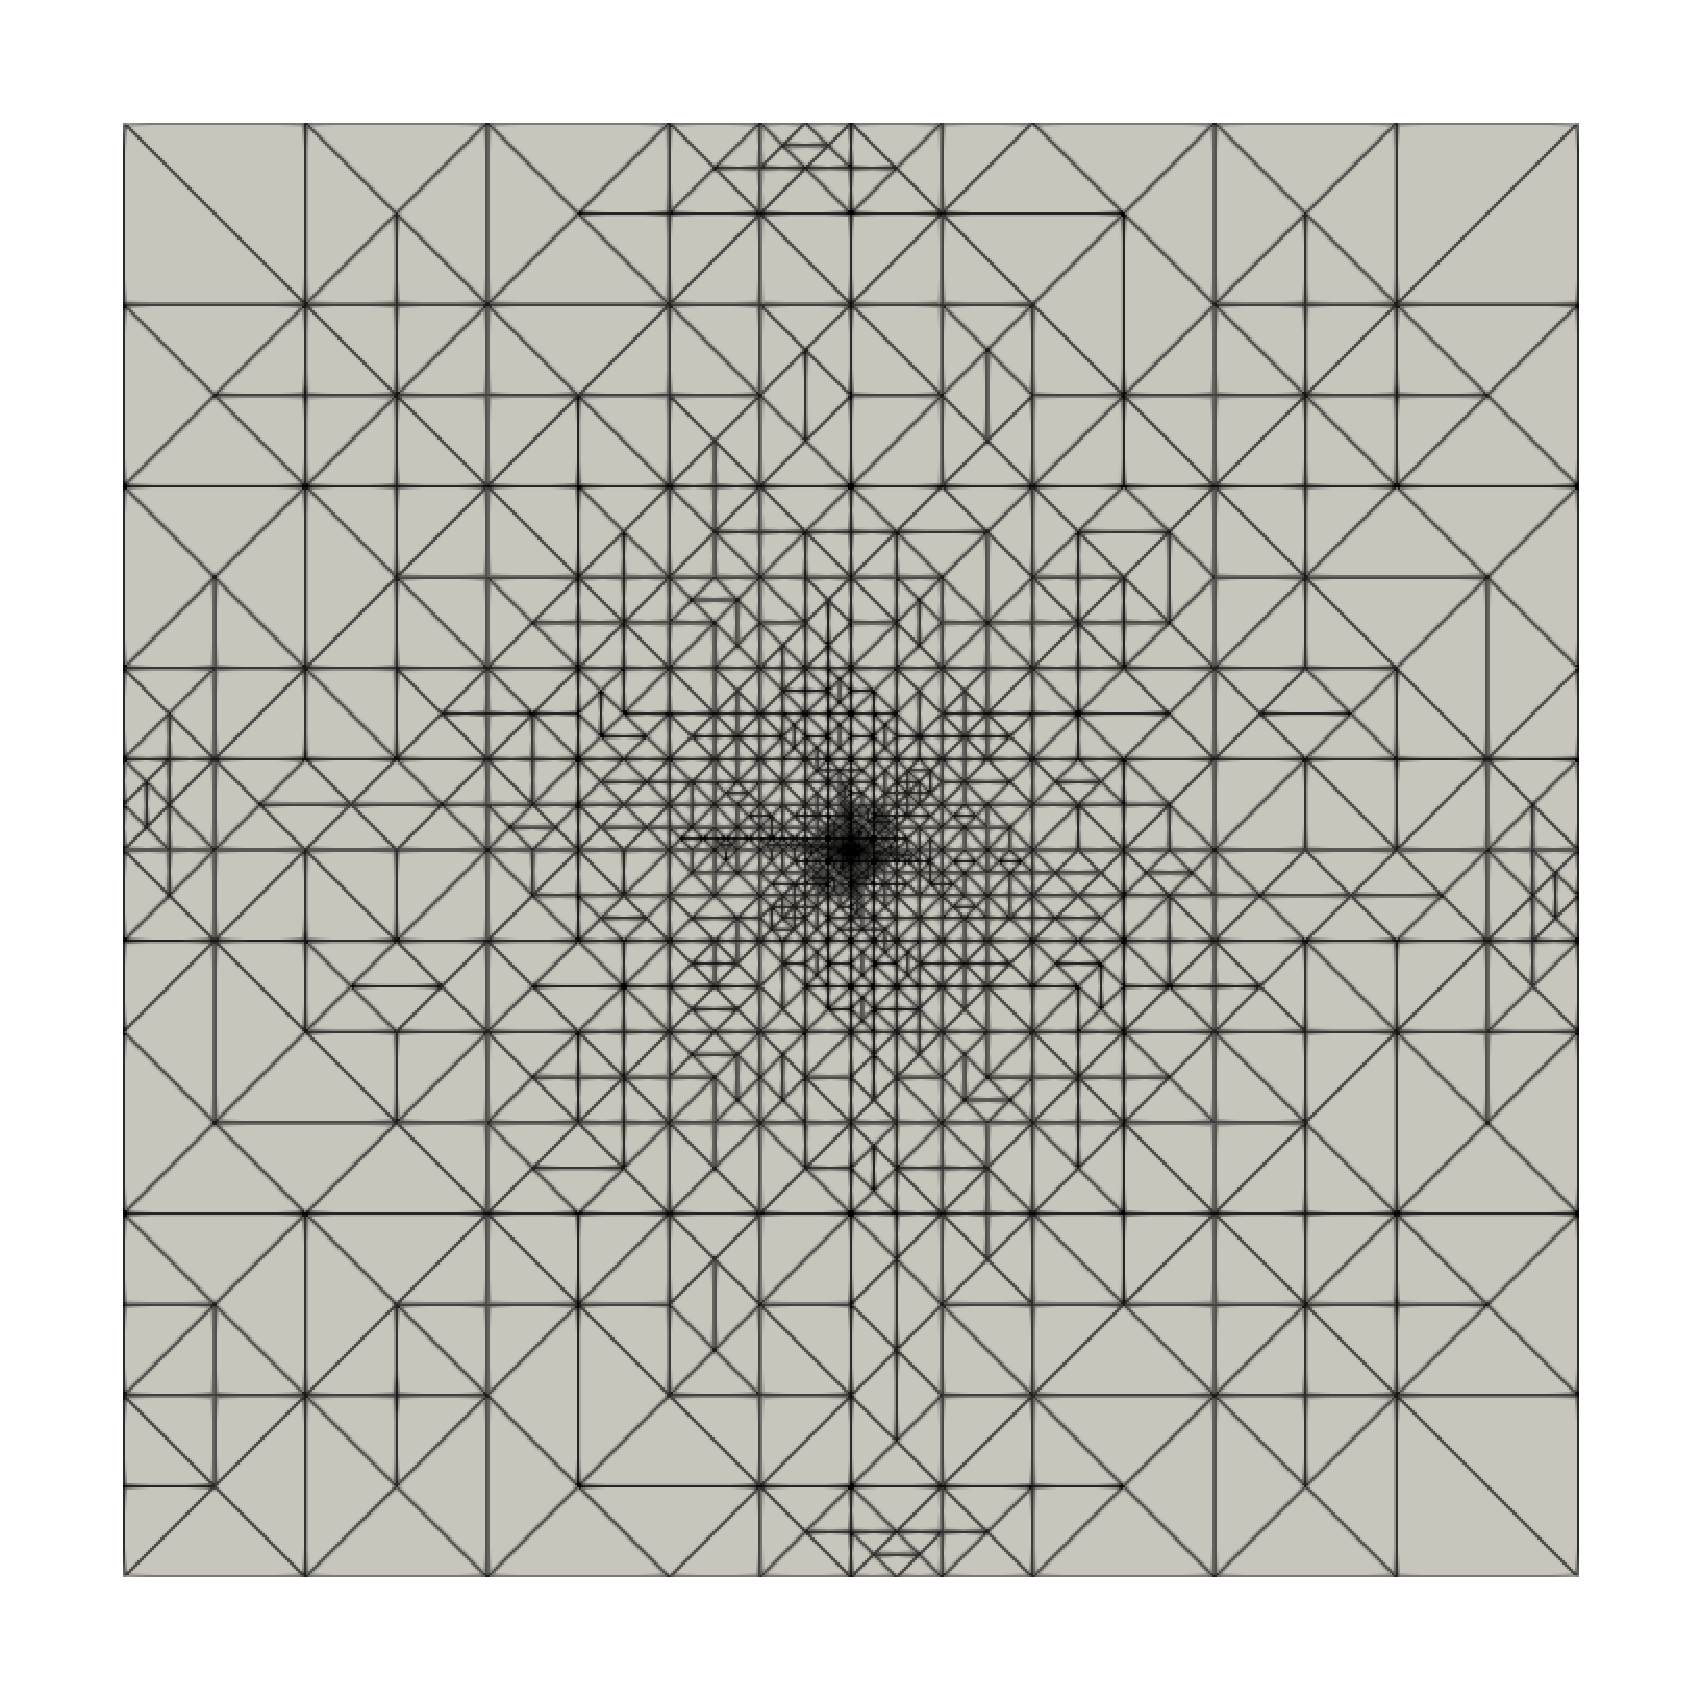
\includegraphics[width=\textwidth]{Riviere-100_P1_RT2_Mesh.pdf}
        \caption{}
        \label{fig:poisson-riviere_refmesh-p1}
    \end{subfigure}
    \hfill
    \begin{subfigure}[b]{0.32\textwidth}
        \centering
        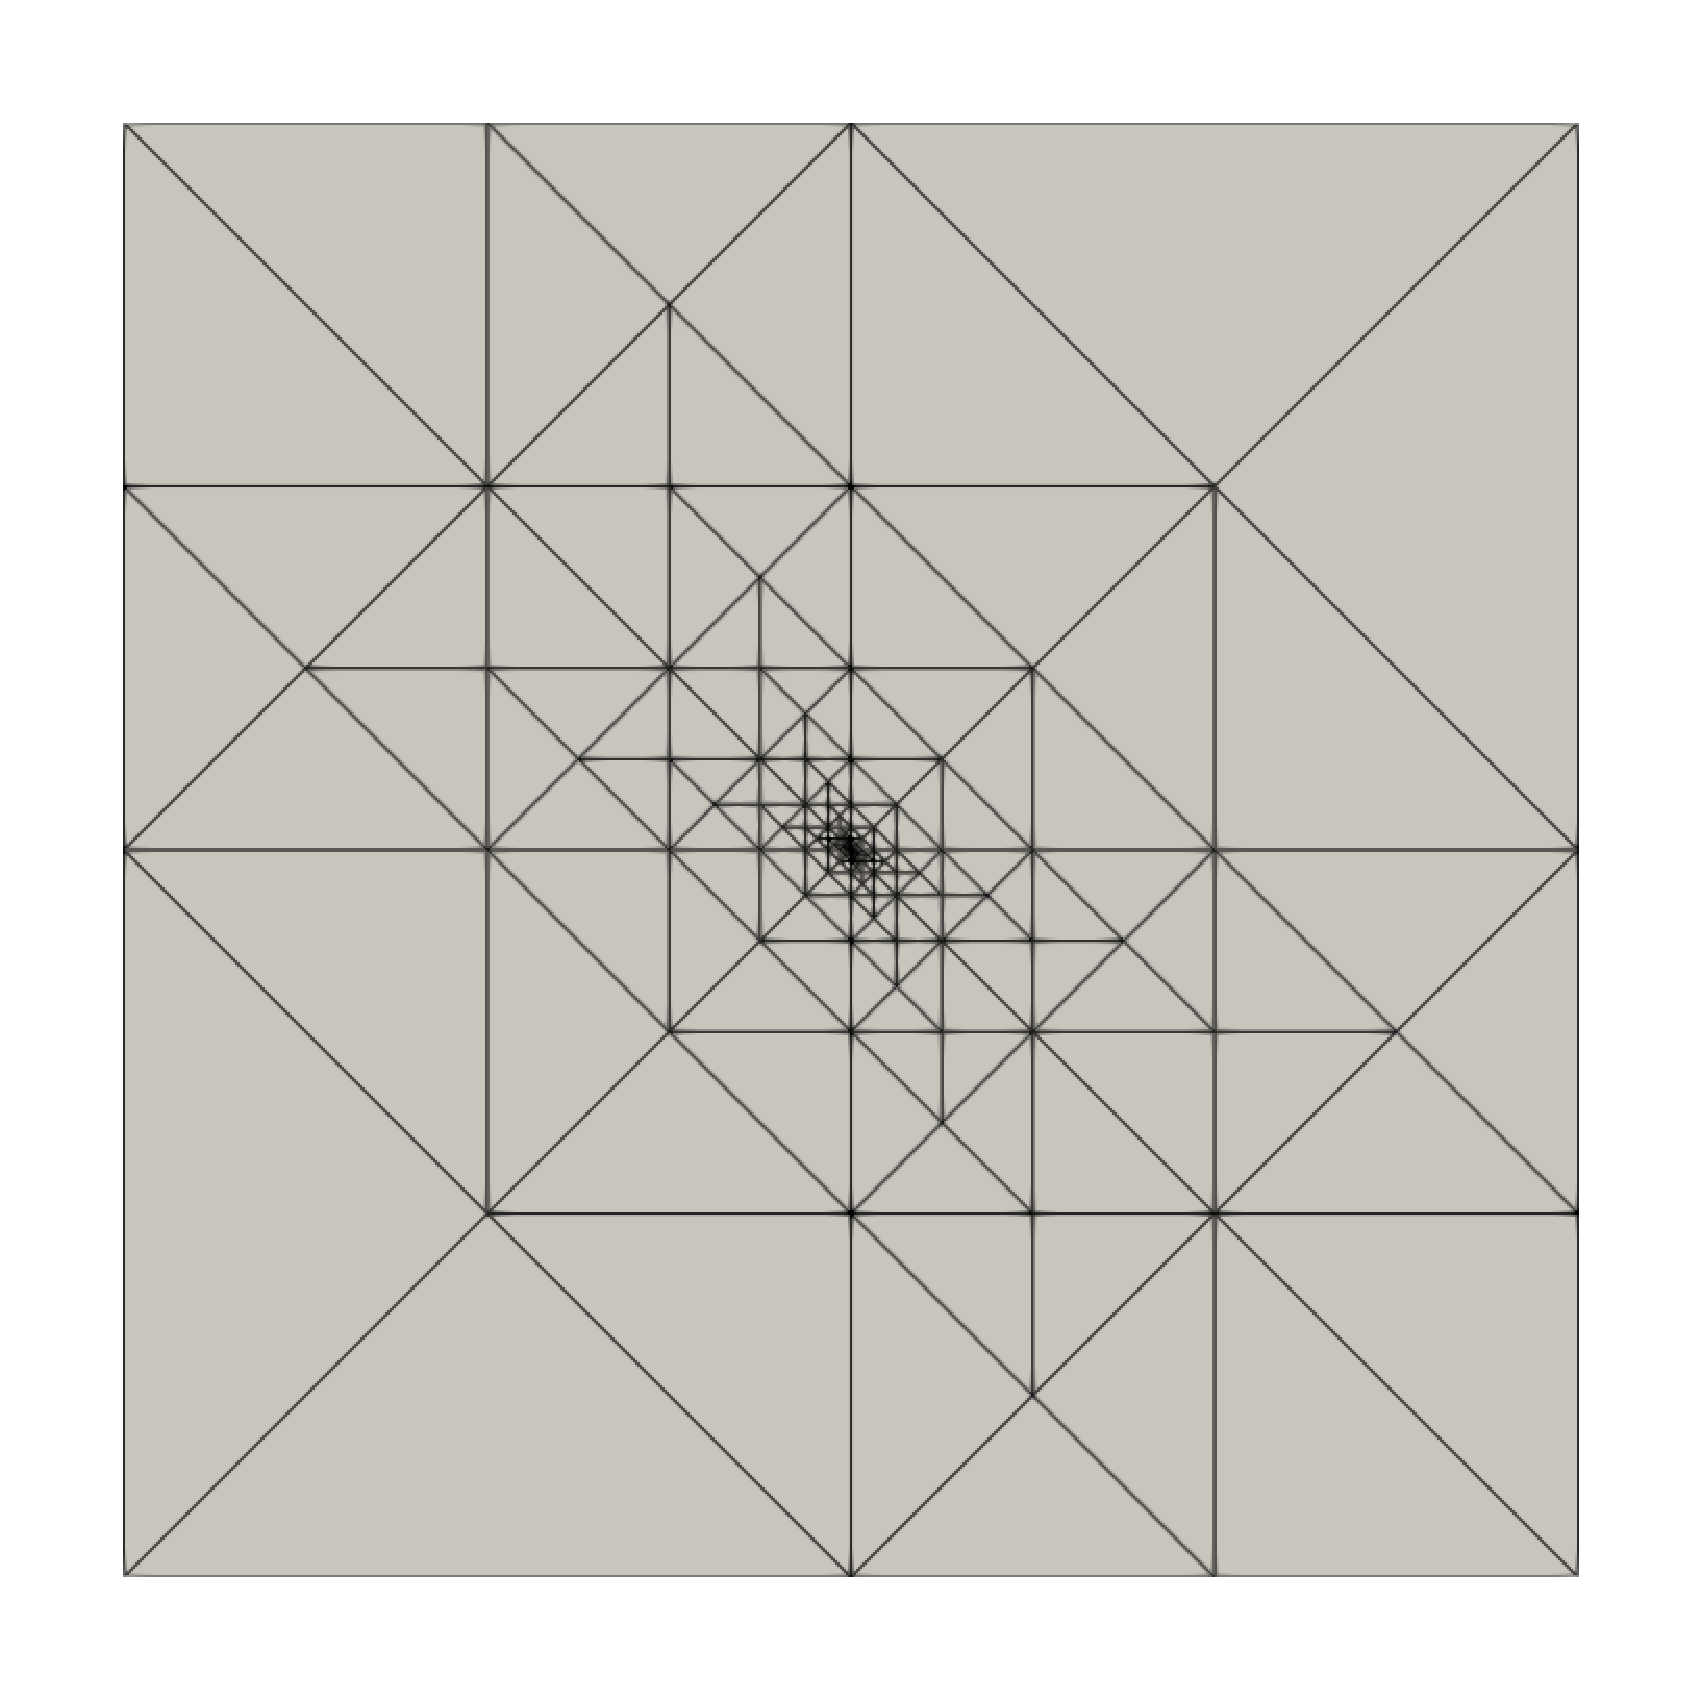
\includegraphics[width=\textwidth]{Riviere-100_P2_RT3_Mesh.pdf}
        \caption{}
        \label{fig:poisson-riviere_refmesh-p2}
    \end{subfigure}
    \caption{Results of adaptive finite element calculations with different orders $k$ and $m$. E.o.c and $\mathrm{i_{eff}}$ after the final refinement step are reported in (a).The two final meshes for $\kappa_1=100$ are depicted for $k=m-1=1$ in (b) and for $k=m-1=2$ in (c).}
    \label{fig:poisson-riviere}
\end{figure}

\begin{wrapfigure}{r}{0.4\textwidth}
\centering
\includegraphics[scale=1.0]{fig_cooks-membrane.pdf}
\caption{Cooks membrane.}
\label{fig:cook_definition}
\end{wrapfigure}
\textbf{Example 2:} Based on the Poisson equation, the influence of the equilibration order $m$ on the efficiency of the resulting estimate is shown.
Using the Cooks membrane in \Cref{fig:cook_definition}, this analysis is extended to linear elasticity, where the symmetry of the stress tensor is considered in a weak sense.
This analysis considers $\Pi_1=2.333$, $t=0.03$, and adaptive meshes based on a Dörfler marking strategy with $\theta=0.6$.
Characteristics of the first mesh satisfying $\vert\vert\vert \Displacement - \Displacement_\h \vert\vert\vert \leq 10^{-3}$ are summarised in \Cref{fig:cook_results-summary}. Since $\LinPKEqlbH$ exactly fulfils the divergence condition from \Cref{def:equilibrated_stress}, $\eta$ reduces to the sum of the $\mathcal{A}$-norm of the stress difference $\LinPKEqlbH - \stressPKLin_\h$ and the norm of asymmetric part of $\LinPKEqlbH$.
Following \Cref{fig:cook_results-summary}, the estimate is clearly dominated by the second part.
Using equilibrated stresses of order $m=k+1$ increases the efficiency, with a relative reduction (compared to the case with $m=k$) comparable to those in the Poisson example.
Increasing the accuracy of the error estimate affects the effectivity of the adaptive solution procedure -- measured by the number of degrees of
freedom required for a certain error -- in a positive way.
This trend is clearly much more pronounced for $k=2$, whereby a similar accuracy is achieved with $47\%$ fewer degrees of freedom.
A practical shortcut -- equilibration for $m=k+1$ is significantly more expensive than for $m=k$ -- appears to be the heuristic error indicator
\begin{eqnarray}
    \eta = \norm{\LinPKEqlbH - \stressPKLin_\h}\; ,
    \label{eq:elasticity_heuristic-ei}
\end{eqnarray}
where no weak symmetry is enforced on $\LinPKEqlbH$.
This yields efficiency indices close to one (see \Cref{fig:cook_results-summary}) and, comparing the convergence history in \Cref{fig:cook_results-convhist}, yields slightly better results as the guaranteed estimate with $m=k+1$.
\begin{figure}
    \centering
    \begin{subfigure}[b]{0.4\textwidth}
        \begin{tabular}{@{}l|c|c|ccc|l@{}}
            \toprule
            $k$ & $m$ & $n_\mathrm{DOF}$ & $\mathrm{err}$ & $\eta$ & $\eta _\mathrm{as}$ & $\mathrm{i_{eff}}$ \\ \midrule
            2 & 2 & 34070 & $0.0009$ & $0.009$ & $0.009$ & $10.7$ \\
            2 & 3 & 23202 & $0.0010$ & $0.008$ & $0.007$ & $7.9$ \\
            3 & 3 & 6656  & $0.0009$ & $0.020$ & $0.016$ & $17.0$ \\
            3 & 4 & 7100  & $0.0007$ & $0.009$ & $0.009$ & $13.0$ \\ \midrule
            2 & $2^*$ & 27788 & $0.0008$ & $0.001$ & $-$ & $1.5$ \\
            2 & $3^*$ & 26538 & $0.0008$ & $0.001$ & $-$ & $1.2$ \\
            3 & $3^*$ & 5738  & $0.0009$ & $0.001$ & $-$ & $1.5$ \\
            3 & $4^*$ & 5996  & $0.0008$ & $0.001$ & $-$ & $1.2$ \\ \bottomrule
        \end{tabular}
        \vspace{1.1cm}
        \caption{}
        \label{fig:cook_results-summary}
    \end{subfigure}
    \hfill
    \begin{subfigure}[b]{0.58\textwidth}
        \centering
        \includegraphics[scale=1.0]{fig_cook-convhistory.pdf}
        \caption{}
        \label{fig:cook_results-convhist}
    \end{subfigure}
    \caption{Effectivity of the different adaptive solution procedures for Cook's membrane: (a) summarises the results for the first mesh with $\mathrm{err} = \vert\vert\vert \Displacement - \Displacement_\h \vert\vert\vert \leq 10^{-3}$, (b) details the convergence history (black, $k=2$; blue, $k=3$). Orders $m^*$ indicate the use of \eqref{eq:elasticity_heuristic-ei}.}
    \label{fig:linelast-cook_results}
\end{figure}

Up to this point, only the accuracy of the error estimates has been compared. 
In the following, the focus will be on the total solution time $t_\mathrm{tot}$, which comprises $t_\mathrm{prime}$ -- the time for assembly and solution, using PETSc and MUMPS, of the primal problem -- and $t_\mathrm{eqlb}$, the time to perform the equilibration.
Comparing in a first step the relative equilibration costs $t_\mathrm{eqlb}/t_\mathrm{tot}$ for the Cook's membrane with fixed meshes in \Cref{fig:cook_performance-uniform}, one finds that -- for a primal problem of sufficient size -- $t_\mathrm{eqlb}$ is considerably smaller than $t_\mathrm{prime}$.  
Increasing $k$ increases the effort required for equilibration, while an equilibration with $m=k+1$ is significantly more expensive than the respective lowest-order case $m=k$. Similar timings for the adaptive solution of the Cook's membrane (timings are accumulated until $\vert\vert\vert \Displacement - \Displacement_\h \vert\vert\vert \leq 10^{-3}$) are summarised in \Cref{fig:cook_performance-adaptive}.
While the total solution time is dominated by the solution of the primal problem for the cases $k=m=2$, this trend is reversed for the more accurate (guaranteed) estimate with $k=m-1=2$.
Even though this case has the fewest primal degrees of freedom, the entire solution time is the longest due to the high computational costs for the equilibration.
Using primal approximations based on $k=3$ reduces the overall computation time but leads to equilibration taking up a significant share of the total computation time, an effect amplified by the small sizes of the primal problems.
As for $k=2$, the heuristic indicator \eqref{eq:elasticity_heuristic-ei} with $m=k$ performs best, and the higher-order estimate with $m=k+1$ is outperformed.
These results will clearly have to be reevaluated in a parallel context -- which is beyond this chapter's current scope -- as well as for larger primal problems.
\begin{table}[]
\centering
    \begin{subtable}[b]{0.6\textwidth}
        \centering
        \begin{tabular}{@{}c|ccc||c|ccc@{}}
        \toprule
        \multicolumn{4}{c}{$k=2$}    & \multicolumn{4}{c}{$k=3$}    \\ \midrule
        $n_\mathrm{DOF}\,\setminus\, m$ & 2    & $2^*$    & 3    & $n_\mathrm{DOF} \,\setminus\, m$ & 3    & $3^*$    & 4    \\ \midrule
        $3.49 \cdot 10^3$  & 36.3 & 27.4 & 66.4 & $3.31 \cdot 10^3$ & 45.4 & 37.9 & 63.1 \\
        $1.36 \cdot 10^4$  & 22.0 & 15.1 & 49.4 & $1.30 \cdot 10^4$ & 33.6 & 27.0 & 51.7 \\
        $2.14 \cdot 10^5$  & 15.3 & 10.2 & 38.6 & $2.04 \cdot 10^5$ & 24.5 & 19.3 & 40.9 \\
        $8.54 \cdot 10^5$  & 12.6 & 8.34 & 33.7 & $8.13 \cdot 10^5$ & 20.7 & 16.2 & 35.6 \\ \bottomrule
        \end{tabular}
        \vspace{0.2cm}
        \caption{}
        \label{fig:cook_performance-uniform}
    \end{subtable}
    \hfill
    \begin{subtable}[b]{0.38\textwidth}
        \centering
        \begin{tabular}{@{}l|c|ccc@{}}
            \toprule
            $k$ & $m$ & $t_\mathrm{prime}$ [s] & $t_\mathrm{tot}$ [s] & ratio [\%] \\ \midrule
            2 & 2     & $0.47$ & $0.61$ & 23.2\\
            2 & $2^*$ & $0.38$ & $0.45$ & 16.4\\
            2 & 3     & $0.31$ & $0.65$ & 52.7 \\ \midrule
            3 & 3     & $0.09$ & $0.15$ & 41.9\\
            3 & $3^*$ & $0.07$ & $0.11$ & 35.6\\
            3 & 4     & $0.10$ & $0.26$ & 60.5\\ \bottomrule
        \end{tabular}
        \caption{}
        \label{fig:cook_performance-adaptive}
    \end{subtable}
    \caption{Performance measurements based on Cook's membrane. (a) The $\mathrm{ratio} = t_\mathrm{eqlb} / t_\mathrm{tot}$ as a percentage for different primal problems. (b) Accumulated timings using an adaptive algorithm until $\vert\vert\vert \Displacement - \Displacement_\h \vert\vert\vert \leq 10^{-3}$. Orders $m^*$ indicate the use of \eqref{eq:elasticity_heuristic-ei}.}
    \label{fig:linelast-cook_performance}
\end{table}

\section{Conclusions}
Within this chapter, dolfinx\_eqlb, a FEniCSx-based library for the efficient equilibration of fluxes and stresses, has been introduced. 
Characteristic examples for the Poisson problem and linear elasticity highlight the library's applicability.
Additionally, an efficient but heuristic error indicator for elasticity has been introduced that neglects the asymmetry of the equilibrated stress.
In our future work, we must still prove the efficiency of the implementation and the heuristic error indicator for real-world problems. 
We further intend to generalise the implementation to 3D domains and multiphysical problems such as poroelasticity.
\vspace{-0.1cm}
\subsection*{Supplementary material}
This work is based on dolfinx\_eqlb v1.2.0 (\url{https://github.com/brodbeck-m/dolfinx_eqlb/tree/v1.2.0}). 
The examples presented can be accessed via either GitHub (\url{https://github.com/brodbeck-m/AFEM-by-Equilibration}) or, containing a Docker image, \cite{DatsetPaper}.
\vspace{-0.1cm}
\bibliographystyle{spbasic}
\bibliography{chapters/brodbeck/bibliography.bib}






% Write the full path to the location of the graphics relative to book.tex
\graphicspath{{chapters/habera/graphics/}}

% \linenumbers

\title{The FEniCS Project on AWS Graviton3}
\titlerunning{The FEniCS Project on AWS Graviton3}

\author{M.~Habera and J.~S.~Hale}
\authorrunning{Habera and Hale}

\institute{
    M.~Habera \email{michal.habera@rafinex.com} \at Rafinex SARL, and Institute of Computational Engineering, Department of Engineering, Faculty of Science, Technology and Medicine, University of Luxembourg\\
    \and
    J.~S.~Hale \email{jack.hale@uni.lu} \at Institute of Computational Engineering, Department of Engineering, Faculty of Science, Technology and Medicine, University of Luxembourg, Luxembourg}

\maketitle

\abstract{ARM architecture central processing units are increasingly prevalent
in high-performance computers due to their energy efficiency, scalability, and
cost-effectiveness. The overall goal of this study is to evaluate the
suitability of ARM-based cloud computing instances in executing finite element
computations. Specifically, we present performance results for running the FEniCS
Project finite element software on Amazon Web Services (AWS) c7g and c7gn
instances with Graviton3 processors. These processors support the ARMv8.4-A
instruction set with Scalable Vector Extension (SVE) for Single Instruction
Multiple Data operations and the Elastic Fabric Adaptor for communications
between instances. Both clang 18 and GNU Compiler Collection 13 compilers successfully generated
optimised code using SVE instructions, ensuring that users can achieve
optimised performance without extensive manual tuning. Testing a distributed
memory parallel DOLFINx Poisson solver with up to 512 Message Passing Interface
processes, we find that the performance and scalability of the AWS instances
are comparable to those of a dedicated AMD EPYC Rome cluster installed at the University
of Luxembourg. These findings demonstrate that ARM-based cloud computing
instances, exemplified by AWS Graviton3, can be competitive for distributed
memory parallel finite element analysis.}

\section{Introduction}

The FEniCS Project~\citep{alnaes2015fenics,baratta_dolfinx_2023} has been used
to write finite element solvers for problems in fields that involve solving partial differential equations, including mathematics,
biology, physics, engineering, geophysics, and mechanics.

Exploring ARM-based processors and cloud computing instances for executing
FEniCS Project-based solvers is worthwhile due to ARM's potential advantages in
cost-effectiveness, energy efficiency, and scalability with respect to
x86-64--based machines~\citep{simakov_are_2023,suarez_comprehensive_2024}.
Examples of ARM adoption in the high-performance computing (HPC) space include the Isambard project
(Isambard 3, NVIDIA Grace, \citep{isambard}), the Mont-Blanc project (Phase 3,
Cavium Thunder X2, \citep{Rajovic2016}), the Fugaku supercomputer (Fujitsu A64FX,
\citep{fugaku}), and the Astra supercomputer (Cavium ThunderX2, \citep{astra}). Publicly available cloud services with ARM instances include those of Amazon Web
Services AWS (Graviton3 CPU based on Neoverse V1 and Graviton4 CPU with
Neoverse V2), Google Cloud (Axion CPU based on Neoverse V2,
\citep{google_arm_compute}), and Microsoft Azure (Azure Cobalt 100 based on
Neoverse N2, \citep{microsoft_azure}).

AWS Graviton3-based instances aim to provide cost-effective computing resources
for scientific computing and machine learning applications by including both
Scalable Vector Extension (SVE) instructions for Single Instruction Multiple
Data (SIMD) parallelism and the Elastic Fabric Adaptor (EFA) interconnect for
high-bandwidth low-latency communication between instances. This makes the AWS
cloud offering particularly appealing for executing scientific computing code
such as the FEniCS Project.

A key technology in the FEniCS Project is the use of automatic code generation
(compilation). The user expresses a finite element problem in Unified
Form Language (UFL)~\citep{alnaes_unified_2014}, and the FEniCSx Form
Compiler (FFCx)~\citep{kirby_compiler_2006} then compiles the UFL description of the
problem into a low-level C kernel for computing the cell-local finite element
tensor.

One aspect of good performance of a compute-bound kernel is ensuring the
assembly code of the compiled kernel contains calls to Single Instruction
Multiple Data (SIMD) operations. SIMD operations can apply the same operation
to multiple data items in a single CPU clock cycle. For a recent overview of
SIMD programming strategies, see, for example, \cite{rocke_evaluation_2023}. The current
strategy of FFCx with respect to SIMD is to ensure that its kernels are
amenable to the compiler applying automatic vectorisation, a process that
automatically converts a scalar program into a vectorised equivalent that uses
SIMD operations.
 
Consequently, to achieve good performance when using FEniCSx on
Graviton3, it is important that users verify that the latest compilers automatically
produce SVE and/or Neon SIMD instructions when compiling the generated C finite
element kernels and that these kernels display reasonable runtime performance. 

In addition to SIMD parallelisation at the kernel level, DOLFINx, the FEniCS Project's finite
element problem solving environment, also supports
distributed memory parallel assembly of global finite element data structures
(sparse matrices and vectors) using the Message Passing Interface (MPI; for
full details, see \cite{baratta_dolfinx_2023}). Users running large-scale
DOLFINx simulations on AWS must verify that the EFA interconnect's performance is sufficient for parallel scalability.

In summary, the contribution of this chapter is to examine both the SIMD
performance and multi-node parallel scaling of the FEniCS Project's software on
Amazon's Graviton3-based instances. 

\section{Methodology and Results}

\subsection{Systems}
AWS c7g and c7gn instances are compared to the Aion computing instances available
at the University of Luxembourg's HPC facilities \citep{VCPKVO_HPCCT22}. These
instances have different hardware configurations (see
\cref{tab:aion-aws-config} for full details).

The FEniCS Project components are written in a mixture of Python, 'modern' C++20 and Standard C17. The Python interface is a wrapper around the core data
structures and computationally intensive algorithms written in C and C++.

\begin{table}
    \resizebox{\columnwidth}{!}{%
  \footnotesize
  \renewcommand{\arraystretch}{1.5}
  \begin{tabular}{l|l|l}
                              & Aion node                                                          & AWS c7g instance \\ \hline \hline
    Processor                 & \makecell[l]{2 x (AMD EPYC ROME 7H12, \\ 64 cores @ 2.6 GHz)}      & \makecell[l]{1 x (Graviton3, \\ 64 cores @ 2.6 GHz)} \\ \hline
    Architecture              & x86\_64, Zen 2 (AVX2)                                              & ARMv8.4-A, Neoverse V1 (SVE) \\ \hline
    Memory                    & \makecell[l]{256 GB DDR4 \\ 3200 MT/s = 25.6 GB/s \\ 8 non-uniform memory access (NUMA) nodes} & \makecell[l]{128 GB DDR5 \\ 4800 MT/s = 38.4 GB/s  \\ Uniform memory access (no NUMA) } \\ \hline
    Total mem. bandwidth      & 2 x 200 GB/s                                                       & 1 x 300 GB/s  \\ \hline
  \end{tabular}
    }
  \vspace{5pt}
  \caption{Configuration of the Aion nodes (University of Luxembourg's HPC facilities) and
	AWS c7g (Amazon) instances. The c7gn instance used in the Poisson weak
	scaling test has the same hardware as c7g with the addition of a
	$\SI{200}{\giga\byte\per\second}$ interconnect between instances for
	MPI-based communication.}
  \label{tab:aion-aws-config}
\end{table}

\subsection{Memory Bandwidth}
Low-order finite element methods are typically memory bandwidth constrained, since 
the time to load and store data from main memory (e.g. the mesh geometry)
dominates the time to perform the arithmetic operations to compute the
finite element cell tensor. Understanding a processor's memory bandwidth is therefore important for ensuring optimal performance.

STREAM \citep{McCalpin1995,McCalpin2007} is the industry standard benchmark for
measuring sustained memory bandwidth performance, with McCalpin estimating memory bandwidth
from memory-intense operations (copy, scale, add) on large contiguous arrays.

\Cref{fig:stream-single} shows the results for the copy operation for a single-node
benchmark. For the single-node benchmark, $80 \%$ of the
theoretical peak memory bandwidth of $\SI{400}{\giga\byte\per\second}$ for Aion
and $\SI{300}{\giga\byte\per\second}$ for AWS c7g is reached. This is considered
a reasonable outcome of the STREAM benchmark \citep{McCalpin2023}. Bandwidth
saturation is observed at around $20 \%$ of the node utilization.
Both curves show different saturation point characteristics due to
different memory access configurations. On the Aion instances, there are eight NUMA nodes of 16 cores each, while AWS c7g instances are set up with unified memory access.
\vspace{-5mm}
\begin{figure}
\begin{center}
        \includegraphics{chapters/habera/graphics/stream_plots/stream_single_node.pdf}
\end{center}
	\caption{Single-node STREAM benchmark. The theoretical peak bandwidth of each system is shown as a dashed line.}
        \label{fig:stream-single}
\end{figure}

\subsection{Finite Element Kernels}
To measure the performance of standard FEniCS user finite element
code, we use the Local Finite Element Operator Benchmarks repository
\citep{Baratta2023}. The benchmark measures the execution time of a local finite
element kernel generated by the FFCx v0.9.0
\citep{kirby_compiler_2006}. We generate a matrix-free three-dimensional
Laplace kernel representing finite element discretization of the action of
Laplace operator $A_{ij}$ with spatially varying material property $\kappa(x)$:
\begin{align}
    v_i = A_{ij} w_j, \quad
    A_{ij} = \int_K \kappa J_{mk} J_{mn} \nabla_k \phi_i \nabla_n \phi_j |\det J| \mathrm dx,
\end{align}
where $K$ is a fixed reference tetrahedron; $w_j \in \mathbb{R}^{n}$ is a
fixed, prescribed vector; $J$ is a Jacobian transformation matrix; and the $\phi$ terms 
are finite element basis functions.

The generated kernel calculates a double-precision vector $v_i \in
\mathbb{R}^{n}$, where $n = 4$ for first-order (low-order) discretization and
$n = 165$ for eighth-order (high-order) discretization. Low-order kernels are
expected to be memory bandwidth limited, while high-order kernels have higher
arithmetic intensity. In addition, the matrix-free (operator action) version
requires fewer load and store operations in comparison to the assembly of a
matrix, increasing the ratio of floating-point operations to memory loads and
stores. Consequently, significant performance improvements are possible for high-order kernels if the compiler can automatically emit SIMD
operations.

\paragraph{Generated Code Structure.}

Compiler (loop) SIMD auto-vectorisation is usually performed for innermost
loops with known compile time bounds. Analysis of the FFCx autogenerated code
is required to understand the potential and determine missed optimisations.

\begin{lstlisting}[language=c,
    caption=Abbreviated FFCx-generated finite element kernel,
    style=CStyle,
    label=lst:c-code]
void kernel(double* restrict A, const double* restrict w, ...){
    // 1. Static arrays of basis functions and quadrature weights.
    // 2. Quadrature rule--independent computations.

    for (int iq = 0; iq < NUM_QUAD_POINTS; ++iq) {
        // 3. Quadrature loop body.
        for (int ic = 0; ic < NUM_DOFS; ++ic){
            // 3.1 Coefficient evaluation.
            w1_d100 += w[4 + (ic)] * FE0_C0_D100_Q530[0][0][iq][ic];
            // ...
        }

        // 3.2 Scalar graph evaluation.
        double sv_530_0 = w1_d100 * sp_530_18;
        double sv_530_1 = w1_d010 * sp_530_22;
        // ...

        for (int i = 0; i < NUM_DOFS; ++i) {
            // 3.3 Tensor assignment loop.
            A[(i)] += fw0 * FE0_C0_D100_Q530[0][0][iq][i];
            // ...
        }
    }
}
\end{lstlisting}

An abbreviated example of generated C code is shown in
\cref{lst:c-code}. First, there are arrays defining finite element basis
functions at quadrature points. These require no arithmetic operations.
Computations independent of the quadrature loop contain more intense arithmetic
operations (e.g. determinant of the Jacobian) but are executed only once.
Non-affine geometry would require the evaluation of geometric quantities at each
quadrature point, which would increase the arithmetic intensity and yield more
opportunities for vectorisation.

The most performance-critical part of the code is contained in the quadrature
loop body. For the eighth-order Laplace operator, \lstinline{NUM_QUAD_POINTS = 214} and \lstinline{NUM_DOFS = 165}. There are two
innermost loops: coefficient evaluation and tensor assignment. Both contain a
set of multiply--add operations that are candidates for automatic vectorisation
via fused multiply--add operations in both the SVE (Graviton3) and AVX2 (AMD EPYC) cases.

\paragraph{Experimental Results.}

For the finite element kernel benchmarks, we compile the kernels with
LLVM/clang 18.1.3 and GNU Compiler Collection (GCC) 13.2.0. Full details are provided in
\cref{tab:compilers-kernels}.

\begin{table}
    \centering
    \footnotesize
    \renewcommand{\arraystretch}{1.5}
    \begin{tabular}{l|l|l|l}
                                    & Compiler     & Aion                                                                                            & AWS c7g \\ \hline \hline
        Ofast, native, vectorised   & GCC 13.2.0   & \makecell[l]{-Ofast \\ -march=znver2 \\ -mtune=znver2}                                          & \makecell[l]{-Ofast \\ -mcpu=neoverse-v1} \\ \hline
                                    & clang 18.1.3 & \makecell[l]{-Ofast \\ -march=znver2 \\ -mtune=znver2}                                          & \makecell[l]{-Ofast \\ -mcpu=neoverse-v1} \\ \hline
        Ofast, native, no vec.      & GCC 13.2.0   & \makecell[l]{-Ofast \\ -march=znver2 \\ -mtune=znver2 \\ -fno-tree-vectorize}                   & \makecell[l]{-Ofast \\ -mcpu=neoverse-v1 \\ -fno-tree-vectorize} \\ \hline
                                    & clang 18.1.3 & \makecell[l]{-Ofast \\ -march=znver2 \\ -mtune=znver2 \\ -fno-slp-vectorize \\ -fno-vectorize}  & \makecell[l]{-Ofast \\ -mcpu=neoverse-v1 \\ -fno-slp-vectorize \\ -fno-vectorize} \\ \hline
        O2, no vec.                 & GCC 13.2.0   & \makecell[l]{-O2 \\ -fno-tree-vectorize}                                                        & \makecell[l]{-O2 \\ -fno-tree-vectorize} \\ \hline
                                    & clang 18.1.3 & \makecell[l]{-O2 \\ -fno-slp-vectorize \\ -fno-vectorize}                                       & \makecell[l]{-O2 \\ -fno-slp-vectorize \\ -fno-vectorize} \\ \hline
    \end{tabular}
    \vspace{5pt}
    \caption{Compiler versions and compilation flags used for finite element kernel benchmarks}
    \label{tab:compilers-kernels}
\end{table}

The kernel benchmark results are presented in \cref{fig:local-deg1,fig:local-deg8}. Low-order kernels (\cref{fig:local-deg1}) show no
dependence on the compiler vectorisation setup. On the other hand, AWS c7g demonstrates a
$1.3\times$ speedup over Aion, which we attribute to greater memory bandwidth for  a
single process.

High-order kernels (\cref{fig:local-deg8}), which are expected to benefit from
SIMD operations, reveal a clear link between compiler settings and performance.
Both clang and GCC auto-vectorisers perform well, producing a noticeable
speedup (\textgreater $2\times$) in the most optimised setting. The vectorisation
speedup (\textgreater $4\times$) is more significant with the Aion nodes.

\begin{figure}
    \begin{subfigure}{.5\textwidth}
        \centering
        \includegraphics{chapters/habera/graphics/kernel_plots/local_operator_clang_deg1.pdf}
        \caption{clang 18.1.3}
        \label{fig:local-clang-deg1}
    \end{subfigure}%
    \begin{subfigure}{.5\textwidth}
        \centering
        \includegraphics{chapters/habera/graphics/kernel_plots/local_operator_gcc_deg1.pdf}
        \caption{GCC 13.2.0}
        \label{fig:local-gcc-deg1}
    \end{subfigure}
    \caption{Low-order Laplace operator action assembly}
    \label{fig:local-deg1}
\end{figure}

\begin{figure}
    \begin{subfigure}{.5\textwidth}
        \centering
        \includegraphics{chapters/habera/graphics/kernel_plots/local_operator_clang_deg8.pdf}
        \caption{clang 18.1.3}
        \label{fig:local-clang-deg8}
    \end{subfigure}%
    \begin{subfigure}{.5\textwidth}
        \centering
        \includegraphics{chapters/habera/graphics/kernel_plots/local_operator_gcc_deg8.pdf}
        \caption{GCC 13.2.0}
        \label{fig:local-gcc-deg8}
    \end{subfigure}
    \caption{High-order Laplace operator action assembly}
    \label{fig:local-deg8}
\end{figure}

Optimisation reports (\texttt{-Rpass=loop-vectorize} for clang,
\texttt{-fopt-info-vec-optimised} for GCC) and analysis of the generated
assembly reveal that, for low-order operator action, using the \lstinline{-Ofast} compiler optimisation
level enhances constant folding and allows more operations to be computed at compile time (e.g. partial sums of the static constant arrays)
\citep{GodboltArmClangDeg1}.

On Graviton3, both GCC and clang generate SVE floating-point
fused multiply--add (FMLA) instructions
\citep{ArmReferenceManual} for both the coefficient evaluation and tensor
assignment loops \citep{GodboltArmClang,GodboltArmGCC}. FMLA is a SIMD instruction that multiplies two vectors stored in
SVE registers and adds the result to a third vector. The coefficient evaluation
loop with no interdependencies between iterations is a perfect example of
compiler auto-vectorisation. Moreover, for higher-order
discretization, there is potential for exploiting wider SVE registers (up to 2,048 bits).

An assembly excerpt for the coefficient evaluation is shown below.
\begin{lstlisting}[language=c, style=CStyle]
ld1d    {z0.d}, p0/z, [x7, x0, lsl #3]
ld1d    {z25.d}, p0/z, [x3, x0, lsl #3]
fmla    z3.d, p0/m, z25.d, z0.d
...
faddv   d1, p1, z1.d
\end{lstlisting}
As expected, there are two contiguous loads LD1D in two of the available SVE
Z0--Z31 registers followed by a fused multiply--add instruction. The result is
accumulated in an SVE register Z3 that is then horizontally summed outside
of the vectorised loop (FADDV). Here P0 is a predicate register without any
constraints on the available elements.

On Aion, both GCC and clang vectorise both the coefficient evaluation and tensor
assignment loops and rely on the \lstinline{VFMADD231PD} instructions on the
YMM registers, that is, the vectorisation width of four doubles
\citep{Godboltx86Clang,Godboltx86GCC}.

\subsection{Parallel Scalability}

The parallel scalability results were obtained using performance test codes
for FEniCSx \citep{Wells2023} built against DOLFINx 0.6.0 and PETSc 3.18
\citep{petsc} with the Spack package manager setup, using GCC 12.2.0. We set up
Spack to use a version of OpenMPI provided by AWS that includes the appropriate
libfabric with native support for the EFA interconnect. Libfabric is a network
communication library that abstracts networking technologies from fabric and
hardware implementation, ensuring optimal data transfer across Amazon's
proprietary EFA interconnect.

The Poisson equation solver benchmark consists of the following measured steps:
\begin{enumerate}
    \item Create a mesh. Create a unit cube mesh and discretize using linear
    tetrahedral cells. Partition the mesh with the ParMETIS 4.0.3 partitioner
    \citep{Karypis1998} and distribute.
    \item Assemble the matrix. Execute the local Poisson equation kernel over the
    mesh and assemble into a PETSc MATMPIAIJ (distributed compressed sparse row)
    matrix.
    \item Solve the linear system. Run the Conjugate Gradient solver with a classical algebraic
    multigrid (BoomerAMG; see \citep{hypre}) preconditioner.
\end{enumerate}
Creating the mesh (including partitioning), assembling matrices, and solving the
resulting linear system are typically the most expensive steps in a finite
element solution. They also contain significant parallel communication steps that
can highlight issues in either the finite element solver or the underlying MPI
hardware/software stack, leading to poor parallel scaling. 
%
Weak scaling results (with a constant workload of approximately \SI{5e+5} degrees of freedom
per process) are shown in \cref{fig:weak-scaling}. Both Aion and AWS c7gn
show almost constant times for mesh creation ($< 5\%$ difference).

Matrix assembly is expected to have ideal weak parallel scalability due to the
cell-local nature of the assembly loop and negligible MPI
communication during matrix finalization. Aion and AWS c7gn show a small increase
in time (10--15\%) for 512 processes.

The time for the solving step increases by 40\% for 512 processes on AWS c7gn and
by 27\% on Aion. However, the number of Krylov iterations of the preconditioned
Conjugate Gradient solver grows from 16 to 20 for 512 processes (a 25\% increase) due to the
inefficiency of the algebraic multigrid preconditioner on an unstructured 3D
mesh. Taking this into account, the time per iteration is almost constant on
Aion ($< 5\%$), and a small increase of 15\% on AWS c7gn is observed.

\begin{figure}
    \begin{subfigure}{.7\textwidth}
	\begin{center}
        \includegraphics{chapters/habera/graphics/parallel_scaling_plots/output/weak_scaling_aion_poisson.pdf}
        \caption{Aion, \SI{5e+5} degrees of freedom per process, 25\% utilization (32 processes per node)}
        \label{fig:weak-scaling-aion}
	\end{center}
    \end{subfigure}

    \begin{subfigure}{.7\textwidth}
	\begin{center}
        \includegraphics{chapters/habera/graphics/parallel_scaling_plots/output/weak_scaling_aws_c7gn_poisson.pdf}
        \caption{AWS c7gn, \SI{5e+5} degrees of freedom per process, 50\% utilization (32 processes per node)}
        \label{fig:weak-scaling-aws}
	\end{center}
    \end{subfigure}
    \caption{Weak parallel scalability of the DOLFINx Poisson equation solver on Aion and AWS c7gn systems}
    \label{fig:weak-scaling}
\end{figure}

\section{Conclusions}

Benchmarks for the memory bandwidth, local finite element kernels, and parallel
scalability of a Poisson solver were executed on Aion nodes and on AWS c7g(n)
instances.

Memory bandwidth measured using STREAM MPI confirms the higher memory transfer rate
of AWS c7g(n) but the superior total bandwidth of
~\SI{310}{\giga\byte\per\second} per Aion node.

In terms of the auto-vectorisation capabilities of GCC 13.2.0 and clang 18.1.3, both
produce optimised instructions for the targeted microarchitectures (Zen 2 for
Aion and Neoverse V1 for AWS c7g). This observation is confirmed with
performance benchmarks based on local finite element kernels for the Laplace
operator.

The MPI-based distributed memory Poisson equation solver shows weak scaling with
a 15\% increase in time per iteration for 512 processes on the c7gn-based cluster.
The results for the University of Luxembourg's Aion system are slightly
superior, with almost constant ($< 5\%$ difference) times per iteration for 512
processes.

Based on our results, we conclude that AWS Graviton3 instances are a viable
alternative for HPC tasks using the FEniCS Project's
automated finite element solver. These instances are likely to be particularly
interesting for users with infrequent or highly elastic large-scale
computational demands~\citep{emeras_amazon_2016}.

In the future, we plan to work on other, more complex problems (e.g. linear
elasticity) and performance benchmarks of direct solvers. Additionally, the
latest generation Graviton4 instances provide an improved Neoverse V2
instruction set, with a smaller SVE vector length of 128 bits,
\citep{ArmReferenceManualNeoverseV2}, warranting further investigation.

\section*{Supplementary Material}
Raw data and plotting scripts are archived at \cite{habera_2024_13748405}.

\begin{acknowledgement}
This project received computing resources from Amazon Web Services (AWS)
through the first and second collaborative University of Luxembourg and
AWS Graviton3 calls. The experiments presented in this paper were
carried out using the HPC facilities of the University of Luxembourg
~\citep{VCPKVO_HPCCT22}; see \url{https://hpc.uni.lu}.

This research was funded in whole or in part, by the National Research
Fund (FNR), grant reference COAT/17205623. For the purpose of open
access, and in fulfilment of the obligations arising from the grant
agreement, the author has applied a Creative Commons Attribution 4.0
International (CC BY 4.0) license to any Author Accepted Manuscript
version arising from this submission.

JSH declares that a family member was working at Rafinex during the period
of this project. This person was not involved in this study.
\end{acknowledgement}

\bibliographystyle{spbasic}
\bibliography{chapters/habera/bibliography.bib}
 
\graphicspath{{chapters/chp1/graphics/}}
\title{cuDOLFINx: A CUDA Extension for FEniCSx}
\titlerunning{cuDOLFINx: A CUDA Extension for FEniCSx}

\author{Benjamin~A.~Pachev, James~D.~Trotter, and Igor~A.~Baratta}
\authorrunning{Pachev et al.}
\institute{Benjamin.~A.~Pachev \email{benjmainpachev@utexas.edu} \at The University of Texas at Austin, Austin, Texas, United States \\James.~D.~Trotter \email{james@simula.no} \at Simula Research Laboratory, Oslo, Norway
\\Igor~A.~Baratta \email{ia397@cam.ac.uk} \at Department of Engineering, University of Cambridge, Cambridge, United Kingdom
}


\maketitle

\abstract{This chapter introduces cuDOLFINx, a Python package that extends FEniCSx with GPU-accelerated assembly capabilities.
The extension enables FEniCSx codes to be accelerated on the GPU with minimal changes and provides an easy way for researchers to experiment with GPU-accelerated partial differential equation solvers. By contrast with previous efforts to enhance FEniCSx with GPU capabilities, cuDOLFINx is designed as a standalone package and does not require major changes to the core components of FEniCSx. Consequently, it has the potential to become a usable part of the FEniCSx ecosystem and a long-term solution to the problem of providing GPU acceleration capabilities in FEniCSx.
We further present performance benchmarks for representative GPU-accelerated FEniCSx applications on an NVIDIA GH200 GPU.
Our results indicate that GPU-accelerated assembly routines within cuDOLFINx can be up to 40 times faster than traditional FEniCSx assembly with MPI parallelization on a multi-core CPU node.}

\section{Introduction}
Graphics processing units (GPUs) provide an alternative means of parallelizing computations compared to traditional clusters of multi-core CPUs. For many applications, GPUs are more energy efficient and have thus revolutionized fields such as machine learning~\citep{navarro2014survey}. Several well-known software packages used for solving partial differential equations (PDEs) have taken steps to provide GPU acceleration capabilities, including PETSc~\citep{MILLS2021102831}, MFEM~\citep{anderson2021mfem}, libCEED~\citep{abdelfattah2021gpu}, and deal.II~\citep{arndt2021deal}.
However, the GPU acceleration of PDE solvers has yet to become the norm, since other PDE libraries~\citep{baratta2023dolfinx,schoberl2014c++,hecht2012new,moxey2020nektar++,FiredrakeUserManual} lack support for GPU acceleration. Furthermore, even when GPU acceleration is available, it often has limited support and can be difficult to use. Modifying existing code to use GPU parallelism remains a significant challenge~\citep{MILLS2021102831}. GPU programming requires a specialized compiler, memory space, and syntax, such that code must often be largely rewritten to take advantage of GPU acceleration.


A major attraction of FEniCSx~\citep{baratta2023dolfinx} as a tool for solving PDEs with the finite element method is its simple Python interface and automated generation of efficient C code. These features enable the rapid prototyping and development of performant solvers for complicated PDEs. Our goal in developing cuDOLFINx \citep{cudolfinxzenodo} is to enable FEniCSx users to add GPU acceleration to their existing PDE solvers with minimal effort.
GPUs are attractive for PDEs due to their increased throughput, high number of floating-point operations per second (FLOPS), and memory bandwidth. Although many PDEs are generally memory bound, even memory-bound problems can benefit significantly from GPU acceleration. The remainder of this chapter will provide a brief overview of cuDOLFINx; present example applications for the Poisson, Navier--Stokes, and shallow water problems; and, finally, discuss the future development of cuDOLFINx.

\section{Overview of cuDOLFINx}
The two most expensive steps in the finite element method are linear solves and the assembly of matrices or vectors.
We would like to accelerate both of these steps with GPUs, partly to minimize expensive copies to and from GPU memory.
The PETSc~\citep{MILLS2021102831}, Ginkgo~\citep{ginkgo-toms-2022}, AMGx~\citep{naumov2015amgx}, hypre~\citep{li2020efficient,falgout2021porting}, SuperLU~\citep{li2023newly}, and other libraries~\citep{lu2023tilesptrsv} provide efficient GPU-accelerated linear solvers.
The goal of cuDOLFINx is to enable GPU-accelerated assembly so that the entirety of FEniCSx finite element workflows can be GPU accelerated.

FEniCSx relies on auto-generated kernels to perform element-wise numerical integration, and the resulting element matrices or vectors can be assembled to form global matrices or vectors.
In cuDOLFINx, these kernels are modified to execute on a GPU using CUDA.
The generated kernels from the FEniCSx Form Compiler (FFCx) are used as is, with no GPU-targeted changes.
Each element is processed by a single GPU thread, and atomic operations are used to prevent data races.
This approach works well for low-order elements but can be problematic for higher orders, since the computation of element stiffness matrices at high orders can require more local memory than is available to a single GPU thread. This can increase the usage of slower memory and reduce the number of GPU threads that can execute concurrently. Consequently, GPU assembly routines for high-order methods typically assign multiple threads to each element~\citep{MACIOL20101093,dziekonski2013generation,abdelfattah2021gpu,swirydowicz2019acceleration}.
This is a goal of future work and will require extending FFCx to support GPU parallelism within element kernels.

In addition to the element-wise kernels, cuDOLFINx provides GPU-based assembly loops to assemble the local contributions from each element into global matrices or vectors. This requires information about the mesh, boundary conditions, and function spaces to be copied to GPU memory. Internally, cuDOLFINx provides GPU counterparts for many of the data structures used in FEniCSx and automatically performs the data transfer to the GPU. Once the data are transferred, they are expected to remain on the GPU, though mechanisms exist for moving data between the CPU and GPU when necessary.

The cuDOLFINx package extends the work of \cite{trotter2023targeting}. In addition to major modifications needed to support DOLFINx 0.9 (the most recent version at the time of writing), the following new features have been developed:
\begin{enumerate}
    \item Support for boundary integrals was developed from scratch and considerably improved compared to the original version of the code, which only supported boundary integrals in very limited scenarios.
    \item To support discontinuous Galerkin (DG) methods, integrals on interior mesh edges are required. This functionality was added to the original GPU-accelerated code.
    \item Most FEniCSx users utilize the Python version of the library. Consequently, a Python API was developed for the GPU acceleration capabilities. It was designed to be much simpler to use than the original C++ interface, without loss of functionality.
    \item The GPU acceleration scheme was applied to a wider range of problems, including the Navier--Stokes and shallow water equations.
\end{enumerate}

There are three main cuDOLFINX software components.
The first is a set of C++ classes containing the CUDA data structures needed for assembly.
These classes correspond to their DOLFINx counterparts and are responsible for copying the required data to the GPU.
The second consists of C++ classes that manage the generation, runtime compilation, and launching of CUDA assembly kernels.
The final component contains the Python bindings for the C++ core. Most users will only need to utilize the Python wrapper, which provides Python versions of the C++ CUDA data structure classes, as well as convenience routines for performing assembly operations.
We demonstrate the Python wrapper's usage in the following section.
\section{Sample Usage}

Using cuDOLFINx within existing FEniCSx code requires only minor modifications. Consider the following example for solving Poisson's equation on the unit square:
\begin{python}
from mpi4py import MPI
from dolfinx import fem, mesh
import cudolfinx as cufem
from ufl import dx, inner, grad
import ufl

N = 1000
domain = mesh.create_unit_square(MPI.COMM_WORLD, N, N)
V = fem.functionspace(domain, ("Lagrange", 1))
f = fem.Function(V)
f.interpolate(lambda x: x[0]**2 + x[1])
u, v = ufl.TestFunction(V), ufl.TrialFunction(V)
A = -inner(grad(u), grad(v)) * dx
L = f * v * ufl.dx
\end{python}
Having defined a bilinear form \pythoninline{A} and a linear form \pythoninline{L}, the following code creates CUDA counterparts of each form and a \pythoninline{CUDAAssembler} to offload the assembly of the matrix and right-hand side vector to a CUDA-enabled GPU:
\begin{python}
cuda_A = cufem.form(A)
cuda_L = cufem.form(L)
asm = cufem.CUDAAssembler()
mat = asm.assemble_matrix(cuda_A)
vec = asm.assemble_vector(cuda_L)
\end{python}
The assembled matrix and vector are provided in the form of \pythoninline{CUDAMatrix} and \pythoninline{CUDAVector} types, which can be readily converted to the corresponding PETSc types for GPU-resident matrices and vectors. This approach transparently enables the use of PETSc's GPU-accelerated solver routines. 


Offloading matrix or vector assembly to a GPU typically results in faster assembly but it also incurs overhead due to copying necessary data structures to the device, as well as the runtime compilation of CUDA assembly kernels. For large enough problems, the overhead is small compared to the assembly itself. Moreover, the overhead is incurred only once per form and is therefore negligible for applications that require repeated assembly operations. Such use cases are very common and include time-dependent or nonlinear problems.

Below, we show how a simplified FEniCSx code for Newton iteration might be modified to support GPU acceleration.
Boundary conditions are excluded for brevity; however, complete working examples with boundary conditions are available in the cuDOLFINX source code \citep{cudolfinxzenodo}. Our example equation is a nonlinear version of Poisson's equation with an extra cubic term in $u$.
We begin by initializing the PETSc data structures needed for assembly and linear algebra.
\begin{python}
from petsc4py import PETSc
use_cuda = True
u = fem.Function(V)
u_update = fem.Function(V)
residual = (f * v - inner(grad(u), grad(v)) + u**3 * v) * dx
jacobian = ufl.derivative(residual, u)

if use_cuda:
  # Force DOLFINx to use a CUDA PETSc vector
  u.vector.setType(PETSc.Vec.Type.CUDA)
  u_update.vector.setType(PETSc.Vec.Type.CUDA)
  asm = cufem.CUDAAssembler()
  residual, jacobian = cufem.form(residual), cufem.form(jacobian)
  L = asm.create_vector(residual)
  A = asm.create_matrix(jacobian)
else:
  residual, jacobian = fem.form(residual), fem.form(jacobian)
  L = petsc_fem.create_vector(residual)
  A = petsc_fem.create_matrix(jacobian)
\end{python}
The next step is to create the linear solver object. This requires a slight syntactical change when using cuDOLFINx, to extract the underlying PETSc matrix from the assembled \pythoninline{CUDAMatrix}.
\begin{python}
ksp = PETSc.KSP().create(domain.comm)
ksp.setType("gmres")
ksp.getPC().setType("jacobi")
if use_cuda:
  # Get underlying PETSc Mat, as A is a CUDAMatrix
  ksp.setOperators(A.mat)
else:
  ksp.setOperators(A)
\end{python}
Finally, we reach the Newton iteration loop. Note the use of PETSc operations to add the computed Newton update to the solution, instead of vectorized NumPy operations as is common in FEniCSx code.
This allows the computation to happen on the GPU and is the reason that \pythoninline{u_update.vector} and \pythoninline{u.vector} have to be PETSc CUDA vectors.
\begin{python}
for i in range(5):
  if use_cuda:
    # by default entries are zeroed prior to assembly
    asm.assemble_matrix(jacobian, mat=A)
    A.assemble()
    asm.assemble_vector(residual, L)
    rhs = L.vector
  else:
    A.zeroEntries()
    petsc_fem.assemble_matrix(A, jacobian)
    A.assemble()
    L.array[:] = 0
    petsc_fem.assemble_vector(L, residual)
    rhs = L

  rhs.scale(-1)
  ksp.solve(rhs, u_update.vector)
  u.vector.axpy(1.0, u_update.vector)
\end{python}
A final step remains within the loop. The updated solution needs to be copied back to the underlying DOLFINx function, which resides on the host. This is not required for regular PETSc vectors, which share the same memory with the function object, but it is a requirement for correctness in the case of CUDA-type vectors, which use a separate GPU memory space.
\begin{python}
  if use_cuda:
    # Ensure host-side values of u match device-side values
    u.x.array[:len(u.vector.array)] = u.vector.array
    u.x.scatter_forward()
\end{python}

We will show representative use cases in which GPU acceleration can significantly enhance FEniCSx performance.
\section
{Performance Evaluation}
We begin with two examples of the performance of the GPU assembly kernels in cuDOLFINx and then present a use case of complete GPU offloading for both assembly and linear solves.
All computations in the following experiments are performed in double precision.
The primary hardware used in the following experiments is an NVIDIA GH200 Superchip, which consists of a Hopper GPU with 132 streaming multiprocessors connected to a 72-core Grace CPU.
The Hopper GPU has a memory bandwidth of 4 TB/s, while the CPU has a memory bandwidth of 384 GB/s~\citep{gh200specs}.
Experiments were conducted using the Vista system at the Texas Advanced Computing Center.
\subsection{Poisson Equation}
We now consider the problem of assembling a stiffness matrix for the solution of the Poisson equation on the unit cube. We use linear Lagrange finite elements on four different uniform tetrahedral meshes ranging in size from about 1.3 million to 16.5 million elements.
For each mesh, \Cref{tab:poisson_results} reports the throughput in millions of degrees of freedom (DOFs) per second (MDOF/s) for assembling the stiffness matrix with cuDOLFINx on a Hopper GPU and with DOLFINx on a Grace CPU.

The GPU does not appear fully saturated for the first two meshes, both of which have significantly fewer than 1 million DOFs.
This suggests that problems with approximately 1 million DOFs or more are needed to maximize the benefits of GPU acceleration.
\cite{trotter2023targeting} report a throughput of 189\,MDOF/s for the same problem using the Uniform 3 mesh on an NVIDIA V100 GPU.
In this study, we achieved a throughput of 376 MDOF/s on the GH200 GPU, roughly twice that of the V100. This result is expected, since the GH200 offers higher memory bandwidth and FLOPS.
Further investigation will explore the underlying factors behind these performance gains.
\begin{table}[t]
    \centering
\begin{tabular}{lrrrr}
\toprule
          &          &             & \multicolumn{2}{l}{Matrix assembly} \\
                                     \cmidrule(lr){4-5}
Mesh      & Elements & DOFs        & Hopper (GPU) & Grace (CPU) \\
\midrule
Uniform 1 &  1,296,000 &   226,981 & 182.8 & 19.9 \\
Uniform 2 &  3,072,000 &   531,441 & 297.5 & 25.6 \\
Uniform 3 &  6,000,000 & 1,030,301 & 376.5 & 13.0 \\
Uniform 4 & 16,464,000 & 2,803,221 & 373.3 & 29.8 \\
\bottomrule
\end{tabular}
\caption{Performance of Poisson matrix assembly, in millions of DOFs per second.}
    \label{tab:poisson_results}
\end{table}
\subsection
{Shallow Water Equations}
For a more realistic example that also displays the complexity enabled by FEniCSx, we present assembly benchmarks using the variational forms in SWEMniCS~\citep{dawson2024swemnics}, a FEniCSx-based solver for the shallow water equations.
SWEMniCS implements a suite of stabilized 2D shallow water solvers with implicit time stepping.
Due to the nonlinearity of the shallow water equations, a Newton solver is required at each time step.

We investigate the efficiency of automatically generated CUDA assembly kernels for two stabilized schemes within SWEMniCS: the DG and the streamline upwind Petrov--Galerkin (SUPG) schemes. The DG method uses broken test and trial spaces with a Lax--Freidrichs numerical flux. The DG scheme is more numerically stable but requires more DOFs than the SUPG scheme due to the use of discontinuous function spaces. For each scheme, we averaged the performance of both GPU and CPU assembly kernels over 20 Newton iterations for tidal flow simulations on square domains with uniform triangular meshes. \Cref{tab:swe_a100_vs_epyc} shows the speedup when using an NVIDIA A100 GPU compared to a 64-core AMD EPYC 7763 CPU for assembling the Jacobian matrix and the residual vector for each scheme. The A100 GPU and EPYC CPU were both on the Lonestar6 system at the Texas Advanced Computing Center.
\begin{table}[t]
    \centering
    \begin{tabular}{lrrrrrrr}
\toprule
        &           &           \multicolumn{3}{c}{DG} & \multicolumn{3}{c}{SUPG} \\
                                  \cmidrule(lr){3-5}       \cmidrule(lr){6-8}
Mesh    &  Elements &  DOFs & Jacobian & Residual  & DOFs  & Jacobian & Residual \\
\midrule
Tidal 1 &   980,000 &  8,820,000 &     0.98 &      9.21 &  1,474,203 &   5.36 &     6.78 \\
Tidal 2 & 2,000,000 & 18,000,000 &     0.99 &     12.18 &  3,006,003 &   5.51 &     6.84 \\
Tidal 3 & 3,380,000 & 30,420,000 &     0.95 &      9.66 &  5,077,803 &   5.36 &     5.60 \\
\bottomrule
\end{tabular}
    \caption{Speedup of assembly kernels on an NVIDIA A100 GPU relative to a 64-core AMD EPYC CPU. Larger numbers indicate faster GPU runtimes.}
    \label{tab:swe_a100_vs_epyc}
\end{table}


Interestingly, the speedups differ for each variational form. In the case of the DG scheme, assembly of the residual vector obtains a speedup of 9--12${\times}$, whereas assembly of the Jacobian on the A100 GPU is comparable in performance to that of the 64-core AMD EPYC CPU. The SUPG scheme, on the other hand, obtains a consistent speedup of 5--7${\times}$ for both residual and Jacobian matrix assembly. 

We can use NVIDIA's Nsight Compute profiler to better understand the difference in performance between the DG and SUPG schemes. 
\Cref{tab:tidal_prof} presents the profiler results for the Tidal 3 test case. The profiler reports \textit{occupancy}, which indicates the percentage of active threads on the GPU relative to the total GPU thread capacity. Occupancy can be limited by the resources needed per thread, such as shared memory or registers. It can also be impacted by excessive branching or other kernel design flaws. In our case, the generated assembly kernels required a high number of registers, limiting the occupancy to under 20\%. However, both the DG and SUPG kernels are able to utilize a large fraction of the device throughput -- memory throughput in the DG case and compute throughput in the SUPG case.

To further understand the difference in performance between the SUPG and DG schemes, we used the Nsight Compute profiler to obtain the \textit{arithmetic intensity} for both Jacobian assembly kernels, which is the ratio of FLOPS performed to bytes of memory accessed. The arithmetic intensity is 0.22 FLOPS/byte for the SUPG case and 0.1 FLOPS/byte for the DG case, which partly explains why SUPG achieves higher compute throughput than DG. 

Ultimately, the deciding factor in the more suitable method for GPU offloading is the speedup factor relative to the CPU. According to this criterion, the SUPG scheme is better in an implicit time stepping context where matrix assembly is required. However, for an explicit time stepping method, only vector assembly is required, and therefore the DG scheme will perform better on the GPU.
\begin{table}[t]
    \centering
\begin{tabular}{llrrrr}
\toprule
Method & Kernel & \begin{tabular}{@{}l}Theoretical\\ occupancy (\%) \end{tabular} & \begin{tabular}{@{}l}Achieved\\ occupancy (\%) \end{tabular} & \begin{tabular}{@{}l}Memory\\ throughput (\%) \end{tabular} & \begin{tabular}{@{}l}Compute\\ throughput (\%) \end{tabular} \\
\midrule
DG   & Jacobian & 12.50 & 12.33 & 41.44 & 10.43 \\
DG   & Residual & 18.75 & 18.74 & 64.97 & 18.20 \\
SUPG & Jacobian & 12.50 & 12.33 & 48.66 & 59.31 \\
SUPG & Residual & 12.50 & 12.39 &  5.64 & 77.85 \\
\bottomrule
\end{tabular}
\caption{Profiling statistics for the GPU assembly kernels on a square mesh}
    \label{tab:tidal_prof}
\end{table}
\subsection
{Navier--Stokes Equation}

Although matrix assembly is a crucial part of the finite element method, most solvers also require the solution of linear systems. To assess the practicality of offloading typical FEniCSx code to the GPU, we modify an existing FEniCSx Navier--Stokes solver~\citep{dokkenipcs} to use cuDOLFINx.
The modified solver is hosted in a forked GitHub repository \citep{pachevipcs}.
The solver uses an incremental pressure correction scheme~\citep{timmermans1996approximate,simo1994unconditional} that requires three stages per time step.
Although each stage requires a linear solve and assembly of a vector, only the first requires reassembly of a stiffness matrix. Second-order Lagrange tetrahedral elements are used for the velocity field and first-order Lagrange elements for the pressure field.
The mesh is a refined version of the 3D channel with an obstacle used in the original code and contains 1,995,628 tetrahedra with 355,319 vertices.

The same hardware is used for comparison as in the Poisson experiment, namely, the Hopper GPU and Grace CPU within a GH200 Superchip.
\Cref{tab:navier_stokes_results} provides the average timing results over 100 time steps for each component of the solver.
\begin{table}[t]
    \centering
\begin{tabular}{clrrrr}
\toprule
      &                 & \multicolumn{2}{c}{Hopper (GPU)} & \multicolumn{2}{c}{Grace (CPU)} \\
                          \cmidrule(lr){3-4}               \cmidrule(lr){5-6}
Stage & Solver/preconditioner       & Assembly & Solve               & Assembly & Solve \\
\midrule
    1 & BCGS/Jacobi     &    0.348 &               1.601 &    0.906 & 6.339 \\
    2 & GMRES/BoomerAMG &    0.009 &               0.013 &    0.007 & 0.108 \\
    3 & CG/Jacobi       &    0.004 &               0.079 &    0.013 & 0.564 \\
\bottomrule
\end{tabular}
\caption{Runtime (in seconds) for each stage of the Navier--Stokes solver}
    \label{tab:navier_stokes_results}
\end{table}
Overall, the CUDA-accelerated solver averaged 2.07\,s per time step, while the original solver took 7.89\,s per time step. The overall speedup is therefore a factor of three.8${\times}$. While the solution time is dominated by the linear solve for the first stage, assembly comprises over 10\% of the total runtime for both the GPU and CPU codes. 

We note that, compared to the Poisson example, the assembly speedup for the Navier--Stokes code is lower. We hypothesize this is due to the use of second-order elements for the velocity field. Higher-order elements are known to pose difficulties for the GPU offloading approach used within cuDOLFINx, because the auto-generated GPU kernels can require a large number of registers. This results in a phenomenon known as \textit{register spilling}, in which the GPU kernels are forced to utilize global memory to store some local variables, which degrades performance. Solutions include reworking the generated code to better hide memory transfer latency, potentially by reducing register spillage or minimizing the use of local memory. Another approach is to assemble each element using multiple GPU threads to reduce the required resources per thread. Both of these solutions would require substantial enhancements to FFCx, the form compiler within the FEniCS project. Nevertheless, the speedup obtained for assembly with quadratic elements in this case is still significant.
\section
{Conclusion}
We have introduced cuDOLFINx, an add-on enhancement to FEniCSx that provides GPU-accelerated assembly routines. We have demonstrated that offloading assembly to a GPU can provide significant speedup compared to multi-core CPUs, particularly for first-order elements. The package has a simple Python interface and can be utilized in FEniCSx codebases with little effort.

In the near future, we intend to add support for multiple GPUs. Subsequent efforts will focus on providing support for non-NVIDIA GPUs, as well as developing efficient kernels for assembly with high-order elements. Work is currently underway to expand the documentation and examples, as well as to create easily installable binary distributions.
\section
{Supplementary Material}
The source code of cuDOLFINx is archived at \citep{cudolfinxzenodo}.

\begin{acknowledgement}
  We gratefully acknowledge the use of the Lonestar6 and Vista systems at the Texas Advanced Computing Center under the ADCIRC allocation.
  The research presented in this paper has benefited from the Experimental Infrastructure for Exploration of Exascale Computing (eX3), which is financially supported by the Research Council of Norway under contract 270053.
\end{acknowledgement}

\bibliographystyle{spbasic}
\bibliography{chapters/pachev/bibliography.bib}
% Write the full path to the location of the graphics relative to book.tex
\graphicspath{{chapters/marcibal/graphics/}}
\title{Implementation of the Lam--Bremhorst \texorpdfstring{$k$-$\varepsilon$}{k-e} Turbulence Model in FEniCS}
\titlerunning{Implementation of the \texorpdfstring{$k$-$\varepsilon$}{k-e} Turbulence Model}
\author{Juraj Marcibál and Hans Joachim Schroll}
\authorrunning{J.~Marcibál, H.~J.~Schroll}
\institute{
J.~Marcibál \email{juraj.marcibal@gmail.com},
H.~J.~Schroll \email{achim@imada.dk}
\at Department of Mathematics and Computer Science, University of Southern Denmark, Odense, Denmark}

\maketitle
% ---- Article starts here ---- 
% Abstract
\abstract{
    In this paper, we give an overview of turbulence modelling and turbulence in general, followed by an implementation of the Lam--Bremhorst $k$-$\varepsilon$ turbulence model in FEniCS.
    We demonstrate how the model can be easily implemented in the latest version of FEniCS, even when working with the simplest methods and schemes.
    We hope this paper serves as a valuable resource for researchers and enthusiasts seeking a straightforward introduction to turbulence modelling and a practical guide for implementing models in FEniCS.
}
    
% Section 1 - Introduction
\section{Introduction and Governing Equations}
Turbulence is an ever-present phenomenon encountered in both natural environments and engineering systems, from airflow over an airplane wing to the movement of water in rivers.
It occurs when fluid moves chaotically, irregularly, and with a high Reynolds number, presenting challenges for study and applications \citep{wilcox_turbulence_2006}.
\subsection{Literature Review}
Turbulence modelling, including the $k$-$\varepsilon$ model and implementation in FEniCS \citep{alnaes2015fenics,baratta2023dolfinx} and other open-source software, has been previously covered in the literature.
The article by \cite{valen_implementing_2013} implements the model by \citep{launder_application_1974}, which is often regarded as the standard $k$-$\varepsilon$ model in FEniCS, providing an accessible introduction to turbulence modelling and FEniCS itself.
However, that code is now over a decade old and covers only a simple channel flow case. On the other hand, \cite{mortensen_fenics-based_2011} present a more comprehensive turbulence modelling framework, implementing multiple models, including the Launder--Sharma $k$-$\varepsilon$ model.
Although it extends beyond the turbulent channel flow example, the code is incompatible with the latest version of legacy FEniCS, and its complexity makes it less approachable for newcomers.
This article aims to address the need for a clear up-to-date turbulence model implementation in legacy FEniCS.
We demonstrate that implementing a turbulence model in the latest version is feasible, and satisfactory results can be obtained even when working with simple numerical schemes and a simpler turbulence model.
Additionally, we provide an introduction to turbulence and turbulence modelling, making this work a valuable starting point for researchers entering the field.

\subsection{Modelling Turbulence}
Consider the incompressible Navier--Stokes (NS) equations
\begin{equation}\label{eq:NS}
    \begin{split}
        \frac{\partial \mathbf{u}}{\partial t} + \mathbf{u} \cdot \nabla{\mathbf{u}}
        =
        - \frac{1}{\rho} \nabla p + \nabla \cdot (\nu \nabla \mathbf{u}) + \mathbf{f},
        \\
        \nabla \cdot \mathbf{u}
        = 0,
    \end{split}
\end{equation}
where $\mathbf{u}$ and $p$ are the instantaneous velocity and pressure, respectively; $\mathbf{f}$ represents external forces; and $\rho$ is the density and $\nu$ is the molecular viscosity of the fluid.
It is well known that solving \cref{eq:NS} numerically becomes difficult with increasing Reynolds numbers.
To accurately predict turbulent flow, we either need to work with a very fine mesh and small step sizes or resort to modelling.
The former is often not feasible without a large amount of computational power.One approach to modelling turbulence is to consider not the instantaneous $\mathbf{u}$ and $p$ but, rather, the mean values $\langle \mathbf{u} \rangle$ and $ \langle p \rangle$.
By decomposing $\mathbf{u}$ and $p$ into their mean and fluctuating parts $\mathbf{u} = \langle \mathbf{u} \rangle + \mathbf{u}'$ and $p = \langle p \rangle + p'$, one can derive governing equations for the mean quantities.
Such equations are called the Reynolds-averaged NS (RANS) equations, and they take the form
\begin{equation}\label{eq:RANS}
    \begin{split}
        \frac{\partial \langle \mathbf{u} \rangle}{\partial t} + \langle \mathbf{u} \rangle \cdot \nabla{\langle \mathbf{u} \rangle}
        = 
        -\frac{1}{\rho} \nabla \langle p \rangle + \nabla \cdot (\nu \nabla \langle \mathbf{u} \rangle ) + \langle \mathbf{f} \rangle - \nabla \cdot \langle \mathbf{u}' \otimes \mathbf{u}' \rangle,
        \\
        \nabla \cdot \langle \mathbf{u} \rangle
        = 0,
    \end{split}
\end{equation}
where $\mathbf{R} := - \langle \mathbf{u}' \otimes \mathbf{u}' \rangle$ is the Reynolds stress tensor, often interpreted as describing the effect of turbulence on the mean flow \citep{wilcox_turbulence_2006}.
It contains $\mathbf{u}'$, which is neither known nor solved for.
The RANS equations are therefore not closed, and $\mathbf{R}$ needs to be modelled, usually using the hypothesis proposed by \cite{boussinesq__essai_1877}:
\begin{equation}\label{eq:Boussinesq_hypothesis}
    \mathbf{R}
    \approx
    - \frac{2}{3}k \mathbf{I}
    + \nu_t \left(\nabla{\mathbf{u}}
    + (\nabla{\mathbf{u}})^T\right)
    \implies
    \nabla \cdot \mathbf{R}
    \approx
    - \frac{2}{3} \nabla k
    + \nabla \cdot \left( \nu_t \nabla \mathbf{u} \right),
\end{equation}
where $\nu_t$ is the turbulent viscosity and $k$ is the turbulent kinetic energy.
Modelling turbulence now reduces to modelling $\nu_t$ and $k$, usually by solving an additional transport equation or equations, one of them typically being a transport equation for $k$.

\subsection{The Lam--Bremhorst $k$-$\varepsilon$ Model and Boundary Conditions}
The Lam--Bremhorst (LB) $k$-$\varepsilon$ model \citep{lam_modified_1981} is one of the models proposed to close the RANS equations.
It was chosen for its relative simplicity compared to more popular models such as that proposed by \cite{launder_application_1974}.
Formulated in \cref{eq:k-eps}, it supplements \cref{eq:RANS,eq:Boussinesq_hypothesis} with two additional transport equations governing $k$ and $\varepsilon$ (the dissipation of $k$).
Together, these equations form a closed system that describes the mean behaviour of turbulent flow:
\begin{equation}\label{eq:k-eps}
    \begin{split}
        &\frac{\partial \mathbf{u}}{\partial t}
        + \mathbf{u} \cdot \nabla{\mathbf{u}}
        =
        - \nabla{\left( \frac{1}{\rho}p + \frac{2}{3}k \right)}
        + \nabla \cdot \left[ (\nu + \nu_t) \nabla \mathbf{u} \right]
        + \mathbf{f},
        \\
        &\nabla \cdot \mathbf{u}
        = 0,
        \\
        &\frac{\partial k}{\partial t}
        + \mathbf{u} \cdot \nabla{k}
        = \nabla \cdot \left[\left(\nu + \frac{\nu_t}{\sigma_k}\right) \nabla{k} \right]
        + P_k
        - \gamma k,
        \\
        &\frac{\partial \varepsilon}{\partial t}
        + \mathbf{u} \cdot \nabla{\varepsilon}
        =\nabla \cdot \left[\left(\nu + \frac{\nu_t}{\sigma_\varepsilon}\right) \nabla{\varepsilon}\right]
        + C_1 f_1 P_k \gamma
        - C_2 f_2 \gamma \varepsilon,
        \\
        &\nu_t
        = C_\nu f_\nu \frac{k^2}{\varepsilon},
        \quad
        P_k
        = \mathbf{R} : \frac{1}{2} \left(\nabla{\mathbf{u}} + (\nabla{\mathbf{u}})^T\right),
        \quad
        \gamma
        = \frac{\varepsilon}{k},
        \\
        &f_\nu
        = (1 - \exp{\left( -0.0165 \text{Re}_k \right)})^2 \left(1 + \frac{20.5}{\text{Re}_\ell}\right),
        \quad
        f_1
        = 1 + \left( \frac{0.05}{f_\nu}\right)^3,
        \\
        &f_2
        = 1 - \exp{\left(-\text{Re}_\ell^2\right)},
        \quad
        \text{Re}_k
        = \frac{\sqrt{k} y}{\nu},
        \quad
        \text{Re}_\ell
        = \frac{k^2}{\nu \varepsilon},
        \\
        &C_\nu = 0.09, \quad
        C_1 = 1.44, \quad
        C_2 = 1.92, \quad
        \sigma_k = 1.0, \quad
        \sigma_\varepsilon = 1.3,
    \end{split}
\end{equation}
where \cref{eq:k-eps}, $\mathbf{u}$ and $p$ are the mean velocity and pressure (for better readability we no longer denote averages with $\langle \cdot \rangle$); $k$ and $\varepsilon$ are the turbulent kinetic energy and its dissipation, respectively; and $\rho$, $\nu$, and $\mathbf{f}$ are as in \cref{eq:NS}.
Additionally, $\nu_t$ is the turbulent viscosity, and $P_k$ and $\gamma$ are the production and reaction terms of $k$. In addition, $f_\nu$, $f_1$ and $f_2$ are the damping functions, which solve the models' inability to predict flow near the wall \citep{greenshields_notes_2022}.
The terms $\text{Re}_k$ and $\text{Re}_\ell$ are both referred to as the turbulent Reynolds numbers, and $y$ denotes the distance to the nearest solid wall. Lastly, $C_\nu$, $C_1$, and $C_2$ and $\sigma_1$ and $\sigma_2$ are experimentally determined model constants.
Since the RANS and NS equations are the same but with different total pressure and total viscosity terms, they also have similar boundary conditions.
We will therefore only focus on boundary conditions for the equations governing $k$ and $\varepsilon$.
For $k$ and $\varepsilon$, consider the domain boundary $\partial \Omega$ divided into disjoint subboundaries corresponding to solid walls, inflow, and outflow.
Natural boundary conditions for the outflow for both $k$ and $\varepsilon$ are the zero Neumann boundary conditions, that is, $\nabla k \cdot \mathbf{n} = 0$ and $\nabla \varepsilon \cdot \mathbf{n} = 0$.
For the solid wall, $k$ is set to zero, the boundary conditions for $\varepsilon$ differ according to different turbulence models, and for the LB $k$-$\varepsilon$ model we have $\nabla \varepsilon \cdot \mathbf{n} = 0$.
The inflow boundary conditions are most often estimated from the physical definitions of $k$ and $\varepsilon$:
\begin{equation*}\label{eq:definitions_of_k-e}
    k = \frac{3}{2} (U I)^2,
    \quad
    \varepsilon = C_\nu \frac{k^{3/2}}{\ell},
\end{equation*}
where $U$ is the average velocity magnitude, $I$ is the turbulent intensity, and $\ell$ is the turbulent length scale. 
Both $I$ and $\ell$ are not generally known beforehand and need to be estimated (for their estimation, see \cite{greenshields_notes_2022}).
These can then be implemented as Dirichlet boundary conditions in legacy FEniCS.

\subsection{Non-dimensionalized Quantities and the Law of the Wall}

In turbulence modelling, many results are formulated using the non-dimensionalized velocity magnitude ($U^+$), the distance to the wall ($y^+$), and turbulent kinetic energy ($k^+$):
\begin{equation}\label{eq:non-dimensionalized variables}
    U^+ := \frac{U}{U_\tau},
    \quad
    y^+ := \frac{y U_\tau}{\nu},
    \quad
    k^+ := \frac{k}{U_\tau^2},
\end{equation}
where $U_\tau := \sqrt{\tau_\text{w}}$ is the so-called friction velocity and $\tau_\text{w}$ is the so-called wall shear stress, given by $ \tau_\text{w} := \left. \nu [\nabla (\mathbf{u} \cdot \mathbf{t})] \cdot \mathbf{n} \right\rvert_\text{wall} $ in $2$D, with $\mathbf{n}$ and $\mathbf{t}$ as the unit outward-facing normal and unit tangent vectors, respectively.
Note that, in $3$D, the definition of $\tau_\text{w}$ is more complicated because of the non-uniqueness of a tangent vector to the wall.
In this paper, however, we will limit the test cases to $2$D.

% Section 2 - Implementation
\section{Implementation}
In this section, we focus on the implementation of the LB $k$-$\varepsilon$ model.
We only outline the implementation of the transport equations for $k$ and $\varepsilon$ since the RANS equations can be solved using the same techniques as the NS equations.
In our case, we use Chorin's splitting method~\citep{chorin1968numerical} together with Taylor--Hood elements to solve the transient version of RANS equations.
For the steady-state version, Picard iteration is used.
\subsection{Weak Formulation of the \texorpdfstring{$k$-$\varepsilon$}{k-e} Transport Equations}
To derive the weak formulation for the $k$ equation, we first approximate the temporal derivative $\partial k / \partial t$ by its finite difference approximation.
The entire equation is then multiplied by a test function $\varphi$.
Lastly, the divergence theorem is applied to the diffusion term, and zero Neumann boundary conditions are considered, resulting in \cref{eq:Transport_equation_for_k}.
The weak formulation then reads as follows: at each time step $n+1$, find $k^{n+1} \in V_{k,\triangle} \subseteq V_k = H^1(\Omega)$ such that
\begin{equation}\label{eq:Transport_equation_for_k}
    \begin{split}
        &\int_{\Omega} \frac{k^{n+1} - k^n}{\Delta t} \varphi \dx
        + \int_{\Omega} \left( \mathbf{u}^{n+1} \cdot \Grad k^{n+1} \right) \varphi \dx
        \\
        =
        - &\int_{\Omega} \left( \nu + \frac{\nu_t}{\sigma_k}\right) \Grad k^{n+1} \cdot \Grad \varphi \dx
        + \int_{\Omega} P_k \varphi \dx
        - \int_{\Omega} \gamma k^{n+1} \varphi \dx,
    \end{split}
\end{equation}
where $V_{k, \triangle}$ is the finite element subspace of $V_k$.
The same approach can be used for the $\varepsilon$ transport equation.
Both $V_{k, \triangle}$ and $V_{\varepsilon, \triangle}$ are spaces of piecewise linear functions.
The terms $\nu_t$, $P_k$, $\gamma$, and $f_\nu, f_1, f_2$ are all sources of both nonlinearity and coupling, since they all depend on both $k$ and $\varepsilon$.
If we want to solve the equations separately, using linear solvers, it is most natural to treat all the terms above explicitly, that is, to compute them using values from the previous time step.

\subsection{Further Treatment of the Equations}
As physical quantities, $k$ and $\varepsilon$ only attain positive values.
However, as of right now, the equations might produce negative values for both.
The natural solution is to bound these values from below by a small constant \citep{lew_note_2001}.
To prevent instabilities, $f_\nu$ should also be constrained to its physical bounds \citep{schimdt_two-equation_1988}:

\begin{equation*}\label{eq:Physica_bound_of_fnu}
    f_\nu \longrightarrow \min(\max(0.01116225, f_\nu), 1.0).
\end{equation*}
It has been observed that the effect of $k$ in the total pressure term is negligible when compared to the effect of pressure $p$ or viscous effects \citep{Ansys_Best_Practice}.
In addition, implementing the $\nabla k$ term in the RANS equations often leads to instabilities.
We therefore decided to omit the $k$ term altogether from $\mathbf{R}$:
\begin{equation*}\label{eq:Removing_k_from_R}
    \mathbf{R} \longrightarrow \nu_t \left( \Grad \langle u \rangle + \left( \Grad \langle u \rangle \right)^T \right).
\end{equation*}
This results in a formulation that more closely resembles ones in the literature, as seen in \cite{valen_implementing_2013} or \cite{greenshields_notes_2022}.

\subsection{Computational Mesh and Distance from the Wall}

The $k$-$\varepsilon$ model, as formulated in this article, solves the governing equations up to solid walls.
As we will see in \cref{sec:results}, the turbulent quantities $k$ and $\varepsilon$ display strong sensitivity and fluctuations in this region, especially in the region where the value of $y^+$ is less than five (called the viscous sublayer).
It is essential that the model capture this behaviour, and a fine enough mesh is therefore required.
Given a desired non-dimensionalized value $d^+$, we can construct a mesh such that, for each element that lies on the solid wall, the non-dimensionalized distance $y^+$ between the wall and the farthest point from the wall in the element is less than $d^+$, by computing the actual distance $y$ from \cref{eq:non-dimensionalized variables}.
The problem is that the wall shear stress $\tau_\text{w}$, used in \cref{eq:non-dimensionalized variables}, is not generally known beforehand and must be estimated.
In short, for pressure-driven turbulent flow, the wall shear stress can be estimated by plugging the solution for Hagen--Poiseuille flow into the definition of $\tau_\text{w}$.
For flow with a prescribed inflow velocity profile, see \cite{noauthor_cfd_nodate}.
For simple geometries, such as channel flow, the distance from the wall $y$ can be computed explicitly.
For more complex geometry, $y$ must be estimated, for example, by solving the so-called Eikonal equation.

% Section 3 - Results
\section{Results}\label{sec:results}
In this section, we present the results obtained for two test cases, namely, fully developed turbulent channel flow and flow around a backward-facing step.
Complete datasets, meshes, code, and one different case for further exploration are available on the GitHub page of one of the authors (\href{https://github.com/joove123/k-epsilon}{https://github.com/joove123/k-epsilon})
\subsection{Fully Developed Turbulent Channel Flow}
Fully developed turbulent channel flow is high-$\text{Re}$ flow between two infinitely long plates, approximated with a finite mesh of length $L$ by imposing periodic boundary conditions, separated by a distance $2H$, as seen in \cref{fig:fully_developed_turbulent_channel_flow}.
Flow is driven by a constant negative pressure gradient in the direction of the flow, achieved by prescribing $p$ on the inflow and the outflow, as seen in \cref{fig:fully_developed_turbulent_channel_flow}.
The relative simplicity of this essentially one-dimensional problem makes it a perfect test case for the model's verification.
Even though the problem attains a steady solution, a transient solver was used to verify its implementation.
\begin{figure}[htbp]
    \centering
    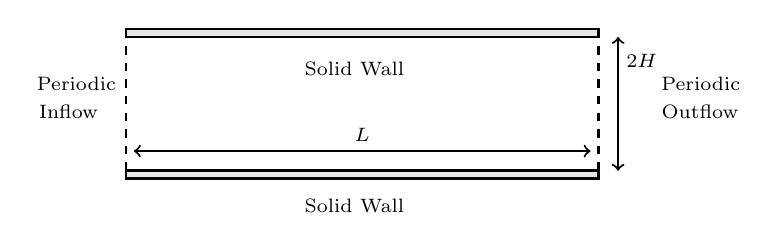
\begin{tikzpicture}
    % Draw a rectangle with specified properties
    \draw[line width=1pt, fill=gray!20] (0.0,1.8) rectangle (6.0,1.9);
    \draw[line width=1pt, fill=gray!20] (0.0,0.0) rectangle (6.0,0.1);
    \draw[dashed, line width=1pt] (0,0.1) -- (0,1.9);
    \draw[dashed, line width=1pt] (6,0.1) -- (6,1.9);
    
    \node at (2.6+0.3, 1.4) {\scriptsize Solid Wall};
    \node at (2.6+0.3, -0.35) {\scriptsize Solid Wall};
    
    \node at (-0.63, 1.2) {\scriptsize Periodic};
    \node at (-0.73, 0.85) {\scriptsize Inflow};
    
    \node at (7.15+0.15, 1.2) {\scriptsize Periodic};
    \node at (7.15+0.14, 0.85) {\scriptsize Outflow};
    
    % draw arrows
    \draw[<->, line width=0.75pt] (0.1, 0.35) -- (5.9, 0.35);
    \node at (3.0, 0.55) {\scriptsize $L$};
    \draw[<->, line width=0.75pt] (6.25, 0.1) -- (6.25, 1.8);
    \node at (6.55, 1.5) {\scriptsize $2H$};
    \end{tikzpicture}
    \captionsetup{width=0.85\textwidth}
    \caption{Computational domain for turbulent channel flow.}
    \label{fig:fully_developed_turbulent_channel_flow}
\end{figure}
The simulation is run at a Reynolds number $\text{Re}_H = 22000$ based on the half-channel height $H$.
However, in turbulence modelling and especially for turbulent channel flow, the friction Reynolds number ($\text{Re}_\tau $) given by $\text{Re}_\tau := (U_\tau H) / \nu $ is often used as a measure of the flow.
The simulation is run at $\text{Re}_\tau = 550$.
\begin{table}
    \centering
    \begin{tabular}{m{2.1cm} m{1.75cm} m{1.75cm} m{1.75cm} m{1.75cm}}
        \hline
        & $\mathbf{u}$ & $p$ & $k$ & $\varepsilon$ \\
        \hline
        \textbf{Inflow} & Periodic & $p=p_{\text{in}}$ & Periodic & periodic \\
        \textbf{Outflow} & Periodic & $p=p_\text{out}$ & Periodic & periodic \\
        \textbf{Solid walls} & $0$ & $\nabla p \cdot \mathbf{n} = 0$ & $0$ & $\nabla \varepsilon \cdot \mathbf{n} = 0$ \\
        \hline
    \end{tabular}
    \captionsetup{width=0.85\textwidth}
    \caption{Boundary conditions for turbulent channel flow.}
    \label{fig:fully_developed_turbulent_channel_flow}
\end{table}
To verify the model's accuracy, numerical results are compared to a direct numerical simulation performed by \cite{lee_direct_2015}.
The same simulation is conducted for a series of meshes with various values of $d^+$ ranging from $16$ to $0.5$ (with smaller values indicating a finer mesh), with the results provided in \cref{fig:channel_flow_profiles} (for better clarity, the results corresponding to some values of $d^+$ are not shown).
\begin{figure}[htbp]
    \centering
    \includegraphics[width=0.825\textwidth]{channel flow-profiles.pdf}
    \captionsetup{width=0.85\textwidth}
    \caption{Comparison of velocity (top) and turbulent kinetic energy (bottom) profiles obtained on meshes with different resolutions with direct numerical simulation (left), together with close-up plots (right).}
    \label{fig:channel_flow_profiles}
\end{figure}
Considering the solution profiles from \cref{fig:channel_flow_profiles} and the fact that the fields are most sensitive in the viscous sublayer, we feel that a value of $d^+ = 2$ strikes a good balance between computational efficiency and numerical accuracy.
In particular, the number of elements in this mesh is $864$.
The velocity and pressure spaces have $3,480$ and $511$ degrees of freedom, respectively. On the other hand, both the $k$ and $\varepsilon$ function spaces have $438$ degrees of freedom.
Since the results for meshes with values $d^+ = 2$ and $d^+ = 0.5$ do not differ dramatically, the former value will also be used when constructing a mesh for the next flow case.

\subsection{Flow over a Backward-Facing Step}
Flow over a backward-facing step occurs when a fluid flows over a sudden expansion, creating a separated flow region and a complex recirculation zone downstream of the step.
The domain and boundary conditions are constructed such that they match the data from the experiment performed by \cite{driver_features_1985}, which can be seen in \cref{fig:backward_facing_step} and \cref{tab: boundary conditions for the backward facing step}, respectively.
This is a significantly more complex scenario than the channel flow, making it a perfect model validation case.
Because of the mesh size, a steady-state solver was used.
\begin{figure}[htbp]
    \centering
    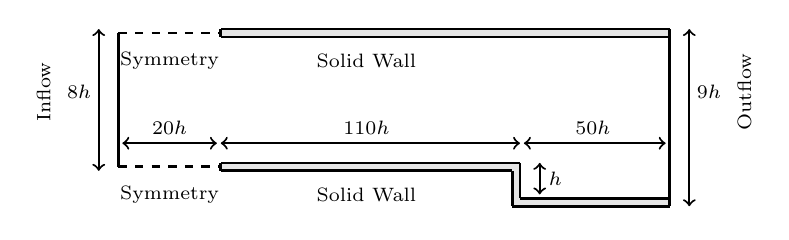
\begin{tikzpicture}
    
        \fill[gray!20] (2.3,1.7) rectangle (8.0,1.8);
        \draw[solid,  line width=1pt]     (2.3,1.7) -- (8.0,1.7);
        \draw[solid,  line width=1pt]     (8.0,1.7) -- (8.0,1.8);
        \draw[solid,  line width=1pt]     (8.0,1.8) -- (2.3,1.8);
        \draw[solid,  line width=1pt]     (2.3,1.8) -- (2.3,1.7);
        
        \fill[gray!20] (2.3,0.0) rectangle (6,0.1);
        \fill[gray!20] (6,-0.45) rectangle (8,-0.35);
        \fill[gray!20] (6,-0.45) rectangle (6.1,0.1);

        \draw[solid,  line width=1.0pt]     (2.3,0.0) -- (6.0,0.0);
        \draw[solid,  line width=1.0pt]     (6.0,0.0) -- (6.0, -0.45);
        \draw[solid,  line width=1.0pt]     (6.0, -0.45) -- (8.0, -0.45);
        \draw[solid,  line width=1.0pt]     (8.0, -0.45) -- (8.0, -0.35);
        \draw[solid,  line width=1.0pt]     (8.0, -0.35) -- (6.1, -0.35);
        \draw[solid,  line width=1.0pt]     (6.1, -0.35) -- (6.1, 0.1);
        \draw[solid,  line width=1.0pt]     (6.1, 0.1) -- (2.3, 0.1);
        \draw[solid,  line width=1.0pt]     (2.3, 0.1) -- (2.3, 0.0);

        \draw[dashed, line width=1pt]     (1.,1.75) -- (2.3,1.75);
        \draw[dashed, line width=1pt]     (1.,0.05) -- (2.3,0.05);
        \draw[solid,  line width=1pt]     (1.,0.05) -- (1.,1.75);
        \draw[solid,  line width=1pt]     (8,-0.35) -- (8,1.7);

        % Add text labels
        \node at (2.15+2.0, 1.4) {\scriptsize Solid Wall};
        \node at (2.15+2.0, -0.3) {\scriptsize Solid Wall};
        \node at (1.65, 1.4) {\scriptsize Symmetry};
        \node at (1.65, -0.3) {\scriptsize Symmetry};

        \node[rotate=90] at (0.05, 1.) {\scriptsize Inflow};
        \node[rotate=90] at (8.95, 1.) {\scriptsize Outflow};
        % draw arrows
        \draw[<->, line width=0.75pt] (6.35, 0.1) -- (6.35, -0.3);
        \node at (6.55, -0.1) {\scriptsize $h$};
 
        \draw[<->, line width=0.75pt] (1.05, 0.35) -- (2.25, 0.35);
        \node at (1.65, 0.55) {\scriptsize $20h$};
        
        \draw[<->, line width=0.75pt] (2.3, 0.35) -- (6.1, 0.35);
        \node at (4.15, 0.55) {\scriptsize $110h$};
        
        \draw[<->, line width=0.75pt] (6.15, 0.35) -- (7.95, 0.35);
        \node at (7.025, 0.55) {\scriptsize $50h$};

        \draw[<->, line width=0.75pt] (8.25, -0.45) -- (8.25, 1.8);
        \node at (8.5, 1.) {\scriptsize $9h$}; 
    
        \draw[<->, line width=0.75pt] (0.75, 0.0) -- (0.75, 1.8);
        \node at (0.5, 1.) {\scriptsize $8h$};
    \end{tikzpicture}
    \captionsetup{width=0.85\textwidth} 
    \caption{Computational domain for the flow over a backward-facing step.}
    \label{fig:backward_facing_step}
\end{figure}
The Reynolds number based on the step height $h$ is approximately $\text{Re}_h = 36,000$, where the reference velocity used to compute $\text{Re}_h$ is measured just before encountering the step, specifically at $x = -4h$ (with the step located at $x=0$).
The computational mesh consists of $129,844$ elements.
There are $523,038$ and $65,838$ degrees of freedom for the velocity and pressure spaces, respectively, and $65,838$ for both the $k$ and $\varepsilon$ spaces.
\begin{table}
    \centering
    \begin{tabular}{m{2.1cm} m{1.75cm} m{1.75cm} m{1.75cm} m{1.75cm}}
        \hline
        & $\mathbf{u}$ & $p$ & $k$ & $\varepsilon$ \\
        \hline
        \textbf{Inflow} & $\mathbf{u}_{\text{in}}$ & $\nabla p \cdot \mathbf{n} = 0$
        & $k_{\text{in}}$ & $\varepsilon_{\text{in}}$
        \\
        \textbf{Outflow} & $\nabla \mathbf{u} \cdot \mathbf{n} = 0$ & $p=0$
        & $\nabla k \cdot \mathbf{n} = 0$ & $\nabla \varepsilon\cdot \mathbf{n} = 0$
        \\
        \textbf{Solid walls} & $0$ & $\nabla p \cdot \mathbf{n} = 0$
        & $0$ & $\nabla \varepsilon \cdot \mathbf{n} = 0$
        \\
        \textbf{Symmetry} & $\mathbf{u} \cdot \mathbf{n} = 0$ & $\nabla p \cdot \mathbf{n} = 0$
        & $\nabla k \cdot \mathbf{n} = 0$ & $\nabla \varepsilon \cdot \mathbf{n} = 0$
        \\
        \hline
    \end{tabular}
    \captionsetup{width=0.85\textwidth}
    \caption{Boundary conditions for the flow over a backward-facing step.}
    \label{tab: boundary conditions for the backward facing step}
\end{table}

The model's accuracy is verified using experimental data from \cite{driver_features_1985}.
A key measure of success is the accurate prediction of the reattachment point downstream of the step.
This is determined by measuring the point $\hat{x}$ where the skin friction coefficient ($C_f$) is equal zero.
This was achieved in the experiment by using a laser oil flow interferometer. Another measure for analysing the results is the pressure coefficient ($C_p$).
The results in \cref{fig:backstep_coefficients} show a poor match between the simulation and the experiment, with the reattachment point observed at $\hat{x} = 6.26 h$, compared to the simulation's $\hat{x} = 5.0 h$.
However, this discrepancy is expected from the $k$-$\varepsilon$ model, which is known to struggle with separation and adverse pressure gradients.
When compared to results in \cite{steffen_jr._critical_1993} with multiple versions of the $k$-$\varepsilon$ model, with reattachment points ranging from $\hat{x} = 4.9$ to $\hat{x} = 5.5$, we see a better match.

\begin{figure}[htbp]
    \centering
    \includegraphics[width=0.825\textwidth]{backstep-coefficients.pdf}
    \captionsetup{width=0.85\textwidth}
    \caption{Comparison of the skin friction coefficient (left) and the pressure coefficient (right) between the experiment and simulation.}
    \label{fig:backstep_coefficients}
\end{figure}

\Cref{fig:backstep_profiles} presents normalized velocity magnitude $U/U_\infty$ and $k$ profiles at four points after the step.
Although the velocity profiles show good agreement, $k$ diverges after $x = 4h$, which is likely the cause of the reattachment point appearing prematurely.
\begin{figure}[htbp]
    \centering
    \includegraphics[width=0.825\textwidth]{backstep-profiles.pdf}
    \captionsetup{width=0.85\textwidth}
    \caption{Comparison of the velocity (top) and turbulent kinetic energy (bottom) profiles at $x = 1h$ (left), $x = 4h$ (second left), $x = 6h$ (second right), and $x = 10h$ (right) between the experiment and simulation.}
    \label{fig:backstep_profiles}
\end{figure}

% Section 4 - Conclusion
\section{Conclusion}
The LB $k$-$\varepsilon$ turbulence model was successfully implemented on the FEniCS computing platform, in both the transient and steady-state formulations.
We verified the implementation of the transient solver by simulating fully developed channel flow, where very good agreement was found between the computed solutions and the direct numerical simulation.
Although the results of the backward-facing step simulation did not match the experiment, we still consider the implementation of the steady-state solver a success, since the results matched the expected behaviour of the $k$-$\varepsilon$ model.
It is clear from those results that the working $k$-$\varepsilon$ model in FEniCS can be implemented with relative ease, and we see no reason why that would not be true for different turbulence models such as the $k$-$\omega$ or Spalart--Allmaras model.
These results can be replicated via scripts archived at \href{https://github.com/joove123/k-epsilon}{https://github.com/joove123/k-epsilon}.

\begin{acknowledgement}
    I would like to thank my master's thesis supervisor, Professor Achim Schroll, for professional guidance and support during the writing of my master's thesis and this article.
    I also thank NumFOCUS for the travel award that enabled me to attend the FEniCS 2024 conference.
\end{acknowledgement}
% ---- Article ends here ----
\bibliographystyle{spbasic}
% Write the full path of your bibfile relative to book.tex
\bibliography{chapters/marcibal/bibliography.bib}


\graphicspath{{chapters/munthe/graphics/}}


\title{Growth and Remodelling Package in FEniCSx}

\author{Karl Munthe, Henrik N.T. Finsberg, Samuel T. Wall, and Joakim Sundnes}

\institute{K. Munthe \email{karlfredrik@simula.no} \at Simula Research Laboratory, Oslo, Norway and \\ Department of Informatics, University of Oslo, Norway 
\and
H. Finsberg \at Simula Research Laboratory, Oslo, Norway
\and
S. Wall \at Simula Research Laboratory, Oslo, Norway
\and
J. Sundnes \at Simula Research Laboratory, Oslo, Norway, and \\ Department of Informatics, University of Oslo, Norway}

\maketitle
\abstract{The heart is a dynamic organ that changes its size and shape to regulate its behaviour to the demands of the body, which can change, for example, through body growth, exercise, or the onset of disease. Different models have been proposed to capture various types of cardiac growth resulting from mechanical stimuli, but the models have rarely been compared systematically. In this manuscript, we present a framework implemented in FEniCSx that allows one to quickly run simulations of growth and remodelling with different material models and different growth laws. We present and compare the growth predicted by each model for a set of simple experiments and compare the results to the literature. All the code can be found at \url{https://github.com/karlfm/Growth-and-Remodeling-in-FEniCSx}.}
\vspace{12pt}
\section{Introduction}
In classical continuum mechanics, one normally studies the mechanics of bodies where mass, linear momentum, angular momentum, and energy are conserved. This approach has been extremely successful and is the bedrock for traditional engineering disciplines, but it does not accurately capture aspects of how living organisms change with respect to their environment. One of the unique features of biological material is its ability to grow and evolve by adding or removing mass. Understanding how biological matter grows and what drives the growth is important, not only to understand normal growth and development but also when and how growth can become non-compensatory and drive disease.\par It has been known for a long time that the growth of organs, such as the heart, is regulated at least partly by the forces applied to it \citep{Hsu1968}. This understanding has led to the formulation of growth laws that link growth and remodelling to local stress or strain. \par
In this chapter, we introduce a package written in FEniCSx that allows one to easily model the growth and remodelling of biological tissue, with the aim of quickly testing combinations of growth models and material models. Allowing researchers to systematically test combinations of material models and growth tensors will aid in the discovery of more accurate models of growth and remodelling phenomena of biological tissue.
\section{Methods}
\subsection{Growth and Remodelling in Continuum Mechanics}
Consider a solid body that is continuously and smoothly deforming from one configuration to another and denote the initial configuration (also called the reference configuration) as $\mathcal{M}$ and the current configuration as $\mathcal{N}$. We denote a point in $\mathcal{M}$ with uppercase letters $\mathbf{X} = (X, Y, Z)$ and a point in $\mathcal{N}$ with lowercase letters $\mathbf{x} = (x, y, z)$\footnote{Apart from the letters $X$, $Y$, and $Z$, all uppercase letters represent tensors.}. A point in $\mathcal{M}$ can be mapped to a point in $\mathcal{N}$ by a motion $\phi(\mathbf{X}): \mathbf{X} \rightarrow \mathbf{x}$, which is a diffeomorphism. We can map a vector from the reference configuration to the current configuration via the pushforward of $\phi$, which is commonly denoted by $\mathbf{F}$ and is referred to as the deformation gradient, computed as $\mathbf{F} = \partial\mathbf{x}/\partial\mathbf{X}$. The displacement field $\mathbf{u} = \mathbf{x} - \mathbf{X}$ is a vector field describing the displacement of each point $\mathbf{X}$ in the reference configuration to its location $\mathbf{x}$ in the deformed configuration. 
Most mechanical models of the heart assume that the tissue is hyperelastic, meaning that deformations of the material conserve their energy, and when any load on the tissue is removed, the material returns to its original reference shape. Growth, on the other hand, represents a permanent change of the unloaded reference configuration and cannot be modelled as an elastic deformation. Instead, it is commonly modelled using the framework of plastic or elastoplastic deformations. The most common approach, introduced by \cite{Rodriguez1994}, is to multiplicatively split the deformation tensor into an elastic part and an inelastic growth part, 
\begin{equation}
\label{eq: multiplicative split}
    \mathbf{F} = \mathbf{F}_e\mathbf{F}_g,
\end{equation}
where $\mathbf{F}_e$ is the elastic deformation and $\mathbf{F}_g$ is the plastic deformation that represents growth. 

One interpretation of \ref{eq: multiplicative split} is that the material first deforms by $\mathbf{F}_g$ in a way that does not cause stress but might cause incompatibilities in the form of discontinuities or overlapping material. The deformation described by $\mathbf{F}_g$ leads to an unphysical intermediate configuration, which is then deformed by $\mathbf{F}_e$ in a way that removes the unphysical characteristics that resulted from $\mathbf{F}_g$ but adds residual stress. Sufficient conditions for the existence of intermediate configurations such as $\mathbf{F}_g$ are discussed in \cite{Goodbrake2021}. We assume that the deformation described by $\mathbf{F}_e$ is hyperelastic such that we can obtain the first Piola–-Kirchhoff stress tensor by differentiating a strain energy function,
\begin{equation}
\label{eq: stress}
    \mathbf{P} = \frac{\partial\Psi}{\partial \mathbf{F}_e}.
\end{equation}

We typically describe the growth in terms of multiple growth steps, given by
\begin{equation*}
    \mathbf{F}_g^{i + 1} = \mathbf{F}_g^i\mathbf{F}_g^\mathrm{inc},
\end{equation*}
where $\mathbf{F}_g^\mathrm{inc}$ is the incremental growth tensor describing the growth occurring in one step and $\mathbf{F}_g^i$ is the cumulative growth after $i$ steps. The initial growth tensor, $\mathbf{F}_g^0$, is set to the identity tensor. The cumulative growth deformation tensor after $n$ steps is given by
\begin{equation*}
    \mathbf{F}_g^{n} = \mathbf{F}_{g}^\mathrm{inc}\vert_{t=0}\mathbf{F}_{g}^\mathrm{inc}\vert_{t=1} \cdots \mathbf{F}_{g}^\mathrm{inc}\vert_{t=n},
\end{equation*}  
where $\mathbf{F}_{g}^\mathrm{inc}\vert_{t=i}$ means $\mathbf{F}_{g}^\mathrm{inc}$ at the $i$th step. Note that the $i$th incremental growth tensor is dependent on the stress or strain that occurred in the ($i-1$)th growth step \citep{Goriely2007}. It is common to assume that the growth tensor is diagonal and to express the incremental growth tensor in terms of fibre, cross-fibre, and normal directions: 
\begin{equation*}
    \mathbf{F}_g^\mathrm{inc} = F^\mathrm{inc}_{g,f}\mathbf{e}_f\otimes \mathbf{e}_f + F^\mathrm{inc}_{g,c}\mathbf{e}_c\otimes \mathbf{e}_c + F^\mathrm{inc}_{g,n}\mathbf{e}_n\otimes \mathbf{e}_n,
\end{equation*}
where the $F^\mathrm{inc}_{g, i}$ terms for  $i = \{f, c, n\}$ are functions of either stress or strain, and the $\mathbf{e}_i$ terms for $i = {\{f, c, n\}}$ are orthonormal basis vectors in the fibre, cross-fibre, and normal directions, respectively. 

The incremental growth tensor depends on the local stress or strain, which is determined by solving for mechanical equilibrium at each growth step: 
\begin{equation} \label{eq: system of equations}
\begin{aligned}
    \mathbf{F} & = \mathbf{F}_e\mathbf{F}_g && \text{in } \mathcal{M} ,\\
    \nabla\cdot\mathbf{P} & = 0 && \text{in } \mathcal{M}, \\
    \mathbf{P}\cdot \nu & = 0 && \text{on } \partial\mathcal{M}_N, \\
    \mathbf{u} & = g_D && \text{on } \partial\mathcal{M}_D,
\end{aligned}
\end{equation} 
where $\nu$ is a surface normal vector, and $\partial\mathcal{M}_N$ and $\partial\mathcal{M}_D$ denote the boundaries that are prescribed Neumann and Dirichlet boundary conditions, respectively. 

The growth laws that determine $F_g$ and the strain energy $\Psi$ in 
(\ref{eq: stress}) still need to be specified. We will define the growth laws in the next section, but we use a nearly incompressible neo-Hookean model for all the 
experiments, so (\ref{eq: stress}) becomes
\begin{align*}
    \mathbf{P} &= \frac{\partial\Psi_\text{iso}}{\partial \mathbf{F}_e} + \frac{\partial\Psi_\text{vol}}{\partial \mathbf{F}_e}, \\
    \mathbf{P} &= \frac{\partial}{\partial \mathbf{F}_e}\left[\frac{\mu}{2}\left(\mathrm{tr}\mathbf{\bar{C}} - 3\right) + \kappa(J-1)^2\right],
\end{align*}
where $\mu$ and $\kappa$ are material parameters, and $\Psi_\text{iso}$ and $\Psi_\text{vol}$ are the isochoric (distortional) and volumetric (dilational) parts of the strain energy function, respectively. To decouple the energy stored in the body as a result of volume-preserving deformation and non--volume-preserving deformation, we introduce $\mathbf{\bar{F}}_e = \mathbf{F}_eJ^{-1/3}$, whose determinant is equal to one. The isochoric right Cauchy--Green deformation tensor, $\mathbf{\bar{C}}$, is calculated as $\mathbf{\bar{C}} = \mathbf{\bar{F}}_e^\top \mathbf{\bar{F}}_e$. Now, $\partial\Psi_\text{iso}/\partial \mathbf{F}_e = 0$ only if the deformation preserves the shape, and $\partial\Psi_\text{vol}/\partial \mathbf{F}_e = 0$ only if the deformation preserves the volume (for more details, see Chapter 6 of \cite{Holzapfel2002}). \par 
For further information about continuum mechanics, we recommend \cite{Marsden1983} and \cite{Holzapfel2002}, and for further information about growth and remodelling, we recommend \cite{Goriely2017} and \cite{Yavari2010}.

\subsection{Numerical Implementation}
 
Algorithm \ref{alg:growth_deform} gives an overview of the steps involved in the solution
of the growth model equations. For stress-based growth, one would update the stress tensor rather than the strain tensor, and for additive growth laws, one would sum the cumulative and incremental growth tensors instead of multiplying them. \par
\begin{algorithm} 
    \caption{The growth tensor and stress/strain tensor are updated at each growth step. Both $\mathbf{F}_\mathrm{e}$ and $\mathbf{F}_g^\mathrm{inc}$ are dependent on $\mathbf{u}$.}\label{alg:growth_deform}
    \SetAlgoLined
    \For{each time step}{
        Solve (\ref{eq: system of equations}) for the displacement $\mathbf{u}$\;
        Update the stress/strain tensor using the obtained displacement $\mathbf{u}$.\;
        Update the growth tensor using the stress/strain tensor from the previous line.\;
    }
\end{algorithm} 
\emph{Constructing the weak form}: We multiply $\nabla\cdot\mathbf{P}$ by a test function, which we set to be in the same function space as $\mathbf{u}$, and integrate over a discretization of $\mathcal{M}$. By applying integration by parts, we obtain
\begin{align}
    \label{eq: weak conservation of momentum}
    \int_\Omega(\nabla\cdot\mathbf{P})\cdot\eta d\mathbf{X} &= 0  \notag\\
    \int_\Omega \mathbf{P} : \nabla\eta d\mathbf{X} &= \int_{\partial\Omega}\mathbf{P}\cdot\eta \cdot \nu dA.
\end{align}
Since we are using test functions $\eta$ that vanish on $\partial_D\mathcal{M}$ and the normal component of $\mathbf{P}$ is zero on $\partial_N\mathcal{M}$, we can set the boundary integral to zero. Then (\ref{eq: weak conservation of momentum}) is solved using FEniCSx \citep{DOLFINx}. 
\par
\emph{Iteratively solving the conservation of momentum}: We now solve (\ref{eq: weak conservation of momentum}) for the displacement $\mathbf{u}$, which we can use to compute all the necessary variables. We use tetrahedral, second-order, continuous Lagrange elements to approximate $\mathbf{u}$, and first-order, discontinuous Lagrange elements to approximate $\mathbf{F}_e$ and $\mathbf{F}_g$. This is a common numerical scheme in cardiac mechanics that has been demonstrated to avoid locking \citep{oliveira2016comparison}. 

\subsection{Solving Growth Laws on the Unit Cube}
\label{subsec: simulations}
In the simulations we have run, we have aligned the $x$-axis with the fibre direction, with the $y$- and $z$-axes as the cross-fibre and normal directions, respectively. For consistency with the literature, we use $\mathbf{e}_f$, $\mathbf{e}_c$, and $\mathbf{e}_n$ to denote the unit vectors in the $(x, y, z)$ directions, respectively.  \par
\emph{Boundary conditions:} We set the following boundary conditions:
\begin{align*}
    g_D = \begin{cases}
        u &= \begin{cases}
            0 & \text{on } x = 0, \\
            u_D & \text{on } x = 1,
        \end{cases} \\
        v &= 0 \qquad \ \ \text{on } y = 0, \\
        w &= 0 \qquad \ \ \text{on } z = 0,
    \end{cases}
\end{align*}
where $u$, $v$, and $w$ are the displacement in the $x$, $y$, and $z$ directions, respectively, and $u_D$ specifies by how much the body is displaced. 
\par

\emph{Numerical simulations:} We ran two simulations, one with a 10\% stretch and one with a 10\% compression, corresponding to $u_D = 0.1$ and $u_D = -0.1$, respectively. For the GCG model, $F_{g,c,\mathrm{max}}$ was set to 1.2 in the stretch simulation and 0.8 in the compression simulation (see Table \ref{tab:growth models}). We set $\mu = 15$ kPa and $\kappa = 100$ kPa.
\subsection{Growth Models}
\label{sub:different models} 
In this paper, we compare five growth models that we have taken from \cite{Taber1998}, \cite{Kroon2009}, \cite{Goktepe}, and \cite{Kerckhoffs2012}. The growth models are presented in Table \ref{tab:growth models}, where the LT2 model is from \cite{Taber1998}, the KFR model is from \cite{Kroon2009}, the GEG and GCG models are from \cite{Goktepe}, and the KOM model is from \cite{Kerckhoffs2012}. Each growth model has a set point that determined the homeostatic level of either stress, stretch, or strain. When the stress, stretch, or strain reaches the set point, growth will cease to occur. If this does not happen, the body will grow indefinitely, which we call runaway growth. We used the same variables as in the original works, except for the GCG model, where we scale the variables to more accurately fit the shear modulus used here. The values are tabulated in Table \ref{tab:parameters}.
%\newgeometry{right=1cm, left=1cm}%,right=1cm,top=1cm,bottom=1cm}
\begin{table}
\centering
\makebox[\textwidth][c]{
\renewcommand{\arraystretch}{4}
\begin{tabular}{|c||c|c|c|}
\hline \hline
 & $F_{g,f}^{i+1}$ & $F_{g,n}^{i+1}$ & $F_{g,c}^{i+1}$ \\
\hline \hline
LT2 & $\displaystyle F_{g,f}^i\left(\frac{\sigma_{\theta p} - \sigma_{p,0}}{T\sigma_{p,0}} + 1\right)$ & $\displaystyle F_{g,n}^i\left(\frac{\sigma_{\theta a} - \sigma_{a,0}}{T\sigma_{a,0}} + 1\right)$ & $\displaystyle 1$ \\
\hline
KFR & $\displaystyle F_{g,f}^i(\beta(\sqrt{2 E_{ff} + 1} - 1 - s_\mathrm{hom}) + 1)^{1/3}$ & $\displaystyle F_{g,n}^i(\beta(\sqrt{2 E_{ff} + 1} - 1 - s_\mathrm{hom}) + 1)^{1/3}$ & $\displaystyle F_{g,c}^i(\beta(\sqrt{2 E_{ff} + 1} - 1 - s_\mathrm{hom}) + 1)^{1/3}$ \\
\hline
GEG & $\displaystyle \frac{1}{\tau}\left(\frac{F_{g,f,\mathrm{max}} - F_{g,f}^i}{F_{g,f,\mathrm{max}} - 1}\right)^\gamma(F_{e, f}^i - \lambda^\text{crit}) + F^i_{g, f}$ & $\displaystyle 1$ & $\displaystyle 1$ \\
\hline
GCG & $\displaystyle 1$ & $\displaystyle  \frac{1}{\tau}\left(\frac{F_{g,c,\mathrm{max}} - F_{g,c}^i}{F_{g,c,\mathrm{max}} - 1}\right)^\gamma(\tr(\mathbf{M}) - p^\mathrm{crit}) + F^i_{g, c}$ & $\displaystyle 1$ \\
\hline
KOM & $\displaystyle \begin{cases}
        F_{g,f}^{i}k_{ff}\frac{f_\mathrm{ff, max}\Delta t_\text{growth}}{1 + \exp(-f_f(s_\mathrm{l}-s_{l,50}))} + 1, \qquad s_\mathrm{l} \geq 0\\
        F_{g,f}^{i}\frac{-f_\mathrm{ff, max}\Delta t_\text{growth}}{1 + \exp(f_f(s_\mathrm{l}+s_{l,50}))} + 1, \qquad s_\mathrm{l} < 0
    \end{cases} $ & $\displaystyle \begin{cases}
        F_{g,c}^{i}\sqrt{k_{cc}\frac{f_{cc,\mathrm{max}}\Delta t_\text{growth}}{1 + \exp(-c_\mathrm{f}(s_\mathrm{t}-s_{t,50}))} + 1}, \qquad s_\mathrm{t} \geq 0\\
        F_{g,c}^{i}\sqrt{\frac{-f_{cc,\mathrm{max}}\Delta t_\text{growth}}{1 + \exp(c_\mathrm{f}(s_\mathrm{t}+s_{t,50}))} + 1}, \qquad s_\mathrm{t} < 0 
    \end{cases} $ & $\displaystyle \begin{cases}
        F_{g,c}^{i}\sqrt{k_{cc}\frac{f_{cc,\mathrm{max}}\Delta t_\text{growth}}{1 + \exp(-c_\mathrm{f}(s_\mathrm{t}-s_{t,50}))} + 1}, \qquad s_\mathrm{t} \geq 0\\
        F_{g,c}^{i}\sqrt{\frac{-f_{cc,\mathrm{max}}\Delta t_\text{growth}}{1 + \exp(c_\mathrm{f}(s_\mathrm{t}+s_{t,50}))} + 1}, \qquad s_\mathrm{t} < 0 
    \end{cases} $ \\
\hline
\end{tabular}
}
\caption{The terms $F_{g,f}$, $F_{g,c}$, and $F_{g,n}$  for each of the five models. The parameters $T$, $\beta$, $\tau$, and $\Delta t$ simply determine the rate of growth and can be tuned to match the growth rate of the data obtained from experiments.}
\label{tab:growth models}
\end{table}
%\restoregeometry
\begin{table}[htbp]
    \centering
    \begin{tabular}{|l|l|}
    \hline
    \textbf{Model} & \textbf{Parameters} \\
    \hline
    \textbf{LT2} &   $\sigma_{a,0} = 30$ [kPa], $\sigma_{p,0} = 3$ [kPa], $T = 10^{-4}$ \\ \hline
    \textbf{KFR} &  $s_\mathrm{hom} = 0.13, \beta = 10^{-2}$ \\ \hline
    \textbf{GEG} &  $F_{g,f,\mathrm{max}}=1.5$, $\lambda^\mathrm{crit}=1.01$, $\gamma = 2$, $\tau = 10^2$ \\ \hline
    \textbf{GCG} &  $F_{g,c,\mathrm{max}}=1.2$ and $0.8$,  $p^\mathrm{crit}=0.12, \gamma = 2, \tau = 10^4$ \\ \hline
    \textbf{KOM} &  $f_\mathrm{ff,max} =0.31$ [1/days], $f_f = 150$, $s_{l50} = 0.06$, $F_{ff50} = 1.35$, $f_{l,\mathrm{slope}} = 40$, $f_\mathrm{ff,max} = 0.1$ [1/days] \\
        & $c_\mathrm{f} = 75$, $s_\mathrm{t50} = 0.07$, $F_\mathrm{cc50} = 1.28$, $c_\mathrm{th,slope} = 60$, $E_{ff,\mathrm{set}} = 0$, 
        $E_\mathrm{cross,\mathrm{set}} = 0$, $\Delta t = 10^{-2}$ [days] \\ \hline
    \end{tabular}
    \caption{Model parameters for the growth models. The terms $T$, $\beta$, $\tau$, and $\Delta t$ determine the speed of growth.}
    \label{tab:parameters}
\end{table}
In the LT2 model, $\sigma_{p,0}$ and $\sigma_{a,0}$ are set points for the passive and active fibre stresses at equilibrium, and $\sigma_{\theta p}$ and $\sigma_{\theta a}$ are the active and passive fibre stresses, respectively. In the simulations we have run, we have only used the passive component of $\sigma$ and have set $\sigma_a = 0$. For the KFR model, $s_\mathrm{hom}$ is the strain set point. For the GEG and GCG models, $F_{g,f,\mathrm{max}}$ and $F_{g,c,\mathrm{max}}$ are the maximum amounts of growth allowed to occur, respectively. The term $\mathbf{M}$ is the Mandel stress, which is defined as 
\begin{equation*}
    \mathbf{M} = \mathbf{F}^\top \mathbf{P},
\end{equation*}
and $p^\mathrm{crit}$ is the stress set point. The term $\lambda^\text{crit}$ is the strain set point. For the KOM model, $k_{ff}$ and $k_{cc}$ are defined as
\begin{align*}
    k_{ff} &= \frac{1}{1 + \exp(f_\text{length,slope}(\mathbf{F}_{g,ff}^i - F_{ff,50}))}, \\
    k_{cc} &= \frac{1}{1 + \exp(c_\text{thickness,slope}(\mathbf{F}_{g,cc}^i - F_{cc,50}))},
\end{align*}
and $s_\mathrm{l}$ and $s_\mathrm{t}$ are defined as
\begin{align*}
    s_\mathrm{l} &= \max(E_{ff}) - E_{ff, \mathrm{set}}, \\
    s_\mathrm{t} &= \min(E_\text{cross, max}) - E_\mathrm{cross, set},
\end{align*}
where $E_{ij}$ is the Lagrange strain tensor, $E_{ff}$ is the strain in the fibre direction, and $E_\text{cross, max}$ is the maximum algebraic maximum principal strain of the matrix \citep{Witzenburg2018}:
\begin{equation*}
    E_\text{cross} = \begin{pmatrix}
        E_{cc} & E_{cr} \\
        E_{rc} & E_{rr}
    \end{pmatrix},
\end{equation*}
and $E_{ff, \mathrm{set}}$ and $E_\mathrm{cross, set}$ are set points. \par
Growth stops for the LT2 model when $\sigma_{\theta} = \sigma_{0}$. For the KOM model, since $k_{cc}$ and $k_{ff}$ are logistic functions, growth is bounded from above and below, inhibiting runaway growth. Finally, for the KFR model, it does not appear obvious that it will not obtain runaway growth, and other simulations setups that were tested did result in runaway growth, even though the one we present here does not.

\section{Results}
The data we collected from the simulations described in Section \ref{subsec: simulations} were the stretch and growth that occurred in the middle of the cube. The results are depicted in Figs. \ref{fig:10p_stretch} and \ref{fig:10p_compression}. The top row of each figure displays the fibre and cross-fibre components of the growth tensor, $\mathbf{F}_g$, and the bottom row displays the fibre and cross-fibre components of the elastic deformation tensor, $\mathbf{F}_e$. In the simulations we ran, $\mathbf{F}_e$ is diagonal, so the components of $\mathbf{F}_e$ are the principal stretches. This is because $\sqrt{\mathbf{e}_i^\top\mathbf{C}_e\mathbf{e}_i}$ is the principal stretch in the $i$th direction, and $\sqrt{\mathbf{e}_i^\top\mathbf{C}_e\mathbf{e}_i} = \sqrt{\mathbf{e}_i^\top\mathbf{F}_e^\top\mathbf{F}_e\mathbf{e}_i} = \mathbf{F}_e\mathbf{e}_i$. By the same reasoning, the diagonal components of $\mathbf{F}_g$ (which are the only nonzero components), denote the growth in the fibre, cross-fibre, and normal directions. Increasing $\kappa$ did not yield qualitatively different results. \par
The GCG model seems to be converging to $F_{g,c,\mathrm{max}}$, and the GEG model seems to have converged because it reached $\lambda^\text{crit}$. The reason the GCG model is showing growth oppositely compared to the GEG model is probably because the GEG model was created to model growth triggered by volume overload, whereas the GCG model was created to capture growth triggered by pressure overload. The KFR model showed equal amounts of growth in each direction and stabilized. It is not clear under what conditions the KFR model should be stable, because $s_\mathrm{hom}$ is the same in each direction. When we ran simulations with other boundary conditions, the solution diverged. The KOM model was stable for many different types of boundary conditions, but it is the most computationally expensive to run.\par 
\begin{figure}[h]
    \centering
    \includegraphics[width=\textwidth]{10p_stretch_3.png}
    \caption{Growth and stretch predicted by 10\% stretch in the fibre direction}
    \label{fig:10p_stretch}
\end{figure}
\begin{figure}[h]
    \centering
    \includegraphics[width=\textwidth]{10p_compression_3.png}
    \caption{Growth and stretch predicted by 10\% compression in the fibre direction}
    \label{fig:10p_compression}
\end{figure}    

\section{Conclusion and Future Work}
We have implemented a general growth and remodelling framework using the FEniCSx program in Python. The goal is to easily change material models and growth models. This will allow researchers to compare their models with other models in the field. Future work will include the implementation of more complex geometries, more growth laws, and more material models. The models we have used in this chapter are not derived from the dissipation equation but are, instead, phenomenologically derived growth laws, and future work should investigate whether they satisfy the laws of thermodynamics. Another avenue of future research we wish to pursue is examining constrained mixture models, which model how changes in various constituents influence the characteristics of tissue. We also wish to add models that have more mathematically sophisticated stopping criteria, such as those developed by \cite{Erlich2023}. The authors use an energy penalty to construct a stopping criterion, and \cite{Erlich2024} look into how curvature\footnote{The intrinsic three-dimensional curvature, not the two-dimensional curvature of the surface of the body.} in the reference configuration could be used as a stopping criterion. Future work will also implement the growth models on geometries with fibres. We tried running the models on various fibre orientations and found them to be extremely sensitive to fibres that varied throughout the domain. Preliminary results indicate that some of the models do not converge to a steady state for relatively small perturbations of the variables or if the fibres are not well aligned with the body, something we plan on quantifying in the future. \par

When this package is further developed, we aim to add it to the Pulse package. \footnote{See https://github.com/finsberg/fenicsx-pulse.} \par
The models we compared were developed to capture different aspects of growth and were tuned to be used on different material models. An apples-to-apples comparison might therefore be unfair. Furthermore, the growth models we used do not take into account residual stresses that exist within the material before or after growth. \par
Finally, experimental data are needed to verify which models are accurate or to capture the correct phenomena of growing cardiac tissue.
% \newpage
\bibliographystyle{spbasic}
\bibliography{chapters/munthe/bibliography.bib}
% \printbibliography
% \end{document}




\title{Blood Flow in the Beating Heart: Coupling Fluid Dynamics to Reduced Wall and Circulation Models for Data-Driven Cardiac FSI}
\titlerunning{Blood Flow in the Beating Heart}

\author{Marc Hirschvogel, Mia Bonini, Maximilian Balmus, and David Nordsletten}
\authorrunning{Hirschvogel et al.}

\institute{Marc Hirschvogel \email{marc.hirschvogel@polimi.it} \at MOX, Mathematics Department, Politecnico di Milano, Milan, Italy}

\maketitle

\abstract{We present a fluid--reduced solid interaction approach suitable for modelling blood flow in a beating left heart. 
The method uses image-derived model data to construct a suitable boundary motion space enhanced by a reduced solid mechanics wall model to enable adaptive fluid motion. 
The method combines the efficiency of fluid dynamics models with features from full fluid--solid interaction approaches, uniquely integrating motion data to predict cardiac haemodynamics over a full heart cycle. 
The approach is presented for a patient-specific left heart model coupled to a lumped circulatory system, showing physiological flow behaviour and pressure--volume relations.}


\section*{Introduction}
Computational fluid dynamics (CFD) provides a valuable tool to predict blood flow in the cardiovascular system \citep{schwarz2023}. 
Models of blood flow in the heart have become relevant to predict various cardiovascular conditions, using motion states from imaging \citep{bonini2022-suppl,zingaro2023,garciavillalba2021} or even fully coupled fluid--solid interaction (FSI) models \citep{nordsletten2011-fsi,mccormick2011modelling}. 
However, prescribed cavity motion reduces the model's ability to adapt under varying loads, and full FSI models are complex, computationally demanding, and difficult to constrain (with uncertain boundary conditions and sparse patient data for reliable geometry reconstruction).
The fluid--reduced solid interaction (FrSI) method closes the gap between model complexity and efficiency. This is a data-informed model reduction approach, particularly suited for cardiac FSI \citep{hirschvogel2024-frsi}. 
The method combines physics with projection-based model reduction techniques that leverage proper orthogonal decomposition (POD) modes derived from imaging (or some high-fidelity model) to build a reduced-order model (ROM) combined with a structural model of the ventricular wall defined on a 2D manifold.
In this contribution, we show the FrSI method's applicability to a complex patient-specific left heart model, with particular focus on monolithic solver implementations in FEniCSx \citep{alnaes2015fenics, baratta2023dolfinx}. This method encompasses the implementation of an arbitrary Lagrangian--Eulerian (ALE) fluid mechanics problem subject to nonlocal constraints (Galerkin ROM, 3D--0D coupling to lumped circulation models). 
The solver and preconditioning aspects of this model and other fluid dynamics problems under nonlocal boundary conditions have been introduced in \cite{hirschvogel2025-prec}.


\section*{Methods}
The FrSI problem of a 3D left heart model (atrium, ventricle, aortic outflow tract) along with the underlying data sources is depicted in \Cref{fig:heart_problem}. 
In particular, domain and motion data are retrieved from time-resolved dynamic CT, which are subsequently mapped to a finite element mesh to generate a discrete space of modes using POD \citep{rathinam2003}. 
The model is further coupled to a closed-loop systemic, pulmonary, and coronary circulation system \citep{hirschvogel2017,arthurs2016} to provide physiologically meaningful cardiovascular loads to the 3D model.
\begin{figure}[!htp]
\centering
\includegraphics[width=1\textwidth]{chapters/hirschvogel/heart_problem.pdf}

\caption{FrSI problem of a 3D left heart model, with underlying data sources. 
\textbf{A.} Dynamic cardiac computed tomography (CT) images with contrast and dynamic segmentation of left heart lumen for subsequent finite element mesh generation, with motion tracking of deformation over the heart cycle. 
\textbf{B.} Principal component analysis of wall motion space by means of POD, showing the first three dominant POD modes (10 are used). 
\textbf{C.} Partition of unity fields for the regional decomposition of POD space: atrium, ventricle, and aortic outflow tract -- as well as their junctions and truncations around in-/outflows -- can exhibit independent kinematics. 
\textbf{D.} 3D--0D coupled FrSI model of the left heart.}\label{fig:heart_problem}
\end{figure}

\subsection*{Patient Data Preprocessing }
The FrSI approach relies on external data sourced from either some high-dimensional model or patient-specific imaging data. Here, we build a patient-specific model of the left heart by segmenting a dynamic cardiac CT dataset using 3D Slicer \citep{kikinis2014-3dslicer}; see \Cref{fig:heart_problem}A. A diastolic frame is subsequently meshed with SimModeler \citep{simmodeler}, and a motion tracking algorithm is used to extract the wall velocities at each frame and map them to the finite element mesh (with a velocity degree-of-freedom space of size $n_{v}$). Thereafter, the wall velocity data for $m=19$ frames is collected into a snapshot matrix $\hat{\boldsymbol{\mathsf{S}}} \in \mathbb{R}^{n_{v} \times m}$, and the eigenvalue problem
\begin{align}
    (\hat{\boldsymbol{\mathsf{S}}}^{\mathrm{T}} \hat{\boldsymbol{\mathsf{S}}}) \,\boldsymbol{\uppsi}_{i} = \uplambda_{i} \,\boldsymbol{\uppsi}_{i}, \quad i = 1, \hdots, m,\label{eq:rom_eigensolve}
\end{align}
is solved, with eigenvalues $\uplambda$ and eigenvectors $\boldsymbol{\uppsi} \in \mathbb{R}^{m}$. The first $r_{v}$ POD modes $\boldsymbol{\upphi} \in \mathbb{R}^{n_{v}}$ can then be computed as follows:
\begin{align}
    \boldsymbol{\upphi}_{j} = \frac{1}{\sqrt{\uplambda_{j}}} \hat{\boldsymbol{\mathsf{S}}} \boldsymbol{\uppsi}_{j}, \quad j = 1, \hdots, r_{v}, \label{eq:phi_Phi_frsi}
\end{align}
the first three of which are shown in \Cref{fig:heart_problem}B. A suitable Galerkin model reduction operator
\begin{align}
    \boldsymbol{\mathsf{V}}_{v}^{\Gamma} \in \mathbb{R}^{n_v \times (r_v + n_{v}^{\mathit{\Omega}})}, \label{eq:Vgamma}
\end{align}
then needs to be defined, with $n_{v}^{\mathit{\Omega}}$ as the size of the space of bulk (non-boundary) velocities. In \cref{eq:Vgamma}, POD modes \cref{eq:phi_Phi_frsi} have to be incorporated such that velocity degrees of freedom on $\Gamma_{0}^{\mathrm{f}\text{-}\tilde{\mathrm{s}}}$ are confined to the lower-dimensional subspace, but those associated with the bulk domain remain unconstrained \cite{hirschvogel2024-frsi}. Furthermore, the POD space is decomposed with a partition of unity approach such that each region can exhibit independent kinematics (see \cref{fig:heart_problem}C).

\subsection*{Strong Form Problem Statement}
We briefly state the strong problem of FrSI -- fluid dynamics in an ALE reference frame \citep{donea1982,duarte2004} with a reduced structural wall model -- subject to nonlocal flux-dependent tractions at the in- and outflows. The boundary subspace projection is then performed on the discrete system presented in a later section.\\

The incompressible non-conservative ALE Navier--Stokes equations, defining the conservation of linear momentum and mass over the domain $\mathit{\mathit{\Omega}}$ is written as
\begin{align}
	\rho\left(\left.\frac{\partial \boldsymbol{v}}{\partial t}\right|_{\boldsymbol{x}_{0}} + \nabla\boldsymbol{v} (\boldsymbol{v}-\boldsymbol{w})\right) &= \nabla\cdot\boldsymbol{\sigma} && \;\text{in}\; \mathit{\mathit{\Omega}} \times [0,T], \label{eq:ns_strong_mom}\\
	\nabla\cdot\boldsymbol{v} &= 0 && \;\text{in}\; \mathit{\mathit{\Omega}} \times [0,T], \label{eq:ns_strong_mass}
\end{align}
where $\nabla$ is the gradient operator with respect to physical space ($\nabla\boldsymbol{v}:=\frac{\partial v_{i}}{\partial x_{j}}\boldsymbol{e}_{i}\otimes\boldsymbol{e}_{j}$), and $\left.\frac{\partial (\bullet)}{\partial t}\right|_{\boldsymbol{x}_{0}}$ is the time derivative in the ALE frame. Further, $\boldsymbol{v}$ and $p$ are the fluid's velocity and pressure, respectively, $\boldsymbol{w}$ is the ALE domain velocity, and $\rho=1.025\cdot 10^{-6}\;\frac{\mathrm{kg}}{\mathrm{mm}^{3}}$ is the blood density. 
The ventricular blood is assumed to be a Newtonian fluid, such that the Cauchy stress is $\boldsymbol{\sigma} = -p \boldsymbol{I} + \mu \left(\nabla \boldsymbol{v} + (\nabla \boldsymbol{v})^{\mathrm{T}}\right)$, with dynamic viscosity $\mu=4\cdot 10^{-6}\;\mathrm{kPa\cdot s}$. 
The fluid's boundary wall $\Gamma_{0}^{\mathrm{f}\text{-}\tilde{\mathrm{s}}}$ is assumed to be deformable and is described by a reduced solid mechanics model governed by the balance of linear momentum of finite strain elastodynamics, entailing the physics component of the FrSI method \cite{hirschvogel2024-frsi}. 
Since the displacement field at the boundary can be entirely derived from the fluid's velocity field, kinematic compatibility and traction continuity are readily fulfilled by incorporating the following boundary traction (for comparable derivations for small strain solid wall models, see \cite{colciago2014}):
\begin{align}
    \boldsymbol{t}_{0}^{\mathrm{f}\text{-}\tilde{\mathrm{s}}} &= -h_0\left(\rho_{0,\mathrm{s}} \frac{\partial \boldsymbol{v}}{\partial t} - \tilde{\nabla}_{0}\cdot\tilde{\boldsymbol{P}}\right) \quad &&\text{on} \; \Gamma_{0}^{\mathrm{f}\text{-}\tilde{\mathrm{s}}} \times [0,T], \label{eq:frsi_tsolid_gen}
\end{align}
where $\tilde{\nabla}_{0}$ is a Nabla operator with respect to the reference frame (considering only in-plane derivatives), $h_0$ is a wall thickness parameter (here $10\;\mathrm{mm}$ for the ventricle, $5\;\mathrm{mm}$ for the atrium, and $1\;\mathrm{mm}$ for the aortic arch), $\rho_{0,\mathrm{s}}=10^{-6}\;\frac{\mathrm{kg}}{\mathrm{mm}^{3}}$ is the reduced solid's density, and $\tilde{\boldsymbol{P}}=\tilde{\boldsymbol{P}}(\boldsymbol{u}_{\mathrm{f}}(\boldsymbol{v}) + \boldsymbol{u}_{\mathrm{pre}}, \boldsymbol{v})$ is the first Piola--Kirchhoff stress, a general function of the fluid velocity and fluid displacement at the boundary:
\begin{align}
    \boldsymbol{u}_{\mathrm{f}}(\boldsymbol{v}) = \int\limits_{0}^{t}\boldsymbol{v}\,\mathrm{d}\bar{t}
    \label{eq:ufluid}.
\end{align}
The first Piola--Kirchhoff stress is mapped from its material counterpart, the second Piola--Kirchhoff stress, $\tilde{\boldsymbol{P}} = (\boldsymbol{F}_{\mathrm{f}} - \boldsymbol{F}_{\mathrm{f}}\,\boldsymbol{n}_{0}\otimes\boldsymbol{n}_{0}) \tilde{\boldsymbol{S}}$, with the fluid deformation gradient $\boldsymbol{F}_{\mathrm{f}} = \boldsymbol{I} + \nabla_{0}\boldsymbol{u}_{\mathrm{f}}$, using \cref{eq:ufluid}. By eliminating its normal components and redefining the out-of-plane stretch on assumptions of incompressibility, a right Cauchy--Green tensor $\tilde{\boldsymbol{C}}$ for the membrane surface and its time derivative can be defined. Finally, $\boldsymbol{u}_{\mathrm{pre}}$ is a prestress displacement computed by methods described in \cite{schein2021,gee2010}. More details on the kinematics and prestress for FrSI can be found in \cite{hirschvogel2024-frsi}. The constitutive equation for the reduced solid second Piola--Kirchhoff stress is
\begin{align}
\tilde{\boldsymbol{S}} = 2\frac{\partial\mathit{\Psi}(\tilde{\boldsymbol{C}})}{\partial \tilde{\boldsymbol{C}}} + 2\frac{\partial\mathit{\Psi}_{\mathrm{v}}(\dot{\tilde{\boldsymbol{C}}})}{\partial \dot{\tilde{\boldsymbol{C}}}} + \tau_{\mathrm{a}}(t) \boldsymbol{A}_{0}, \label{eq:S_red}
\end{align}
with a structural tensor $\boldsymbol{A}_{0}=\boldsymbol{I}$ for the atrium (isotropic active stress), $\boldsymbol{A}_{0}=\tilde{\boldsymbol{M}}_{0}$ for the ventricle (active stress in the directions of a reduced structural tensor \cite{hirschvogel2024-frsi}), or $\boldsymbol{A}_{0}=\boldsymbol{0}$ for the aortic arch (no active stress). The active stress $\tau_{\mathrm{a}}(t)$ follows the solution of an evolution equation \citep{hirschvogel2017}. The passive elastic model is of the isotropic-exponential type \citep{demiray1972},\footnote{While the myocardium typically exhibits highly anisotropic passive properties \citep{holzapfel2009}, how its transmurally varying fibre, sheet, and sheet-normal architecture -- governing its anisotropic stiffness -- can be consistently homogenized throughout the wall and mapped to a 2D surface representation remains inconclusive. Since our focus primarily addresses adaptive fluid motion, we prefer an isotropic 2D model whose parameters can be easily calibrated to observed (diastolic) pressure--volume data.}, and a typical viscous pseudo-potential is used \citep{chapelle2012}.\\

The coupling to the circulatory system is expressed via $n_{\mathrm{0d}}^{\mathrm{b}}=7$ nonlocal constraints, enforcing consistency between the flux over the 3D--0D boundary $\Gamma_{i}^{\mathrm{f}\text{-}\mathrm{0d}}$ and the flux variable $q_{i}^{\mathrm{0d}}$ from the 0D model:
\begin{align}
    \int\limits_{\Gamma_{i}^{\mathrm{f}\text{-}\mathrm{0d}}} (\boldsymbol{v}-\widehat{\boldsymbol{w}})\cdot\boldsymbol{n}\,\mathrm{d}A &= \alpha_{i} q_{i}^{\mathrm{0d}}(\{\Lambda\}_{n_{\mathrm{0d}}^{\mathrm{b}}}) \quad &&\text{in} \; [0,T], \label{eq:3d0d_constraint}
\end{align}
where $\boldsymbol{n}$ is a unit outward normal of the current frame, and scaling parameters $\alpha_i$ account for the directionality of flow, that is, they should take on the value of $-1$ if a 0D flux variable is imposed as an inflow to the fluid domain and one otherwise. The multipliers $\{\Lambda\}_{n_{\mathrm{0d}}^{\mathrm{b}}}$ impose normal tractions (pressure loads) on their respective in-/outflow boundaries:
\begin{align}
    \boldsymbol{t}_{i}^{\mathrm{\mathrm{f}\text{-}\mathrm{0d}}} &= -\Lambda_{i} \,\boldsymbol{n} \quad &&\text{on} \; \Gamma_{i}^{\mathrm{f}\text{-}\mathrm{0d}} \times [0,T]. \label{eq:frsi_t0d_gen}
\end{align}
The deformability of the fluid domain here is described by a pseudo-solid's displacement field $\boldsymbol{d}$ governed by 
\begin{align}
    \nabla_{0}\cdot \boldsymbol{\sigma}_{\mathrm{g}} &= \boldsymbol{0} \quad &&\text{in} \;\mathit{\Omega}_{0} \times [0,T], \label{eq:ale_strong_gen}\\
    \boldsymbol{d} &= \boldsymbol{u}_{\mathrm{f}}(\boldsymbol{v}) 
    \quad &&  
    \text{on}\; \Gamma_{0}^{\mathrm{f}\text{-}\tilde{\mathrm{s}}} \times [0,T], \label{eq:ale_dbc_gen}
\end{align}
subject to the essential boundary condition on $\Gamma_{0}^{\mathrm{f}\text{-}\tilde{\mathrm{s}}}$, requiring $\boldsymbol{d}$ to take the value of the fluid displacement \cref{eq:ufluid}. Here, we use a fully nonlinear ALE model of the coupled neo-Hookean type \citep{holzapfel2000}, which, on the discrete space, is scaled by the inverse of the reference cell's Jacobian determinant \citep{shamanskiy2021}. This scaling allows one to allocate stiffness to more anisotropic boundary elements and to have the more regularly shaped bulk elements bear most of the deformation. The ALE deformation gradient and its determinant -- as well as the grid/ALE convective velocity in \cref{eq:ns_strong_mom} -- are given by
\begin{align}
    \widehat{\boldsymbol{F}}=\boldsymbol{I}+\nabla_{0}\boldsymbol{d}, \quad \widehat{J}=\det\widehat{\boldsymbol{F}}, \quad \text{and} \quad \widehat{\boldsymbol{w}}=\frac{\partial\boldsymbol{d}}{\partial t}.
    \label{eq:defgrad_ale}
\end{align}


\subsection*{Weak Form and Linearization}
We now define the continuous weak forms of the strong problem statements suitable for a monolithic finite element implementation in FEniCSx. 
For this, all integrals are formulated over the respective reference domains, and all gradient operators relate to the undeformed configuration $\mathit{\Omega}_{0}$. 
The general weak problem can be stated as follows:\\

Find fluid velocity $\boldsymbol{v}$, pressure $p$, multiplier variables $\{\Lambda\}_{n_{\mathrm{0d}}^{\mathrm{b}}}$, and ALE domain displacements $\boldsymbol{d}$ such that conservation of linear momentum,
\begin{equation}
\begin{aligned}
    &R_{\delta v}\left(\boldsymbol{v},p,\{\Lambda\}_{n_{\mathrm{0d}}^{\mathrm{b}}},\boldsymbol{d};\delta\boldsymbol{v}\right) := \int\limits_{\mathit{\Omega}_0} \widehat{J} \rho  \left(\left.\frac{\partial\boldsymbol{v}}{\partial t}\right|_{\boldsymbol{x}_{0}} + \left(\nabla_{0}\boldsymbol{v}\,\widehat{\boldsymbol{F}}^{-1}\right)\,\left(\boldsymbol{v}-\widehat{\boldsymbol{w}}\right)\right) \cdot \delta\boldsymbol{v} \,\mathrm{d}V_0 \\ &
    + \int\limits_{\mathit{\Omega}_0} \widehat{J}\,\boldsymbol{\sigma}(\boldsymbol{v},p,\boldsymbol{d}) : \nabla_{0} \delta\boldsymbol{v}\,\widehat{\boldsymbol{F}}^{-1} \,\mathrm{d}V_0 + \sum\limits_{i=1}^{n_{\mathrm{0d}}^{\mathrm{b}}} \Lambda_{i} \int\limits_{\Gamma_{0,i}^{\mathrm{f}\text{-}\mathrm{0d}}} \widehat{J}\widehat{\boldsymbol{F}}^{-\mathrm{T}}\boldsymbol{n}_{0}\cdot\delta\boldsymbol{v}\,\mathrm{d}A_0 \\
    &+ \int\limits_{\Gamma_{0}^{\mathrm{f}\text{-}\tilde{\mathrm{s}}}} h_0 \left(\rho_{0,\mathrm{s}}\,\frac{\partial\boldsymbol{v}}{\partial t} \cdot \delta\boldsymbol{v} + \tilde{\boldsymbol{P}}\left(\boldsymbol{u}_{\mathrm{f}}(\boldsymbol{v}) + \boldsymbol{u}_{\mathrm{pre}},\boldsymbol{v}\right) : \tilde{\nabla}_{0} \delta\boldsymbol{v}\right) \,\mathrm{d}A_0 \\
    &+ R_{\delta v}^{R}(\boldsymbol{v},\boldsymbol{d};\delta\boldsymbol{v}) + S_{\delta v}^{\mathrm{D}}(\boldsymbol{v},p,\boldsymbol{d};\delta\boldsymbol{v}) + S_{\delta v}^{\mathrm{out}}(\boldsymbol{v},\boldsymbol{d};\delta\boldsymbol{v}) = 0, \label{eq:frsi_weakform_v}
\end{aligned}
\end{equation}
conservation of mass,
\begin{align}
    R_{\delta p}(\boldsymbol{v},\boldsymbol{d};\delta p) := 
    \int\limits_{\tilde{\mathit{\Omega}}_0} \widehat{J}\,\nabla_{0}\boldsymbol{v} : \widehat{\boldsymbol{F}}^{-\mathrm{T}}\delta p\,\mathrm{d}V_0 + S_{\delta p}^{\mathrm{D}}(\boldsymbol{v},p,\boldsymbol{d};\delta p) = 0,\label{eq:frsi_weakform_p}
\end{align}
constraints enforcing consistency between 0D and 3D models,
\begin{equation}
\begin{aligned}
    &R_{\delta\Lambda} \left(\boldsymbol{v}, \{\Lambda\}_{n_{\mathrm{0d}}^{\mathrm{b}}}, \boldsymbol{d}; \{\delta\Lambda\}_{n_{\mathrm{0d}}^{\mathrm{b}}}\right) := \\
    &\sum\limits_{i=1}^{n_{\mathrm{0d}}^{\mathrm{b}}} \left(\,\int\limits_{\Gamma_{0,i}^{\mathrm{f}\text{-}\mathrm{0d}}} (\boldsymbol{v}-\widehat{\boldsymbol{w}})\cdot\widehat{J}\widehat{\boldsymbol{F}}^{-\mathrm{T}}\boldsymbol{n}_{0}\,\mathrm{d}A_0 - \alpha_i\,q_{i}^{\mathrm{0d}}\left(\{\Lambda\}_{n_{\mathrm{0d}}^{\mathrm{b}}}\right)\right)\delta\Lambda_{i} = 0,
    \label{eq:frsi_3d0d_coupling_weakform}
\end{aligned}
\end{equation}
as well as ALE domain motion,
\begin{align}
    R_{\delta d}(\boldsymbol{d},\boldsymbol{v};\delta\boldsymbol{d}) &:= \int\limits_{\mathit{\Omega}_0}\boldsymbol{\sigma}_{\mathrm{g}}(\boldsymbol{d}) : \nabla_{0}\delta\boldsymbol{d}\,\mathrm{d}V_0 = 0,\label{eq:ale_weakform}
\end{align}
hold true for all fluid velocity and pressure test functions $\left(\delta\boldsymbol{v},\, \delta p\right)$, ALE domain motion test functions ($\delta\boldsymbol{d}$), and multiplier test functions ($\{\delta\Lambda\}_{n_{\mathrm{0d}}^{\mathrm{b}}}$). The ALE problem is further subject to the essential boundary condition \cref{eq:ale_dbc_gen} at the deformable interface where the reduced solid is defined. The constitutive equation for the Cauchy stress is written with respect to the reference frame, $\boldsymbol{\sigma}(\boldsymbol{v},p,\boldsymbol{d}) = -p \boldsymbol{I} + \mu \left(\nabla_0 \boldsymbol{v}\,\widehat{\boldsymbol{F}}^{-1} + \widehat{\boldsymbol{F}}^{-\mathrm{T}}(\nabla_0 \boldsymbol{v})^{\mathrm{T}}\right)$. In \cref{eq:frsi_weakform_v}, $R_{\delta v}^{R}(\boldsymbol{v},\boldsymbol{d};\delta\boldsymbol{v}$ is a Robin term used to impose pressure jump--dependent tractions at the mitral and aortic valve planes.
This represents a particular challenge, since effects of the mitral and aortic valves need pressure discontinuities across the interfaces of the atrium and ventricle as well as the ventricle and aortic root. For this purpose, we leverage very recently introduced \textit{mixed-dimensional} functionality of FEniCSx. This allows subdiscretizations (of equal or lower dimension) to be created and makes use of functions defined on different but related meshes within one finite element form. Here, the function space for the fluid pressure is defined on each submesh (atrium, ventricle, aorta) and is thus allowed to jump across their respective interfaces. More details on the valve models can be found in \cite{hirschvogel2025-prec}.
Furthermore, the terms $S_{\delta v}^{\mathrm{D}}(\boldsymbol{v},p,\boldsymbol{d};\delta\boldsymbol{v})$ in \cref{eq:frsi_weakform_v} and $S_{\delta p}^{\mathrm{D}}(\boldsymbol{v},p,\boldsymbol{d};\delta p)$ in \cref{eq:frsi_weakform_p} refer to stabilization operators suitable for first-order approximations of both fluid velocity and pressure. Here, we use a variant of the G2 stabilization method \citep{johnson1998,hoffman2003,hessenthaler2017}. Furthermore, to prevent backflow-induced divergence, all Neumann/3D--0D coupling boundaries are subject to an outflow stabilization \citep{esmailymoghadam2011}, referred to by the term $S_{\delta v}^{\mathrm{out}}(\boldsymbol{v},\boldsymbol{d};\delta\boldsymbol{v})$ in \cref{eq:frsi_weakform_v}.

Flux variables $q_{j}^{\mathrm{0d}} = \boldsymbol{\mathsf{y}}\cdot\boldsymbol{\mathsf{e}}_{j}$ in \cref{eq:frsi_3d0d_coupling_weakform} are generally solutions to a set of $n_{\mathrm{0d}}^{\mathrm{e}}$ 0D algebraic and first-order ordinary differential equations in time, with the vector of state variables $\boldsymbol{\mathsf{y}}$ and $\boldsymbol{\mathsf{e}}_{j}$ as the $j$th $n_{\mathrm{0d}}^{\mathrm{e}}$-dimensional unit vector. We can state the 0D problem as follows: Find 0D model variables $\boldsymbol{\mathsf{y}}$ such that
\begin{equation}
\begin{aligned}
    R_{\mathrm{0d}} \left(\boldsymbol{\mathsf{y}},\{\Lambda\}_{n_{\mathrm{0d}}^{\mathrm{b}}}; \delta\boldsymbol{\mathsf{y}}\right) :=
    \left(\dot{\boldsymbol{\mathsf{g}}}(\boldsymbol{\mathsf{y}},\{\Lambda\}_{n_{\mathrm{0d}}^{\mathrm{b}}}) + 
    \boldsymbol{\mathsf{f}}(\boldsymbol{\mathsf{y}},\{\Lambda\}_{n_{\mathrm{0d}}^{\mathrm{b}}})\right) \cdot \delta\boldsymbol{\mathsf{y}} = 0
    \label{eq:0d_weakform}
\end{aligned}
\end{equation}
for all $\delta\boldsymbol{\mathsf{y}}$, where $\boldsymbol{\mathsf{g}}$ is a linear (`left-hand side') function and $\boldsymbol{\mathsf{f}}$ a possibly nonlinear (`right-hand side') function in the variable vector $\boldsymbol{\mathsf{y}}$ and/or multipliers $\{\Lambda\}_{n_{\mathrm{0d}}^{\mathrm{b}}}$.\\

The linearizations of the weak forms in \cref{eq:frsi_weakform_v,eq:frsi_weakform_p,eq:frsi_3d0d_coupling_weakform,eq:ale_weakform}

\begin{align}
    K_{\delta (\cdot)_{i} \Delta (\cdot)_{j}} := D_{\Delta (\bullet)_{j}} \left[R_{\delta (\cdot)_{i}}\right], \label{eq:linearizations}
\end{align}

which are the derivatives in the direction of the velocity, pressure, multiplier, and domain displacement trial functions $\Delta\boldsymbol{v}$, $\Delta p$, $\{\Delta\Lambda\}_{n_{\mathrm{0d}}^{\mathrm{b}}}$, and $\Delta\boldsymbol{d}$, respectively, are computed using symbolic automatic differentiation in FEniCSx, where $D_{\Delta (\bullet)_{j}}$ is the G{\^a}teaux operator with respect to the trial function $\Delta (\bullet)_{j}$. Due to the Dirichlet conditions on the ALE problem, special consideration is needed for the derivative of the ALE residual with respect to the fluid velocity. Due to the nature of how Dirichlet conditions are applied in FEniCSx, this is taken care of after discretization.

\subsection*{Discretization and Solution}
The problem is discretized with finite elements of piecewise linear Lagrange polynomials in space and a single-step implicit finite difference scheme in time (one-step $\theta$ scheme, with $\theta\in\;]0; 1]$).
The projection-based component of the FrSI method requires the reduced solid boundary to be projected to a lower-dimensional subspace spanned by POD modes (see \cref{fig:heart_problem}B depicting the first three modes of this space). This is done by the boundary Galerkin projection operator \cref{eq:Vgamma}.
At the discrete assembled stage at the current time step, indexed by $n+1$, we seek to find the discrete velocity $\boldsymbol{\mathsf{v}}_{n+1}$, pressure $\boldsymbol{\mathsf{p}}_{n+1}$, 3D--0D coupling multipliers $\boldsymbol{\Lambda}_{n+1}$, and domain displacements $\boldsymbol{\mathsf{d}}_{n+1}$ satisfying
\begin{align}
    \boldsymbol{\mathsf{r}}_{n+1} = \begin{bmatrix} 
                  \boldsymbol{\mathsf{V}}_{v}^{\Gamma^\mathrm{T}}\boldsymbol{\mathsf{r}}_{v}(\boldsymbol{\mathsf{V}}_{v}^{\Gamma}\tilde{\boldsymbol{\mathsf{v}}},\boldsymbol{\mathsf{p}},\boldsymbol{\Lambda},\boldsymbol{\mathsf{d}}) \\
                  \boldsymbol{\mathsf{r}}_{p}(\boldsymbol{\mathsf{p}},\boldsymbol{\mathsf{V}}_{v}^{\Gamma}\tilde{\boldsymbol{\mathsf{v}}},\boldsymbol{\mathsf{d}}) \\ 
                  \boldsymbol{\mathsf{r}}_{\Lambda} (\boldsymbol{\Lambda},\boldsymbol{\mathsf{V}}_{v}^{\Gamma}\tilde{\boldsymbol{\mathsf{v}}},\boldsymbol{\mathsf{d}}) \\ 
                  \boldsymbol{\mathsf{r}}_{d} (\boldsymbol{\mathsf{d}},\boldsymbol{\mathsf{V}}_{v}^{\Gamma}\tilde{\boldsymbol{\mathsf{v}}})
               \end{bmatrix}_{n+1}
               = 
               \boldsymbol{\mathsf{0}},
               \label{eq:res_nonlin_frsi}
\end{align}
where $\boldsymbol{\mathsf{r}}_{v}$, $\boldsymbol{\mathsf{r}}_{p}$, $\boldsymbol{\mathsf{r}}_{\Lambda}$, and $\boldsymbol{\mathsf{r}}_{d}$ are the assembled discrete counterparts of \cref{eq:frsi_weakform_v,eq:frsi_weakform_p,eq:frsi_3d0d_coupling_weakform,eq:ale_weakform}, respectively. 
The trial space projection is $\boldsymbol{\mathsf{v}} = \boldsymbol{\mathsf{V}}_{v}^{\Gamma} \tilde{\boldsymbol{\mathsf{v}}}$, where $\tilde{\boldsymbol{\mathsf{v}}}$ is the (partly) reduced-dimensional velocity vector.
A monolithic Newton scheme is employed to solve \cref{eq:res_nonlin_frsi}, resulting in the following linearized system of equations to solve for the variable increments in each nonlinear iteration indexed by $k+1$:
\begin{align}
    \begin{bmatrix} \boldsymbol{\mathsf{V}}_{v}^{\Gamma^\mathrm{T}}\boldsymbol{\mathsf{K}}_{vv}\boldsymbol{\mathsf{V}}_{v}^{\Gamma} & \boldsymbol{\mathsf{V}}_{v}^{\Gamma^\mathrm{T}}\boldsymbol{\mathsf{K}}_{vp} & \boldsymbol{\mathsf{V}}_{v}^{\Gamma^\mathrm{T}}\boldsymbol{\mathsf{K}}_{v\Lambda} & \boldsymbol{\mathsf{V}}_{v}^{\Gamma^\mathrm{T}}\boldsymbol{\mathsf{K}}_{vd} \\ \\ \boldsymbol{\mathsf{K}}_{pv}\boldsymbol{\mathsf{V}}_{v}^{\Gamma} & \boldsymbol{\mathsf{K}}_{pp} & \textcolor{lightgray}{\boldsymbol{\mathsf{0}}} & \boldsymbol{\mathsf{K}}_{pd} \\ \\  \boldsymbol{\mathsf{K}}_{\Lambda v}\boldsymbol{\mathsf{V}}_{v}^{\Gamma} & \textcolor{lightgray}{\boldsymbol{\mathsf{0}}} & \boldsymbol{\mathsf{K}}_{\Lambda\Lambda} & \boldsymbol{\mathsf{K}}_{\Lambda d} \\ \\ \boldsymbol{\mathsf{K}}_{dv}\boldsymbol{\mathsf{V}}_{v}^{\Gamma} & \textcolor{lightgray}{\boldsymbol{\mathsf{0}}} & \textcolor{lightgray}{\boldsymbol{\mathsf{0}}} & \boldsymbol{\mathsf{K}}_{dd} \end{bmatrix}_{n+1}^{k}\begin{bmatrix} \Delta\tilde{\boldsymbol{\mathsf{v}}} \\ \\ \Delta\boldsymbol{\mathsf{p}} \\ \\ \Delta\boldsymbol{\Lambda} \\ \\ \Delta\boldsymbol{\mathsf{d}} \end{bmatrix}_{n+1}^{k+1}=-\begin{bmatrix} \boldsymbol{\mathsf{V}}_{v}^{\Gamma^\mathrm{T}}\boldsymbol{\mathsf{r}}_{v} \\ \\ \boldsymbol{\mathsf{r}}_{p} \\ \\ \boldsymbol{\mathsf{r}}_{\Lambda} \\ \\  \boldsymbol{\mathsf{r}}_{d} \end{bmatrix}_{n+1}^{k} \label{eq:lin_sys_rom_frsi_mono},
\end{align}
where subblock matrices $\boldsymbol{\mathsf{K}}_{ij}$ are obtained from the assembled discrete counterparts of \cref{eq:linearizations}, that is, the derivatives of the residuals in the direction of the trial functions.
Due to the lifting of Dirichlet conditions -- ALE domain displacements prescribed to equal the fluid displacements on $\Gamma_{0}^{\mathrm{f}\text{-}\tilde{\mathrm{s}}}$, cf. \cref{eq:ale_dbc_gen} -- assembling $\boldsymbol{\mathsf{K}}_{dv}$ requires special considerations. 
This matrix yields
\begin{align}
    \boldsymbol{\mathsf{K}}_{dv} = \gamma\left[(\boldsymbol{\mathsf{I}} - \boldsymbol{\mathsf{I}}_{f}) \boldsymbol{\mathsf{K}}_{dd} \boldsymbol{\mathsf{I}}_{f} - \boldsymbol{\mathsf{I}}_{f}\right],
\end{align}
where $\gamma$ is a time integration factor stemming from the derivative of the fluid displacement with respect to the velocity, and $\boldsymbol{\mathsf{I}}_{f}$ is a rank-deficient identity matrix with entries only at indices relating to boundary degrees of freedom of $\Gamma_{0}^{\mathrm{f}\text{-}\tilde{\mathrm{s}}}$.

Within one global Newton iteration, prior to solving \cref{eq:lin_sys_rom_frsi_mono}, nonlinear subiterations (indexed by $l$) are carried out to find an equilibrium 0D flux (given the current nonlinear iterate $\boldsymbol{\Lambda}_{n+1}^{k}$) solving the time-discrete version of \cref{eq:0d_weakform}, meaning repeated solves of the linearized 0D model system, 
\begin{equation}
\begin{aligned}
\boldsymbol{\mathsf{K}}_{n+1}^{\mathrm{0d},k,l}\Delta\boldsymbol{\mathsf{y}}_{n+1}^{k,l+1}=-\boldsymbol{\mathsf{r}}_{n+1}^{\mathrm{0d},k,l},\label{eq:lin_sys_0d}
\end{aligned}    
\end{equation}
followed by the solution of \cref{eq:lin_sys_rom_frsi_mono}). In \cref{eq:lin_sys_0d}, $\boldsymbol{\mathsf{K}}^{\mathrm{0d}}$ is computed with symbolic differentiation using SymPy \citep{meurer2017-sympy}.

\section*{Results}

\Cref{fig:heart_results} shows the results of a full heart cycle simulation. The physical time of the simulation is $T=1\;\mathrm{s}$, with a time step size of $\Delta t = 0.00125\;\mathrm{s}$, for a total of $N=800$ time steps. The mid-point single-step time integration method was set to be backward Euler, such that $\theta=1$. The 3D computational domain consists of $265,722$ nodes ($1,487,039$ finite elements), and the overall problem size has $1,790,303$ degrees of freedom. The resulting linear system \cref{eq:lin_sys_rom_frsi_mono} was solved with an FGMRES \citep{saad1993} algorithm preconditioned by our recently proposed BGS-S3\texttimes 3 preconditioner \citep{hirschvogel2025-prec}. All the methods are implemented in open-source FEniCSx- \citep{baratta2023dolfinx} and PETSc-based \citep{balay2022-petsc} solver Ambit \citep{hirschvogel2024-ambit}.

\begin{figure}[!htp]
\centering
\includegraphics[width=1\textwidth]{chapters/hirschvogel/heart_results.pdf}

\caption{Results of a full heart cycle simulation. Adapted from \cite{hirschvogel2025-prec}. \textbf{A.} Left atrial, left ventricular, systemic arterial, right atrial, right ventricular, and pulmonary arterial pressures over time. \textbf{B.} Left atrial, left ventricular, right atrial, right ventricular, and left and right proximal coronary fluxes over time. \textbf{C.} Magnitude of fluid velocity $\boldsymbol{v}$ streamlines on a longitudinal cut through the deformed domain $\mathit{\Omega}$. Note the different scales for the diastolic and systolic snapshots. \textbf{D.} Fluid pressure $p$ plotted on an undeformed reference domain $\tilde{\mathit{\Omega}}_{0}$.}\label{fig:heart_results}
\end{figure}

\section*{Conclusion}
We presented the FrSI method for a patient-specific, large-scale left heart model with a focus on a monolithic implementation in a FEniCSx software environment. The model can represent physiologic quantities throughout a heart cycle and can be used to predict haemodynamics under varying cardiovascular conditions, such as in mitral valve regurgitation and repair.

\section*{Software and Data Availability}
The results were computed using Ambit \citep{hirschvogel2024-ambit} release version 1.3(see \url{https://github.com/marchirschvogel/ambit}). All data needed to run the model -- namely, the Ambit code and medium (rf1) and fine discretization (rf2, used for generating the results presented here), as well as the Ambit input file -- are available at \url{https://zenodo.org/records/14631793}. Running Ambit requires FEniCSx to be installed (installation instructions at \url{https://github.com/FEniCS/dolfinx}), specifically the DOLFINx development version dating to Git hash \verb\4392bc84f440d7418ec4491a4a827d50720cb7d7\ (28 November 2024). The model might run just as well with newer DOLFINx versions, however, this has not been tested.

\begin{acknowledgement}
D. Nordsletten acknowledges funding from the Engineering and Physical Sciences Research Council Healthcare Technology Challenge Award (EP/R003866/1) and support from the Wellcome Trust EPSRC Centre of Excellence in Medical Engineering (WT 088641/Z/09/Z) and the NIHR Biomedical Research Centre at Guy's and St. Thomas' NHS Foundation Trust and KCL.    
\end{acknowledgement}

\bibliographystyle{spbasic}
% Write the full path of your bibfile relative to book.tex
\bibliography{chapters/hirschvogel/bibliography.bib}
 
% Write the full path to the location of the graphics relative to book.tex
\graphicspath{{chapters/paratico/graphics/}}

\title{Estimation of Optimal Inlet Boundary Conditions for Blood Flow Assessment in Abdominal Aortic Aneurysm Using Variational Data Assimilation}
\titlerunning{Paratico et al.}

\author{S.~Paratico, R.~Munaf\`o, C.~Trenti, P.~ Dyverfeldt, S. Saitta, and E.~Votta}
\authorrunning{Paratico et al.}

\institute{S.~Paratico \email{sara.paratico@mail.polimi.it} \at Politecnico di Milano, Milan, Italy}
\maketitle

\abstract{}
Blood fluid dynamics impacts vessel wall cells and tissue biomechanics, influencing thrombus formation and vessel wall remodelling. Accurate in vivo quantification can thus aid in understanding these mechanisms and patient stratification. Computational fluid dynamics (CFD) and 4D flow magnetic resonance imaging (MRI) are both used for this but have limitations: CFD involves assumptions and boundary condition simplifications, while 4D flow MRI suffers from low spatial resolution and noise. This study employs variational data assimilation to integrate CFD and 4D flow MRI, yielding a high-resolution, noise-free flow field closely aligned with 4D flow MRI velocity data. To enhance alignment, the optimal inlet velocity profile is determined iteratively via an incremental pressure correction scheme. Previously tested in simple synthetic geometries and later in a complex  patient-specific abdominal aortic aneurysm, this approach demonstrates improved reliability in patient-specific haemodynamic evaluation. 


\section{Introduction}
Alterations in blood fluid dynamics often contribute to the progress of cardiovascular pathological conditions \citep{Bappoo2021,Guzzardi2015}.
Hence, quantifying blood fluid dynamics on a patient-specific basis and non-invasively can improve the understanding of pathological mechanisms or the stratification of patients based on the risk for adverse endpoints.
With this aim, blood flow fields can be reconstructed from clinical imaging, namely, 4D flow magnetic resonance imaging (MRI) \citep{Dyverfeldt2015}, or computed through patient-specific computational fluid dynamics (CFD) models  \citep{Kheyfets2015}. 
However, 4D flow MRI provides indirect and noisy velocity measurements with low spatiotemporal resolution that often violate mass conservation.
CFD models solve discretized Navier--Stokes (NS) equations to compute well-resolved, noise-free velocity fields, but they are affected by numerical artefacts and rely on simplified boundary conditions (BCs), including inlet velocity BCs. Variational data assimilation (VarDA) integrates CFD-based NS equations with sparse, uncertain 4D flow MRI data by optimizing BCs to minimize discrepancies. In cardiovascular flows, it refines inlet velocity profiles but requires computing both velocity and pressure gradient fields, which is challenging in high-velocity arterial flows. Pressure--velocity coupling or correction schemes address this issue, but MRI-induced noise can hinder proper pressure correction, affecting the accuracy of the solution.

\subsection{Related Works}
\label{sec:background}
Several studies have explored VarDA in haemodynamics, ranging from 2D steady-state to 3D transient conditions. \cite{Delia2012} have shown that VarDA allows flow fields to be reconstructed in geometrically complex 2D domains, such as the 2D representation of the aortic arch and carotid bifurcation, even with noisy velocity data. Subsequently, in \cite{Delia2013}, the same authors have shown that, in 2D domains, noisy velocity data can be effectively managed by properly managing inlet BCs. In particular, they show that the regularization of the inlet velocity profile through the use of a control variable also regularizes the velocity field over the whole domain and allows for successful pressure--velocity coupling. \cite{Tiago2017} have extended VarDA to a 3D saccular aneurysm, demonstrating its flexibility with various BCs and optimization methods such as gradient-based and genetic algorithms to improve accuracy. \cite{Koltukluoglu2018} show that VarDA applied to 4D flow MRI data outperforms traditional CFD methods by dynamically adjusting BCs in real time to maintain flow congruence near inlets. \cite{Funke2019} demonstrate the effectiveness of 4D (3D space + time) VarDA in capturing transient blood flow in aneurysms by using phase contrast MRI data. Finally, \cite{Dokken2020} propose a multimesh finite element method that enhances stability and accuracy by allowing flexible BC management across multiple mesh domains, which is key for simulating complex haemodynamics in realistic geometries.

\subsection{Our Goal}
This study aims to implement a method to compute in vivo blood fluid dynamics on a patient-specific basis with high spatial resolution without simplifications on the inlet BCs.
To achieve this, VarDA is used to estimate an optimal inlet BC for CFD, starting from a noisy, uncertain 4D flow MRI-based velocity profile while enforcing consistency between the CFD-computed velocity field and sparse 4D flow MRI data in the bulk flow region.
We benchmarked the method on ideal 2D and 3D geometries and then applied it to a patient-specific abdominal aortic aneurysm (AAA) geometry. 

\section{Methods}
\label{sec:methods}

\subsection{Data Assimilation Method}
The VarDA approach was formulated as an optimization problem constrained by the NS equations, using the dolfin-adjoint library for the adjoint problem. The process follows three steps: running a first numerical simulation with tentative inlet BCs (which we refer to as the \emph{forward model} or \emph{tape}), solving the optimization problem to identify inlet BCs, and running a final numerical simulation yielding the refined velocity and pressure fields (\Cref{fig:scheme}).

\subsection{Forward Problem Definition}
The weak and discretized form of NS equations for an incompressible fluid \citep{Stokes2009} has been solved using the finite element platform FEniCS \citep{Alnaes2015} to compute the velocity field $\mathbf{u}$ over a domain $\Omega$, given an initial condition (IC), defined as \(\mathbf{u}=\mathbf{u_0}\) on $\Omega$ at time $t_0$, a zero pressure condition at the outlet section $\Omega_N$, and a Dirichlet BC at the inlet section $\Omega_D$ in the form of a space- and time-dependent velocity profile $\mathbf{g}$.
Through an in-house Python script, 2D and 3D fluid domains $\Omega$ were discretized into triangular and tetrahedral elements, respectively, with 1- to 1.5-mm characteristic sizes and linear and quadratic shape functions for nodal pressure and velocity, respectively. The semi-implicit Crank--Nicolson time integration scheme was applied with a time increment of $\Delta t = 0.001$ s.
The incremental pressure correction scheme (IPCS) proposed in \citep{Goda1979} was implemented.
A generalized minimal residual method was chosen as a linear solver, with tolerances of $1 \times 10^{-4}$ for momentum and continuity equations.

\subsection{Optimization Problem Definition}

The optimization problem (\cref{eq:10}), constrained by the NS equations, aims to minimize a functional $J(\mathbf{u})$ (\cref{eq:11}), defined as the difference between the computed and observed velocities:

\begin{equation}
\small
\min_{\mathbf{c}} J(\mathbf{u}) + R(\mathbf{c}) \quad \text{s.t.} \quad F(\mathbf{u}, \mathbf{c}) = 0,
\label{eq:10}
\end{equation}
\begin{equation}
\small
    J(\mathbf{u}) = \| \mathbf{u} - \mathbf{u}_{\text{obs}} \|_{L^2(\Omega)}.
    \label{eq:11}
\end{equation}

To address the ill-posedness of the problem, a Tikhonov regularization term $\mathbf{R}(\mathbf{c})$ is introduced with respect to the controlled variable defined as $c$. It accounts for two terms that are scaled by parameters \(\alpha\) and \(\beta\), where \(\beta\) is set to zero for steady-state conditions. This reformulation transforms the problem into an unconstrained optimization scenario, which is more suitable for gradient descent methods: 

\begin{equation}
\small
    \begin{aligned}
        R(\mathbf{c}) &= \| \mathbf{c} \|_{L^2(\Omega)}, \\
        &\text{where} \\
        \small
        \|c\|_{\Gamma \times (0, T]} &= \left( \int_0^T \int_{\Omega} \frac{\alpha}{2} \left( \left(|\mathbf{g}_D|^2 + |\nabla \mathbf{g}_D|^2 \right) + \frac{\beta}{2} \left( |\dot{\mathbf{g}}_D|^2 +  |(\nabla \mathbf{g})_D|^2 \right) \right) \, dx \, dt \right)^{\frac{1}{2}}.
    \end{aligned}
    \label{eq:12} 
\end{equation}

The adjoint approach efficiently computes the total derivative of the functional, yielding the adjoint NS equations that facilitate optimization. The iterative Broyden--Fletcher--Goldfarb--Shanno (BFGS) algorithm, in its L-BFGS variant \citep{Liu1989}, serves as an optimizer. The L-BFGS algorithm is already implemented in the SciPy library, which is automatically
called by the dolfin-adjoint library and provides many user-friendly numerical routines, such as the routine for optimization.


\begin{figure}
    \centering
    \includegraphics[width=0.95\textwidth]{chapters/paratico/Fig1.1.pdf}
    \caption{Overview of the data assimilation workflow used in this study.
    Top left: The finite element solver computes the NS equations with an initial guess for the inlet BCs.
    Top right: Experimental velocity measurements are taken at discrete points in the domain.
    Centre: Discrepancy between the CFD velocity field and experimental data is minimized by iteratively refining inlet velocity profile with a gradient-based method.}
    \label{fig:scheme}
\end{figure}

Convergence was ensured through Wolfe conditions \citep{Nocedal2006}, with a maximum of 10 iterations and ftol = $1 \times 10^{-9}$ and gtol = $1 \times 10^{-12}$ as tolerances.
The performance of the method was assessed by the $J(\mathbf{u})$ values before and after optimization, the root mean squared error (RMSE) between \( \mathbf{u}\) and \( \mathbf{u}_{\text{obs}} \), and qualitative analysis of the effect on the velocity field through the software ParaView.

\subsection{Benchmark Tests}

\label{sec:bench}
\subsubsection{Preliminary Tests}
First, preliminary tests were performed to compare the computational efficiency of the IPCS versus an alternative coupled scheme \citep{Figueroa2006} in a 2D straight conduit (which represents a case of 2D VarDA and can thus be addressed using the term we define as \emph{2DVar}). Simulations were run under laminar conditions at both low and high Reynolds numbers (Re) to evaluate the method in laminar and transitionally unstable regimes.  
The conduit was a longitudinal section of a cylinder with a diameter of 41 mm and a length of 200 mm, made of 4,967 mesh elements. Synthetic observations (\( \mathbf{u}_{\text{obs}} \)) were generated by an auxiliary CFD simulation, prescribing a parabolic velocity profile at the inlet with peak velocity \( U_{\text{max}} = 600 \, \text{mm/s} \) (Re = 6,649) and with \( U_{\text{max}} = 50 \, \text{mm/s} \) (Re = 554) for turbulent and laminar conditions, respectively.
In the tape, the tentative inlet velocity profile was parabolic with \( U_{\text{max}} = 800 \, \text{mm/s} \) (Re = 8,865) and \( U_{\text{max}} = 100 \, \text{mm/s} \) (Re = 1,108).
Iterative minimization of the discrepancy between \( \mathbf{u} \) and \( \mathbf{u}_{\text{obs}} \) was carried out to determine the optimal velocity profile for CFD simulations, verifying that it matches the parabolic profile used to generate the synthetic observations.\\


\subsubsection{Progressively Demanding Tests}
Next, the method was benchmarked through three progressively more demanding tests:

\begin{enumerate}
    \item A 2D straight conduit in transient conditions (which represents a case of 2D VarDA also involving time and can thus be addressed using the term we define as the \emph{2DVar+t} benchmark). This benchmark shared the same domain as the 2DVar benchmark. However, both the auxiliary simulation for the generation of the experimental observations and the tape consisted of a sequence of two transient simulations: in the first simulation, velocity was initially equal to 0 mm/s everywhere in the domain, and at the inlet a parabolic velocity profile was imposed whose peak velocity increased linearly from zero to \( \frac{ U_{\text{max}}}{2} \) over 0.3 s. In the second simulation, the velocity field computed by the first simulation was used as the IC, and the inlet velocity parabolic profile was scaled by the time-dependent function \( f(t) \):

\begin{equation}
\small
f(t) = 
\begin{cases}
\frac{U_{\text{max}}}{2}\cos\left(\frac{\pi}{T_s}\left(t - \frac{T_s}{2}\right)\right), & \text{if } t \leq T_s, \\
\frac{U_{\text{max}}}{2}, & \text{if } T_s < t \leq T_d,
\label{eq:13}
\end{cases}
\end{equation}

where \( T_s = 300 \) ms and \( T_d = 540 \) ms are the cardiac cycle's systolic and diastolic phases, respectively \citep{Katz1977}. Besides determining the optimal velocity profile for CFD simulations, spatial and temporal regularization terms, as in \cref{eq:12}, were incorporated into the optimization process and subjected to a sensitivity analysis.\\

    \item A 3D straight conduit under steady-state conditions (which represents a case of 3D VarDA and can thus be addressed using the term we define as the \emph{3DVar} benchmark). This benchmark evaluated the computational cost increase when transitioning from a 2D to a 3D problem. The fluid domain was a 3D cylinder with a radius of 30 mm and a length of 200 mm, consisting of 74,968 mesh elements. The IC and BCs, as well as the objective function, were identical to those in the 2DVar benchmark.
    \item Patient-specific AAA geometry under steady-state conditions (which represents a case of 3DVar applied to a patient-specific AAA geometry and can thus be addressed using the term we define as the AAA benchmark). This benchmark aimed to test VarDA in a complex 3D domain using real experimental observations. 4D flow imaging data were acquired from an adult male with AAA using a 3T coronary magnetic resonance  system (Ingenia, Philips Healthcare, Netherlands) at Linköping University Hospital. The 4D flow data were processed with in-house Python \citep{Saitta2024}, and coronary magnetic resonance angiography was performed for 3D AAA geometry segmentation.
Two tests were carried out with laminar flow in the AAA. In the first test, observations consisted of 4D flow data acquired during early systole, corresponding to the third time frame (about 63 ms from the start of the cardiac cycle, with a 21-ms time step), while the tape was generated by CFD simulation fed by 4D flow-based inlet velocity profiles. The second test assessed the method's robustness to noise, using an inlet velocity profile scaled by 0.15 at peak systole to produce the tape's output. Noisy observations were generated by processing the tape's output according to the medium noise setting of \cite{Saitta2024}.
In addition to metrics mentioned, wall shear stresses (WSSs) from the final simulation were analysed using custom ParaView filters.
\end{enumerate}

The associated codes can be found at \textcolor{blue}{\url{https://github.com/saraparatico/proceedingsCodes/tree/main}.}

\section*{Results}
\label{sec:Results}
\label{ch:chapter_three}

\subsection{Computational Costs}
Numerical experiments were conducted on various setups: a workstation with 24 CPUs and 64 GB RAM for the 2DVar and 3DVar benchmarks and a high-performance computing system with 40 CPUs and 190 GB RAM for the 2DVar+t and AAA benchmarks. The 2DVar benchmark took 30 minutes, and the 3DVar benchmark took 6 hours on 12 CPUs; on the other hand, 6 hours were required for the 2DVar+t benchmark and 17 hours for the AAA benchmark.

\subsection{Preliminary Tests}
In high--Reynolds number tests, IPCS optimization reduced the RMSE from 142.60 mm/s to 6.70 mm/s, while the coupled scheme faced convergence issues. Under low-Reynolds number conditions, the IPCS proved to be five times faster than the coupled scheme and achieved a final RMSE of 1.76 mm/s, compared to 4.22 mm/s for the coupled scheme.

\subsection{Progressively Demanding Tests}
\subsubsection*{2DVar+t Benchmark}
When a zero-velocity field was imposed as an IC, the post-optimization velocity field showed inconsistencies with respect to the observations.
In particular, a high-velocity region just downstream of the inlet section was obtained, while low velocity values were computed in the rest of the domain.
Moreover, these tests did not yield improvements from changing \(\alpha\), and increasing \(\beta\) further worsened the performance (\Cref{fig:3.3}).

\begin{figure}
    \centering
    \includegraphics[width=\textwidth]{chapters/paratico/Fig1.2.pdf}
    \caption{Sensitivity analysis of the regularization parameters at the systolic peak. First row: The 2DVar+t velocity magnitude for different $\alpha$ values ($10^{-3}$, $10^{-1}$, $10^{1}$), with $\beta = 10^{-3}$. Second row: A test with $\beta = 10^{1}$ to assess time regularization. Third and fourth rows: The velocity difference between the reference and 3DVar results for each $\alpha$ and $\beta$.}
    \label{fig:3.3}
\end{figure}

When the initial velocity and pressure fields were set equal to those obtained from the previous post-optimization simulation, the results showed a more homogeneous flow that better matched parabolic characteristics and had lower \(J + R\) values.\\

\subsubsection{3DVar Benchmark}
VarDA was performed with spatial regularization terms set to $\alpha = 10^{-2}$, $10^1$, and $10^3$. The lowest value of $J + R$ was achieved with $\alpha = 10^{-2}$, but it did not correspond to the lowest RMSE. The velocity field exhibited a peak near the inlet, suggesting continuity loss. The lowest RMSE was achieved for $\alpha = 10^1$, with the post-optimization velocity field more accurately reflecting the observed data. Increasing $\alpha$ to $10^3$ resulted in significant deviations from the observations, with unexpected velocity behaviours and higher values of $J + R$ and the RMSE. This suggests that lower $\alpha$ values improve the RMSE, while higher $\alpha$ values lead to smoother solutions but can introduce inaccuracies when too large.\\


\subsubsection{AAA Benchmark}
In first tests, the RMSE improved from 59.3 mm/s to 55.1 mm/s, indicating better alignment with observations (\Cref{fig:3.7a}). 
\begin{figure}
    \centering
    \begin{minipage}{\textwidth}
        \centering
        \includegraphics[width=0.9\textwidth]{chapters/paratico/Fig1.3a.pdf}
        \subcaption{\small AAA benchmark velocity magnitude maps}
        \label{fig:3.7a}
    \end{minipage}
    \\[1em]  
    \begin{minipage}{\textwidth}
        \centering
        \includegraphics[width=0.9\textwidth]{chapters/paratico/Fig1.3b.pdf}
        \subcaption{\small AAA benchmark WSS maps}
        \label{fig:3.7b}
    \end{minipage}
    \caption{\small (a) Velocity and (b) WSS fields obtained on the AAA computed by CFD (left), derived directly from 4D flow MRI (right), and computed by data assimilation (centre).}
    \label{fig:3.7}
\end{figure}

Generating a tape took about 25 minutes, while optimization required 17 hours with 80 Gb of memory.
The WSS distributions from the tape's output and the 3DVar predictions were consistent, identifying regions with high shear stress (\Cref{fig:3.7b}).
WSS distributions from the tape's output and the 3DVar predictions were consistent in terms of the location of high-WSS regions.
Moreover, while enforcing consistency with 4D flow-based velocity measurements, the 3DVar method yielded a regular and realistic WSS distribution.
This is a major difference compared to the WSS distribution estimated directly from 4D flow data, which was unrealistic owing to their poor spatial resolution and the impact of noise in the near-wall region.
In tests with noisy observations the 3DVar benchmark effectively reconstructed the velocity field, slightly reducing the RMSE from 36.8 mm/s to 36.4 mm/s while maintaining WSS predictions consistent with CFD results, particularly at the iliac bifurcation, which is where the abdominal aorta splits into two smaller arteries, carrying blood to the pelvis and legs.


\section{Discussion}

\subsection{From 2DVar+t to 3DVar}
The 2DVar+t benchmark reveals challenges due to inertial effects and short simulation durations, causing reconstruction defects from incomplete flow development. Extending the simulation time for optimization is impractical due to high computational costs. A potential solution includes proper initialization of CFD simulations and implementing a checkpointing method to reduce computational costs by using only the last cardiac cycle for gradient calculations.
Moreover, a key difference between the 2DVar+t and 3DVar benchmarks is the flow field's response to regularization.
In the 2DVar+t case, increasing $\alpha$ has minimal effect due to dominant time-dependent effects, reducing the impact of spatial regularization.
Additionally, increasing $\beta$ deteriorates the results, a challenge that does not arise in the 3DVar case, emphasizing the difficulty of balancing temporal and spatial regularization in dynamic flows.
Conversely, in the 3DVar case, moderate $\alpha$ values ($10^{1}$) significantly improve the velocity field, reducing inlet peaks and lowering the RMSE.
However, excessive regularization ($\alpha = 10^{3}$) causes unrealistic velocity patterns. 

\subsection{AAA Benchmark}
The AAA benchmark effectively reconstructs the velocity field in the AAA geometry, maintaining high consistency with data obtained from 4D flow
imaging. It identifies regions of high shear stress despite challenges due to the lower resolution of 4D flow data near boundaries. The method remains robust to noise. 


\section{Conclusions}
This study applies VarDA to estimate optimal inlet BCs for CFD using noisy 4D flow MRI data, minimizing mismatches with in vivo velocity measurements.
The method yields a resolved, noise-free velocity field and has been validated on 2D, 3D, and patient-specific AAA geometries, demonstrating potential for personalized haemodynamic simulations.
The IPCS framework enhances efficiency and accuracy in transient flow analyses. Despite challenges in transient cases, this work lays the groundwork for future VarDA advancements with clinical implications.


\bibliographystyle{spbasic}
% Write the full path of your bibfile relative to book.tex
\bibliography{chapters/paratico/bibliography.bib}




% Write the full path to the location of the graphics relative to book.tex
\graphicspath{{chapters/zhang/graphics/}}


\title{Thermal Analysis of Brake Discs in Rail Vehicles}
\titlerunning{Thermal Analysis}

\author{Yanjun Zhang, Sebastian Stichel, and William Liu}
\authorrunning{Yanjun et al.}

\institute{
    Yanjun Zhang \email{yanjunzh@kth.se} \at KTH Royal Institute of Technology, Stockholm, Sweden 
    \and
    Sebastian Stichel \at KTH Royal Institute of Technology, Stockholm, Sweden
    \and
    William Liu \at KTH Royal Institute of Technology, Stockholm, Sweden
}

\maketitle

\abstract{}


Railway brake discs convert the kinetic energy of rail vehicles to thermal energy to achieve braking. This thermal energy deteriorates braking performance, and it is therefore necessary to conduct thermal analyses of brake discs. In this work, we build a finite element method (FEM) model in FEniCSx to investigate the influence of contact areas between brake pads and discs on the temperature of brake discs. The weak form of the nonlinear heat transfer equation has been derived, which accounts for conduction, convection, and radiation. Multiple Neumann boundary conditions are applied. Simulation results are validated with experimental results. With this efficient FEM model, more advanced research related to railway brake discs can be conducted, such as investigating the effect of wear and thermal expansion or designing a new geometry for brake pads and discs.

\section{Introduction}
Rail vehicles have been developed with the aim of higher speeds and higher axle loads, requiring robust mechanical brake systems for running safety. As shown in \cref{fig:disc_block}, one of the most important mechanical brake systems is the disc brake, which converts the kinetic energy of the rail vehicle into heat. A high brake disc temperature reduces the coefficient of friction between the brake discs and the brake pads \citep{Saffar2010} and causes high thermal stress, which, in turn, induces thermal cracks on the brake discs. To avoid these negative impacts, we need to study the temperature distribution of brake discs. Experimental investigation is relatively complex and cannot obtain some parameters, whereas numerical study is an effective way to address this issue.

\begin{figure}[h]
    \centering
    \includegraphics[width=0.65\textwidth]{chapters/zhang/graphics/disc_block_brakes.png}
    \caption{Block and disc brakes for rail vehicles}
    \label{fig:disc_block}
\end{figure}

Most thermal analyses of brake discs assume full contact between the brake pads and discs. From tribology studies, the real contact area is around 20\% of the whole brake pad friction surface \citep{eriksson_nature_2002}. Because of thermal expansion and brake pad wear, the contact area between the brake pads and discs is always changing. It is difficult to predict the true contact area. However, assuming fixed contact areas, the effect on the temperatures of brake discs can be investigated. This research aims to address the effects of different contact areas on the temperature of brake discs.



\section{Methods}

\subsection*{Modelling}
Heat generation and dissipation are two main parts of conducting the thermal analysis of railway brake discs. Heat flux is based on friction,
\begin{equation}
    q_d = \xi F_f V = \xi P A_d \mu V, 
    \label{heat flux}
\end{equation}

where \( q_d \) is the heat flux in the brake discs (W/m$^2$), \( \xi \) is the heat partition coefficient, \( F_f \) is the friction force (N), \( V \) is the velocity (m/s), \( P \) is the local contact pressure between the brake pads and discs (Pa), \( A_d \) is the friction contact area of the brake pads (m$^2$), and \( \mu \) is the coefficient of friction. The Neumann boundary condition of \cref{heat equation}, which is the overall heat transfer equation, is \cref{heat flux} 

The heat flux distribution between the brake pads and discs is critical, since it depends on how much heat flows to the brake discs, which affects the temperatures and stresses. This coefficient is highly nonlinear and affected by the material, temperature, and pressure. In this research, this coefficient is simplified to a constant. The distribution factor is described by \cite{rudolf_limpert_brake_1999} as
\begin{equation}
    \xi = \frac{q_p}{q_d + q_p},
\end{equation}
where \( q_p \) is the heat flux in the brake pads (W/m$^2$), and \( q_d \) is the heat flux in the brake discs (W/m$^2$). 

The next step is to build an FEM model of the brake disc. The FEM is a method for solving partial differential equations. This method includes the discrete domain, uses an appropriate basis, and rewrites algebraic equations. The heat equation is 
\begin{equation}
    \rho c \frac{\partial T}{\partial t} + \nabla \cdot (- k \nabla T) = f,
    \label{heat equation}
\end{equation}
where \( \rho \) is density, \( c \) is thermal capacity, \( T \) is temperature, \( t \) is time, \( k \) is the overall heat transfer coefficient, and \( f \) is the inner heat source. The time derivative on the right-hand side can be approximated by a difference quotient. Here, we use the Euler backward method in consideration of numerical stability. After that, all the items are multiplied by a test function \( v \) and integrated by parts. Then, according to the divergence theorem, the bilinear form \( a(T,v) \) and linear form \( L(v) \) are

\begin{equation}
    a(T,v) = \frac{\rho c}{\Delta t} \int_\Omega T v dx + \int_\Omega k \nabla T \cdot \nabla v dx + \int_{\partial \Omega} h T v ds + \int_{\partial \Omega} \epsilon \sigma T^4 v ds,
\end{equation}

\begin{equation}
    \begin{aligned}
    L_{n+1}(v) &= \int_\Omega f^{n+1} v dx
    + \frac{\rho c}{\Delta t} \int_\Omega  T^{n} v dx \\
    &-  \int_{\partial \Omega} q v ds
    +  \int_{\partial \Omega} h T_a v ds 
    + \int_{\partial \Omega} \epsilon \sigma T_a^4 v ds,
    \end{aligned}
\end{equation}
where \( \Omega \) is the computation domain, \( \partial \Omega \) is the boundary, \( dx \) is the differential element for integration over the domain, \( ds \) is the differential element for integration over the boundary, \( h \) is the heat convection coefficient,  \(\Delta t\)\ is the time step, and \(n\) is an integer counting time steps. The thermal radiation equation is based on the Stefan--Boltzmann law, where \( \epsilon \) is emissivity, \( \sigma \) is the Stefan--Boltzmann constant, \(T\) is the temperature, \(T^4\) is the temperature to the fourth power, and \( T_a \) is ambient temperature. For a more detailed derivation, see \cite{zhang_heat_transfer2024}.

The equation above is only for heat transfer, since, for brake pad deformation, one needs to solve the elastic equation, which is not included here. The main contribution of the elastic deformation calculation is a more accurate contact area between the brake pads and the discs. In this study, we assume that the contact area is known a priori, since this research focuses on comparing the influence of different contact areas. The equations above are solved on the FEniCSx platform \citep{baratta_dolfinx_2023,scroggs_construction_2022,alnaes_unified_2014}. All the code for this paper is in \cite{zhang_thermal_2025}.

The computation domain, or mesh, is shown in \cref{fig:coarse mesh}. This is a much coarser mesh than the one with 1 million elements used later, with around 43,000 elements. The element type is the tetrahedron, since we found that, with more tetrahedron elements, the simulation can obtain the same accuracy as with hexahedral elements but with less computation time. Only the brake disc and pad are computation domains. The friction heat, or the Neumann boundary condition, is applied to the contact surface, or, more specifically, to only the rubbing elements of the brake pad areas. The rubbing elements are the column structure of the brake pad. Other boundaries include radiation and convection heat transfer, which are also the Neumann boundary conditions without the heat flux input. In each time step, the boundary conditions are redefined since the rotation will change the contact area. In reality, the brake pad should keep still while the brake disc rotates. Here, we assume only the heat flux input areas are rotating: these are the friction heat input areas.

\begin{figure}[h]
    \centering
    \includegraphics[width=0.9\textwidth]{chapters/zhang/graphics/3d surface.png}
    \caption{Computation domain of a brake pad and disc, where the mesh is much coarser than 1 million elements. Friction heat, or the Neumann boundary condition, is only applied to friction contact areas.}
    \label{fig:coarse mesh}
\end{figure}


\subsection{Experiment}

The test rig mainly consists of a DC motor, flywheels, brake pads, and brake discs, as shown in \cref{fig:test rig}. The maximum motor power is 450 kW, and the maximum motor torque is 4,000 Nm. The brake pressure at the reservoir ranges from zero to 10 bar. 
A total of six thermocouples measure the temperature of the brake disc, and they are located under the contact surface. A symmetric model is used in the simulation to save computational effort. The brake lag is the time it takes for the brake pressure to increase from 0\% to 95\% of the target pressure. In the test, the brake lag is 4±0.2 s, which follows the International union of railways(UIC)541-3 standard.
\Cref{tab: operational parameters} shows the operational parameters.

\begin{figure}[h]
    \centering
    \includegraphics[width=0.85\textwidth]{chapters/zhang/graphics/test_rig.png}
    \caption{Full scale railway brake test rig}
    \label{fig:test rig}
\end{figure}

\begin{table}[h]
    \centering
    \begin{tabular}{llll} % 'l' for left-aligned, 'c' for centered
        \toprule
        \textbf{Property} & \textbf{Quantity} & \textbf{Property} & \textbf{Quantity}\\ % Header row
        \midrule
        Initial velocity (km/h)             & 160       &Braking time(s)          & 49 \\
        Contact pressure (MPa)              & 0.274      &Coefficient of friction  & 0.376 \\
        Heat transfer coefficient (W/(m·k)) & 30--125    &Heat distributor factor  & 0.88 \\
        Brake lag (s)                       & 4         &Initial temperature ($^\circ\text{C}$) & 50\\
       
        \bottomrule
    \end{tabular}
    \caption{Brake test parameters}
    \label{tab: operational parameters}
\end{table}

\begin{figure}[h]
    \centering
    \includegraphics[width=0.45\textwidth]{chapters/zhang/graphics/thermo_couples.png}

    \caption{Locations of three thermocouples}
    \label{fig:thermocouples}
\end{figure}


\section{Results and Discussion}

\subsection*{Validation}
The first step is mesh sensitivity and time step analysis, where we aim to show that the simulation results converge with finer mesh sizes and smaller time steps. Since no exact solution exists, the average temperature of point T1, as shown in \cref{fig:thermocouples}, is used as the convergence parameter.
\begin{figure}
    \centering
    \includegraphics[width=0.8\linewidth]{chapters/zhang/graphics/ave_T_vs_dof.pdf}

    \caption{Convergence test, with average temperatures of point 1 against degrees of freedom (DOFs)}
    \label{fig:error_mesh}
\end{figure}

As shown in \cref{fig:error_mesh}, the average temperature of point 1 increases with more DOFs, up to 1 million DOFs. Above 1 million, however, the temperature remains constant. These results show that above 1 million DOFs is sufficient to capture the characteristics of the system. 
\begin{figure}[h]
    \centering
  
    \includegraphics[width=0.8\textwidth]{chapters/zhang/graphics/T_ave_vs_dt.pdf}

    \caption{Convergence test, with average temperatures of point 1 against time steps}
    \label{fig:error_time}
\end{figure}


\Cref{fig:error_time} compares the average temperatures of point 1 and times steps. When \(dt\) is over 1 s, the temperature has great variance. The best value of \(dt\) is 0.16 s (point at 148$^{\circ}\text{C}$ ), which is a balanced time step between accuracy and computation time.

\begin{figure}[h]
    \centering
    \includegraphics[width=0.8\textwidth]{chapters/zhang/graphics/T_sim_exe.pdf}

    \caption{Comparison between simulation times and experimental results}
    \label{fig:experiment}
\end{figure}

Except for the mesh and time sensitivity analysis, the simulation results are validated against the experiment, as shown in \cref{fig:experiment}. The general trends of the case of 1.2 million elements (4.7 million DOFs) and the measurement data are the same, so we deem the simulation's accuracy acceptable. However, there is still much room to improve the accuracy, such as by introducing nonlinear material properties. These parameters, such as thermal conductivity, heat capacity, and the coefficient of friction, are all non-constant or linear functions of temperature, velocity, and pressure. Determining the exact material characteristics is difficult, so better numerical results can be obtained from tribology and material engineering research. More detailed experiment parameters, such as loading pressure, would also significantly improve the numerical results, since the experimental test results also feature large variances.



\subsection{Average and Maximum Temperatures}

This section discusses the temperatures of brake discs with different contact areas. The average and maximum temperatures are presented.
The total contact surface is 200 cm$^2$. The brake pressures from the back of the brake pads are the same, 0.274 MPa, while the different contact areas will affect the contact pressure between the brake pads and discs. We compare the 20\%, 50\% and 100\% contact areas. The 20\% contact areas represent the research of \cite{eriksson_nature_2002}, and the 100\% contact areas represent most FEM or analytical solutions.

\begin{figure}[h]
    \centering
    \includegraphics[width=0.8\textwidth]{chapters/zhang/graphics/T_ave_dc.pdf}

    \caption{Average temperatures with different contact areas}
    \label{fig:T_ave}
\end{figure}

\Cref{fig:T_ave} shows the average temperatures for these three cases. The maximum temperature difference is 20$^{\circ}\text{C}$ between the 20\% and 100\% contact areas. The maximum relative difference is 16.6\%. The average temperature is insensitive to different contact areas, since the total heat input is the same, while only the heat dissipation is slightly different because the temperature distribution of the brake discs is uneven. Uneven temperature distribution can be proven through comparison of the maximum temperatures.

\begin{figure}[h]
    \centering
    \includegraphics[width=0.8\textwidth]{chapters/zhang/graphics/T_max_dc.pdf}
    \caption{Maximum temperatures with different contact areas}
    \label{fig:T_max}
\end{figure}

\Cref{fig:T_max} shows the maximum temperatures of the brake discs. The maximum temperature difference is more than 300$^{\circ}\text{C}$, and the relative difference can reach 160\%. Small contact areas induce higher local temperatures, since contact pressure is significantly increased and all the friction heat is loaded on limited surfaces.

More advanced research can be conducted based on this FEM model, including sensitivity analysis of railway brake disc temperature development. In the future, the following needs to be considered to build a more realistic model to investigate different brake designs:

\begin{enumerate}
\item Coupling elastic equations to determine the deformation details of the brake pads
\item Consideration of more nonlinear parameters, such as a variable coefficient of friction, and temperature-dependent material properties.
\end{enumerate}


\section{Conclusion}
This study investigates the influence of the contact area on the temperature of railway brake discs. An FEM model in FEniCSx is built and validated. The following conclusions can be drawn:
\begin{enumerate}
\item The contact area does not influence the average temperature significantly, while a small contact area induces a higher maximum temperature.
\item FEM-based research on the thermal analysis of brake systems should model real contact areas between brake pads and discs to obtain an accurate temperature distribution.
\end{enumerate}


\begin{acknowledgement}
This work was sponsored by the KTH Railway Group, the China Scholarship Council, and CRRC ZELC. We are grateful for the experimental support of Fei Gao and Junying Yang at Dalian Jiaotong University. We especially acknowledge the help of Jørgen S. Dokken from the FEniCS community and the support of Jing Gong from Kungliga Tekniska Högskolans PDC center. We also thank the National Academic Infrastructure for Supercomputing in Sweden for providing computer resources.        
\end{acknowledgement}

\bibliographystyle{spbasic}
% Write the full path of your bibfile relative to book.tex

\bibliography{chapters/zhang/bibliography.bib}

% Write the full path to the location of the graphics relative to book.tex
\graphicspath{{chapters/parsons/graphics/}}

\title{Function Scaling and Adaptive Boundary Condition Throttling for
  Convergence Control in Highly Nonlinear Poisson--Boltzmann
  Electrolyte Models.}
\titlerunning{Function Scaling and Adaptive Convergence Throttling}

\author{Drew~F.~Parsons, Matteo~Farci,  Alin~Grigoras, and Dagmawi Tadesse}
\authorrunning{Parsons et al.}

\institute{D.~F.~Parsons \email{drew.parsons@unica.it}
  \and M.~Farci \and A.~Grigoras
  \at 
Department of Chemical and Geological Sciences, University of Cagliari, Cagliari, Italy,
\and Dagmawi Tadesse
\at School of Mathematics, Statistics, Chemistry and Physics, Murdoch University, Murdoch, WA, Australia
}

\maketitle

\abstract{The Poisson--Boltzmann (PB) model of electrolyte solutions
combines the Poisson equation for electrostatic potentials with a
Boltzmann equation $c = c_0 \exp[-e\psi/kT]$ for mobile ion
concentrations that is highly nonlinear once the electrostatic
potential exceeds 0.1 V. This introduces numerical
challenges: first, suitable convergence conditions for the
concentration functions become sensitive to the boundary
potential. Second, a controlled initial guess must be provided to
avoid the finite element method calculation diverging to NaN. We
resolve the first challenge by logarithmically scaling the
concentration function.  A nontrivial log-zero scaling function can handle
the near-zero concentrations of coions in a classical point charge
model, though is redundant in an advanced model that includes steric
forces due to finite ion sizes.  The second challenge is resolved with
an adaptive throttling algorithm that throttles large values of
boundary conditions down to the level of the linear regime and then
iteratively raises the throttle until the final nonlinear solution is
obtained.
The combination of a steric model and throttling enables computation of
concentrated electrolytes with electrode potentials as high as 2,000
V. We provide a general derivation of the weak and strong forms of the
 PB system from the underlying thermodynamic energy functional. } 

\section*{Introduction}

Continuum theory (mean field theory) has been an effective tool for
studying the behaviour of systems in electrolyte solutions. The
Poisson--Boltzmann (PB) model \citep{Wu2022} enables evaluation of ion
adsorption layers at surfaces together with the electric field generated by surface charge and adsorbed ions. The PB model underpins
the theory of stability of microparticle suspensions in aqueous media,
enabling the modelling of particle aggregation and surface forces. The
same theory can also be applied to model electrochemical
systems, including energy storage devices, batteries, or
supercapacitors. However, there is a crucial difference in the two classes
of applications that has a significant impact on the numerical
stability of the model.  The surface potentials
of typical microparticles, such as protein molecules or metal oxide
particles, tend to lie in the range 5--50 mV, which is 0.2--2
$kT$ in thermal energy units (based on a thermal potential at $T=298$
K defined by $e\psi_{T} = kT$, where $e$ is the elementary charge, $k$
is Boltzmann's constant, and $T$ is temperature). Electrolytic energy
storage systems, by contrast, typically operate with electrode
potentials on the order of 1--5 V, that is, 1,000--5,000 mV, or 40--200
$kT$.  The nonlinearity of the PB model is highly
sensitive to energies exceeding one $kT$ unit, requiring particular
algorithms to enable numerical nonlinear convergence.  Our goal is to
set up the calculation to solve successfully over a broad range of
electrode potentials without requiring the manual readjustment of
convergence parameters.  We identify two main steps, implemented via
finite element methods using FEniCSx \citep{baratta2023dolfinx}: the log scaling of
ion concentration functions and the adaptive throttling of boundary
conditions.

For context, we first present a summary of the physics and
derive the
weak and strong formulations defining the PB model from
the underlying thermodynamic energy functional. The derivation
is general, allowing for spatially varying permittivity, although we
employ a dielectric constant in the calculations here. The derivation
allows for non-electrostatic interactions of the electrolyte, 
particularly steric forces due to finite ion size effects.  
To focus on the numerical algorithms, we omit redox
phenomena (including the electrolysis of water) that would occur in real
systems at high electrode potentials.

\section{Weak Formulation of the PB Model}

The energy functional for an electrolyte solution determined by
electrostatic potential $\psi(x)$ and ion concentration profiles
$c_i(x)$ can be composed from various fundamental energy
contributions, as follows:
\begin{equation}
    \Omega[\psi, c_i] = \Omega_{el} + \Omega_{en} +  \Omega_{ex},
\end{equation}
where $\Omega_{el}$ describes the direct energy of the electrostatic field generated by the electric charge of ions and surfaces \citep{Jackson_Classical_Electrodynamics}:
\begin{equation}
  \Omega_{el}  =\frac{1}{2} \int_{V}D \cdot E dx
  = -\frac{1}{2} \int_{V}D \cdot E dx + \sum_i \int_V z_i e c_i(x) \psi(x) dx
  + \int_{S} \sigma(s) \psi(s) ds,
\end{equation}
with $E$ denoting the electric field, $E=-\nabla\psi$; $D$ the
electric displacement, $D=\varepsilon_0
\varepsilon(x)E$; $\varepsilon_0$ the permittivity of the vacuum;
 $\varepsilon(x)$ the (spatially varying) relative
permittivity; $z_i$ the valency of ion $i$; and $\sigma(s)$ the
surface charge density on boundary $S$. Here, $V$ refers to the domain
(volume) of the system in space.

The term $\Omega_{en}$ describes the ideal entropic energy of ions, treated as ideal (non-interacting) particles \citep{GrayStiles2018,DagmawiParsons2024}:
\begin{equation}
    \Omega_{en} = kT \sum_{i} \int_{V} \left[ c_i(x) \ln \left(\frac{c_i(x)}{c_{i\infty}} \right) - c_{i}(x) + c_{i\infty} \right] dx,
\end{equation}
where $c_{i\infty}$ is the bulk concentration of ions. As a point of
physics, it is important to note that the use of a fixed bulk
concentration means the system is controlled by the chemical potential
of ions, with a variable number of ions in the domain $V$ of interest.
In other words, the thermodynamic potential is a grand potential, not 
(Helmholtz) free energy, and for that reason we write the energy as $\Omega$ rather
than $F$. A free energy formulation (with a fixed number of ions) would
require the use of a thermal de Broglie wavelength instead of
$c_{i\infty}$ \citep{GrayStiles2018}.


The grand potential term $\Omega_{el} + \Omega_{en}$ defines the conventional
PB model. The term $\Omega_{ex}$ represents extra
contributions to the total energy functional that describe other
relevant physics, such as pH-dependent charge regulation
\citep{ParsonsSalis2019}, specific ion interactions
\citep{ParsonsCarucciSalis2022}, or steric forces due to finite ion
size \citep{LopezGarciaHornoGrosse2018}. We consider the latter in this
work.

The PB model describes the system in equilibrium,
obtained by minimizing the total grand potential with variation
$\delta\Omega=0$ with respect to $\psi$ and $c_i$. Variation with
respect to $\psi$ (with a test function $p \equiv \delta \psi$) leads to a weak formulation
for the Poisson equation
\begin{equation}
    0 = -\int_{V} \varepsilon_{0}\varepsilon(x) (\nabla\psi,\nabla p) dx + \sum_{i}z_i e \int_{V} c_{i}(x) p dx + \int_{S_{N}} \sigma(s) p ds
    \label{weak_Poisson}
\end{equation}
for all test functions $p$ in the relevant function space (vanishing
on the Dirichlet boundary subdomain $S_{D} \subset S$).  A Dirichlet boundary
condition $\psi(x)=\psi_{0}$ for $x \in S_{D}$ can be applied to set a defined potential,
for instance, the potential of an electrode controlled by a
potentiostat. For other boundary subdomains $S_{N} = S \setminus
S_{D}$, a Neumann boundary condition can be set via the surface
charge density $\sigma$ in the surface term, applying Gauss' law at
the external boundary,\footnote{At an internal boundary, $\sigma=D^{\text{out}}_{\perp}-D^{\text{in}}_{\perp}$.}
\begin{equation}
  \sigma = -D_{\perp} = (n, \varepsilon_{0}\varepsilon\nabla \psi),
  \label{surface_charge_gauss}
\end{equation}
where $D_{\perp}$ is the transverse component of the electric
displacement vector $D$ at the boundary, or, equivalently, $n$ is the
outward normal vector at the boundary. Here, \eqref{surface_charge_gauss}
is valid across the entire  external surface $S$ but sets a Neumann
boundary condition when applied to the surface subdomain
$S_{N}$ in \eqref{weak_Poisson}. Applied at $S_{D}$, \eqref{surface_charge_gauss} evaluates the surface charge density generated at Dirichlet surfaces.
After additional
integration by parts, the weak formulation \eqref{weak_Poisson} leads to the strong
formulation of the electrostatic Poisson equation,
$\nabla\cdot D = \sum_i z_i e c_{i}(x)$.

The variation of $\Omega$ with
respect to each ion concentration profile $c_i$ (in turn, with test
functions $b_i\equiv \delta c_i$), assuming linear variations such that
$\ln(1+b_i/c_i)\approx b_i/c_i$, leads to the weak formulation of Boltzmann's
equation,
\begin{equation}
    0 = \int_{V} \left[ e z_i \psi(x)
    + kT \ln\left(\frac{c_i(x)}{c_{i\infty}}\right)
  \right] b_i dx,
    \label{weak_Boltzmann}
\end{equation}
for all test functions $b_i$. The strong form of the classical
Boltzmann equation, $c_i(x)=c_{i\infty}\exp(-z_i
e \psi(x)/kT)$, can then be obtained.  The Boltzmann equation is implicitly controlled by
the bulk concentrations $c_{i\infty}$, and an explicit boundary condition
for the concentration functions is not needed.

\subsection{Non-electrostatic Interactions: A Steric Model with  Finite Ion Size}

In the classical point charge PB model, the
ion concentrations $c_i$ are determined completely by the
electrostatic potential with the Boltzmann equation in closed form,
such that
only the Poisson equation would need to be solved directly. However, the
physical problem with the classical model is evident in electrochemical
systems with an electrode potential of 1 V. A 1 V potential is
equivalent to a thermal energy of $40 kT$ (at room temperature), for which the conventional
Boltzmann factor for a counterion is
$\exp(40)\approx 2.3 \times 10^{17}$.  That is, the surface counterion
concentration of a 1M electrolyte would exceed $10^{17}$ mol/L, which
is clearly unphysical.  We return the model to physical
relevance by adding an extra steric energy term $\Omega_{ex}$ with
corresponding excess chemical potential per ion $\mu_{i}^{ex}$, for
which the modified Boltzmann equation is
\begin{equation}
    c_i(x)=c_{i\infty}\exp\left[(-(z_i e \psi(x) + \mu_i^{ex}(x)-\mu_{i\infty}^{ex})/kT\right].
    \label{general_Boltzmann}
\end{equation}
This corresponds to a total chemical potential $\mu_i(x)$ for each ion,
defined by
\begin{eqnarray}
  \mu_i(x) &=& \mu_{i}^{\textrm{entropic}} +  \mu_{i}^{\textrm{electrostatic}} +
               \mu_{i}^{ex} \\
{} &  =&\mu_{i\infty} + kT \ln(c_i(x)/c_{i\infty})
         + ez_i \psi(x) + \mu_i^{ex}(x)-\mu_{i\infty}^{ex},
         \label{chem_pot}
\end{eqnarray}
where $\mu_{i\infty}$ refers to the (fixed) excess chemical potential of the
ion in bulk solution, defined relative to an ideal unit
reference solution by $\mu_{i\infty} = kT\ln c_{i\infty} + \mu_{i\infty}^{ex}$.
The steric model we employ is the Carnahan--Starling \citetext{CS, \citeyear{CarnahanStarling1969}} model,
 with a contribution to the grand potential
% for future reference, the CS model (both energy and chemical
% potential)  can be considered as Padé approximations
% i.e. rational  polynomials functions
% which give good convergence when used in the Homotopy Series Method
% thus tells us Liao
\begin{equation}
    \Omega_{ex} = \sum_{i} \int_{V} c_{i}(x) \left[ kT
    \frac{4\phi - 3\phi^2}{(1-\phi)^2}
    -  \mu_{i\infty}^{ex}
  \right]dx
  \label{CS_energy_functional}
\end{equation}
and the weak formulation
\begin{equation}
    0 = \int_{V} (\mu_i^{ex}-\mu_{i\infty}^{ex}) b_i \, dx
    \label{weak_CS}
\end{equation}
for all $b_i$, which is added to \eqref{weak_Boltzmann}, the weak
formulation for the Boltzmann equation, together generating the strong
formulation of the modified Boltzmann
equation, \eqref{general_Boltzmann}.  Here the excess chemical potential
per ion for the CS model, corresponding to the energy
functional \eqref{CS_energy_functional}, is
\begin{equation}
    \mu_{i}^{ex} = kT \frac{\phi(8-9\phi+3\phi^2)}{(1-\phi)^3},
    \label{chem_pot_CS}
\end{equation}
where $\phi$ is the \emph{total} ion volume fraction defined by
$\phi=\sum_i c_i v_i$, with $v_i$ the intrinsic molar volume per
ion $i$. Hence the CS excess chemical potential is defined identically
for all ions. 

To derive the weak formulation in \eqref{weak_CS}, we
applied a homogenized component approximation that assigns common
volumes at the point of introducing the variation  $\delta c_i$ (i.e.\
the test function $b_i$), such that $\delta\phi=v_j \delta c_i$ rather 
than $v_i \delta c_i$. This approximation is required since the CS
model was formulated for single-component systems. The more complex
multicomponent Boublík--Mansoori--Carnahan--Starling--Leland model would enable ion-specific chemical
potentials \citep{MansooriCarnahanStarlingLeland1971}, removing the
need for this approximation. The terms $\phi_{\infty}$, $\mu_{i\infty}^{ex}$
are the bulk total volume fraction and excess chemical potential
defined by bulk concentrations $c_{i\infty}$. With this term, the
Boltzmann equation \eqref{general_Boltzmann} becomes transcendental in $c_i$, precluding a closed
expression that would determine ion concentrations. Concentration functions must therefore be
explicitly solved  numerically alongside the potential $\psi$. In this
paper, we address strategies for managing the strong nonlinearity in
the system introduced by this term in the presence of large values of the
potential. Note that $c_i$ must also be solved explicitly in the case
of time-dependent nonequilibrium Poisson--Nernst--Planck (drift--diffusion) systems \citep{LopezGarciaHornoGrosse2018} where
ion concentrations are not in equilibrium and are determined by a
continuity equation rather than a Boltzmann equation.

We note one last point on the weak formulation of the Boltzmann equation. The variational
derivation of these weak formulations from the energy functionals,
\eqref{weak_Boltzmann} and \eqref{weak_CS}, presents them in terms of the
chemical potential of the ions, \eqref{chem_pot}, and not the concentration directly. That
is, fundamentally, the strong form of the Boltzmann equation is simply $\mu_i(x) =
\mu_{i\infty}$, the condition of equal chemical potential at all
points in the domain in equilibrium with an external bulk bath.
The Boltzmann
equation in terms of 
concentration, \eqref{general_Boltzmann}, is then simply a rearrangement of
the strong equation for chemical potential. Chemists are in the
habit of using the Boltzmann equation in the concentration form rather
than the chemical potential. Our implementation in code therefore applies the weak
form of the Boltzmann equation via concentrations, as
\begin{equation}
0 =   \int_V \left[ c_i(x) - c_{i\infty}
    e^{-\left(z_i e \psi(x) +
      \mu_i^{ex}(x)-\mu_{i\infty}^{ex}\right)/kT} \right] b_i
dx 
\label{weak_Boltzmann_conc}
\end{equation}
for all test functions $b_i$, rather than applying it via the chemical
potential components in \eqref{weak_Boltzmann}
and  \eqref{weak_CS}. Because the concentration functions $c_i(x)$ being
solved are the same, this change in the weak form should not affect
residuals.  These alternative weak forms for the Boltzmann
equation may affect efficiency, perhaps by changing the condition number
of the matrices involved. Our
testing finds the chemical potential formulation to be less stable than the
concentration formulation, failing to converge with a 1 V electrode
potential, where the latter weak form achieves successful convergence
with the log-zero concentration scaling described below.

\section{Numerical Convergence}

\subsection{Graded Mesh}
Solution of the nonlinear PB model requires a finer mesh in the region
close to an electrode boundary, rendering solutions on a uniform linear mesh  impractical at electrode
potentials greater than 0.1 V.  The general exponential nature of the potential,
$\psi(x) \sim \psi_{0} \exp(-\kappa x)$, suggests that logarithmic spacing of
the mesh may be suitable.
A graded mesh spacing can be achieved with a geometric sequence of
mesh points  to obtain finer spacing for the points closer to the boundary.
For the simple planar geometry of a flat electrode located at $x=0$,
where $x$ is the perpendicular distance from the boundary,
we take a uniformly spaced set of $s \in [0,1]$  (e.g. $s=x'/L$ for an
initially uniformly spaced $x'\in [0,L]$) and obtain a sufficiently
well-graded mesh with
\begin{equation}
  x = s^3 L.
\end{equation}
Symmetry renders the system of the flat electrode essentially one-dimensional along the
perpendicular $x$-coordinate, although the calculation can be performed in a 2D
or 3D geometry. Whether in 1D, 2D, or 3D, the same graded mesh can be
applied  along the  $x$-direction.
For more complex non-planar geometries, adaptive mesh refinement would
be suitable, likely controlled by the magnitude of the gradient of the
electrostatic potential (i.e.\ the electric field) or by concentration
gradients.

The Debye length (electrostatic screening length) of the electrolyte
provides a natural reference for the units of $L$. The Debye length is
the  decay length of the exponential decaying profile of the potential $\psi(x)$
found far from the electrode, where its magnitude has fallen below 25
mV. The distance to zero potential (bulk solution) may be taken as
$L=10$ -- 30 Debye lengths, depending on one's tolerance for
`zero'. The Debye length itself could be taken as the length unit
for $L$, but typical Debye lengths lie in the nanoscale, ranging from 0.5 nm for
seawater (0.5M salt) to 1,000 nm for pure water (due to {H}$^{+}$ and
{OH}$^{-}$ from dissociated water). We use nanometres as the units for $L$ to facilitate
the comparison of length scales in different systems, setting $L$ at
approximately 30 Debye lengths (in nanometres) to reach bulk solution. At
higher potentials, above
100 V, we amplify that value of $L$ by a factor of two to allow for the formation of a steric counterion adsorption
layer before the decay region is reached \citep{DagmawiParsons2022}.

\subsection{Solver Description}
We constructed a finite element implementation of the weak
formulation (\eqref{weak_Poisson} and \eqref{weak_Boltzmann_conc}) in
FEniCSx \citep{baratta2023dolfinx}, using continuous
Lagrange elements of polynomial order 2 (linear elements with order
1 can also be used).  The electrolyte solution
is taken as NaCl with bulk concentration 1 mol/L.  To illustrate
general issues of nonlinear convergence, we calculate the
electrostatic and ion concentration profiles of ions adsorbed at a
single flat electrode surface along the direction perpendicular to the
surface, with the electrode boundary at $x=0$.  The electrode
potential is controlled (Dirichlet boundary condition), and the bulk
solution is represented by a zero Neumann condition (zero net charge, zero electric
field) at  a distance of 10 nm (~30 Debye lengths for the 1M
electrolyte). Nonlinear solutions are computed using FEniCSx's
\texttt{NonlinearProblem} with a standard Newton solver. The convergence criterion
is set to DOLFINx's default 'incremental' method with absolute
tolerance $10^{-5}$.
We set PETSc options \citep{PETSc_manual,petsc4py_2011} configuring the solver to use the LU direct
solver provided by MUMPS \citep{MUMPS_2001,MUMPS_2019}, with the PETSc Krylov type set to apply the
preconditioner only once (\verb|ksp_type=preonly|, \verb|pc_type=lu|,  \verb|pc_factor_mat_solver_type=mumps|).
By contrast, for instance, a
conjugate gradient solver (\verb|ksp_type=cg|, \verb|pc_type=gamg|)
generates a spurious oscillatory electrostatic potential profile with electrode
potentials higher than 0.1 V.

In our implementation, we have adopted nanometres for the length scale of the
mesh ($x$). The physical units for real electrostatic potentials
$\psi(x)$ and concentration functions  $c_{i}(x)$, are volts and M
(mol/L), respectively. However, in computations we used units for the
potential and concentration functions scaled to unity, as described next.

\subsection{Function Scaling}
The electrostatic potential $\psi(x)$ is handled with trivial
scaling, solving $P(x)=\psi(x)/\psi_0$, where $\psi_0$ is the
electrode potential.
However, we must take more care scaling the concentration functions
$c_i(x)$.
We already noted that the counterion concentration becomes unphysically
large in the conventional point charge model due to nonlinear
exponentiation of  electrostatic potentials exceeding 0.1--0.2 V in
the Boltzmann equation. Trivial scaling can be introduced by solving
the concentration function scaled against the bulk concentration, but
 thenonlinear catastrophe is reached
numerically above 0.5 V. At 0.6 V, the conventional
calculation with simple scaling is already unable to reduce the residual below
the required convergence criterion  $10^{-5}$. While it would be possible to relax the
convergence tolerance to obtain a reasonable solution, our aim is to
obtain a robust general solver that does not require the close manipulation of
convergence criteria. For instance,  modelling the
cyclic voltammetry curve of an electrode may require calculations
over a potential window as wide as $-5$ V to 5 V.

The challenge arises due to the extreme magnitudes of the counterion
concentration at the electrode surface. The weak formulation for the
Boltzmann equation in \eqref{weak_Boltzmann} suggests a solution:
solve for the concentration function in log form,
\begin{equation}
C_{i}(x) = \ln[ c_{i}(x) / c_{i\infty}],
\label{log_scaling}
\end{equation}
rather than the physical concentration function $c_{i}(x)$ directly. Log
scaling extends the solvability of the conventional point charge PB 
model up to electrode potentials as high as 1.5 V. Solutions for the
electrostatic potential and counterion concentration profile are presented 
in Fig.~\ref{fig_classical_PB}. Shown on a log scale, strong
nonlinearity in the PB system becomes apparent in the bend in the
electrostatic potential (Fig.~\ref{fig_classical_PB}a) close to the
surface ($x<2$\AA) for electrode potentials $> 0.2$ V.

\begin{figure}
\centering
(a)
\includegraphics[width=0.45\linewidth]{counterion_potential.eps}
(b)
\includegraphics[width=0.45\linewidth]{counterion_logzero.eps}
\caption{\label{fig_classical_PB}Solutions to the classical point
  charge PB model of a 1M NaCl electrolyte solution,
  shown as profiles along $x$, the perpendicular distance from an
  electrode surface. (a) Electrostatic potential. (b) Counterion
  ({Cl}$^{-}$) concentration. }
\end{figure}

At still higher potentials, the stability of simple log scaling with
respect to the coion must be considered. The coion, with the same charge
as the electrostatic potential, is repelled from the electrode surface,
resulting in coion concentrations trending towards zero near the electrode. At
sufficiently high potentials, this generates values in the log-scaled
function that tend towards $-\infty$, which destabilizes the numerical
solution (residuals become infinite). We therefore introduce a more complex log-scaling function,
\begin{equation}
Z_i(x) = \ln\left[c_i(x)/c_{i\infty}+1\right]/\ln 2 - 1,
\label{log_zero}
\end{equation}
which keeps the scaled coion function constrained between -1 and zero
rather than between $-\infty$ and zero. Since this scaling function addresses the
near-zero concentration of the coion, we call it log-zero scaling.

\subsection{Throttling Algorithm}

The log-zero scaling of concentration functions facilitates a successful numerical solution to
the conventional PB equation at electrode potentials
exceeding 1 V. Nevertheless, Fig.~\ref{fig_classical_PB}(b) demonstrates the
point charge catastrophe of the conventional model with counterion
concentrations exceeding $10^{5}$ mol/L at the electrode
surface. Moreover, for general electrochemical applications, solutions for electrode
potentials higher than 1.5V are required. To address the physical problem, we
introduce finite ion sizes with a steric force provided by the
Carnahan--Starling model, \eqref{chem_pot_CS} (with weak form
\eqref{weak_CS}).  We apply ion volumes
$v_{{Na}}=1.24 \textrm{\AA}^{3}$ per {Na}$^{+}$ ion and
$v_{{Cl}}=35.9 \textrm{\AA}^{3}$ per {Cl}$^{-}$ ion (these are
the quantum mechanical volumes of the electron clouds \citep{ParsonsNinham2009}).

The additional nonlinearity introduced by the Carnahan--Starling model,
where the chemical potential depends on the concentrations being
calculated, introduces a new challenge. The default nonlinear solver
in FEniCSx assumes zero as an initial guess for the functions being
solved. However, under the nonlinear conditions (with electrode potential
$>0.2$ V) where the Carnahan--Starling steric force is required, the
zero initial guess quickly leads to a diverging solution with an infinite
or NaN
residual. A stable solution, however, is accessible at lower values of
the boundary condition. We nudge the solver to a stable solution by
applying a throttling algorithm: reduce the boundary condition to a
small value for which a solution can be obtained and then incrementally
increase the boundary value back towards the target value, using the
previously found solution as an initial guess for the next
iteration. This approach is known to mathematicians as a homotopy
method \citep{homotopy_analysis_Liao2012}
or numerical continuation method \citep{allgower1990numerical},
with our throttle serving as a homotopy parameter applied to boundary
conditions.  A flowchart for the algorithm is shown in
Fig.~\ref{fig:throttling_algorithm}.

\begin{figure}
\centering
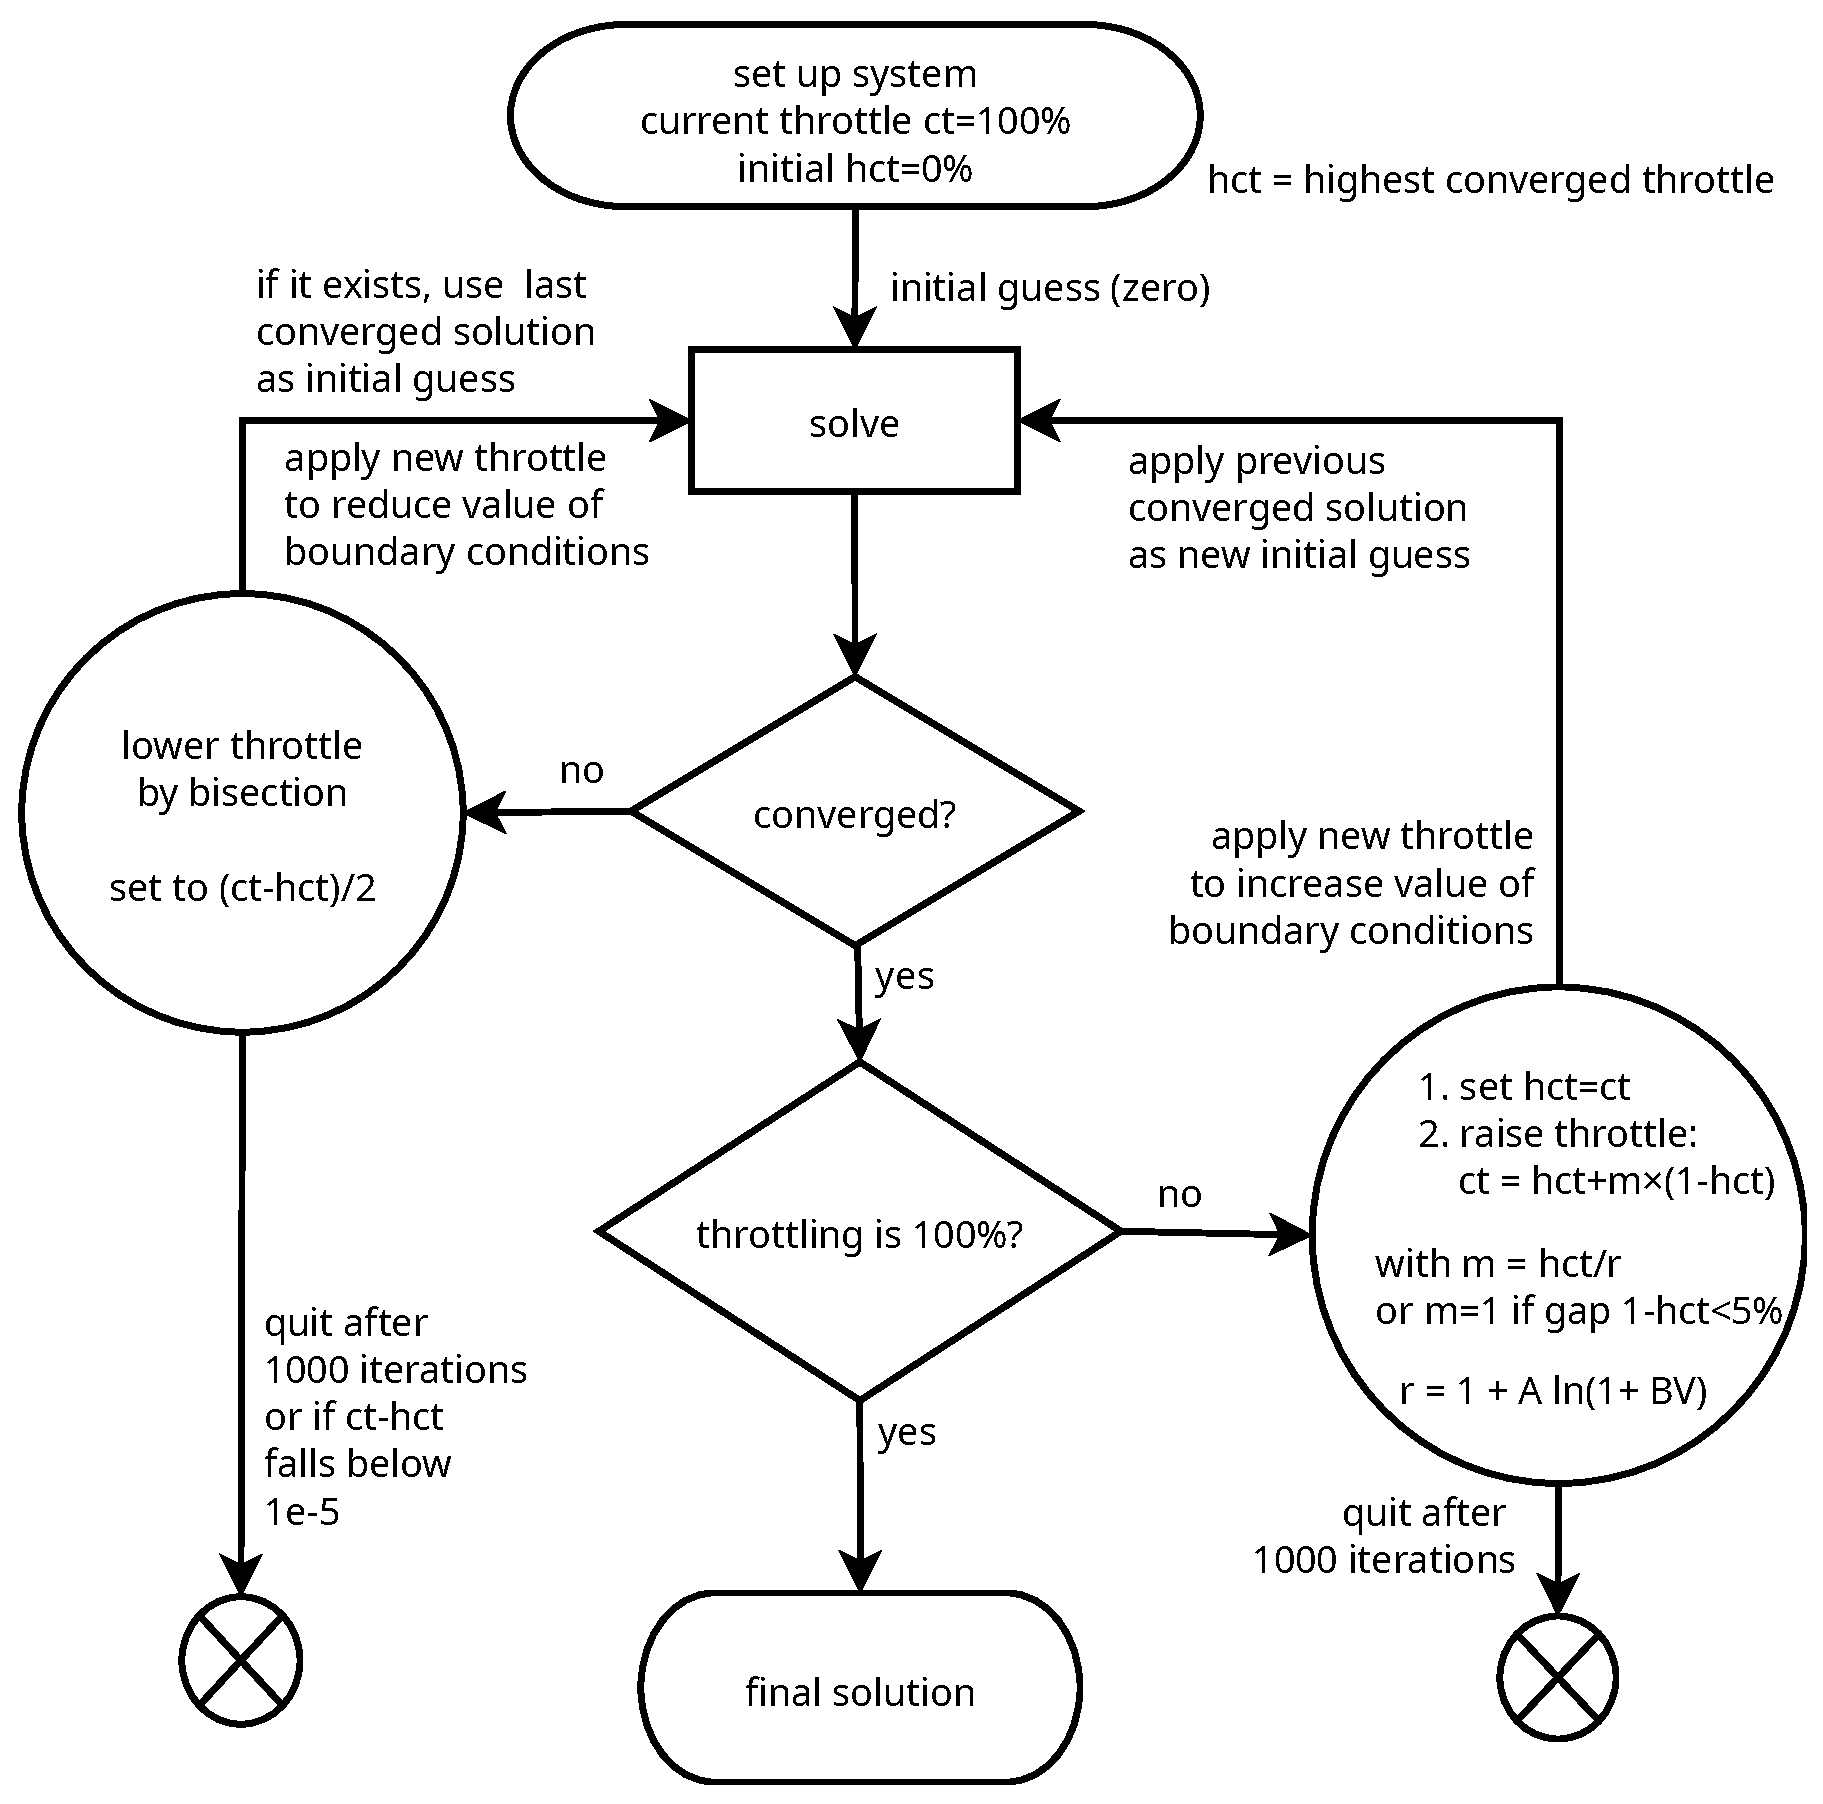
\includegraphics[width=1.1\linewidth]{throttling4.eps}
\caption{Flowchart for the throttling algorithm }
\label{fig:throttling_algorithm}
\end{figure}

The throttle is a multiplier
applied to the magnitude of the boundary conditions.
If the solver fails to converge, then we reduce the throttle downwards by
bisection between the current failed value (current throttle, ct) and the highest converged
throttle (hct, initially zero). Once the boundary
condition is throttled low enough to generate a converged solution,
we update the hct and raise
the throttle upwards by an amount $u$, closing the gap towards 100\% (we set the throttle
to 100\% if the procedure would exceed it).  The value of $u$
must find a balance between reaching a 100\% throttle in as few
iterations as possible (do not make $u$ too small), while not collapsing back to non-converging
conditions when raising the throttle (do not make $u$ too
large). Empirically, we find that, when the hct is small, the rise rate
must also be small to obtain the next converged iteration. Once the hct is
large, the rise rate may be proportionally larger. We therefore
propose a rise step $u=m\times (1- \mathrm{hct})$ such that the next
throttle applied after a converged iteration is
\begin{equation}
  \mathrm{ct [new]} = \mathrm{hct} + m (1-\mathrm{hct}),
\end{equation}
with
\begin{equation}
  m=
  \begin{dcases}
    \frac{\mathrm{hct}}{r} &, \\
    1 & \text{if } 1-\mathrm{hct} < 5\%.
  \end{dcases}
\end{equation}
This produces a quadratically accelerating rise rate and attempts a
direct jump to 100\% once the remaining gap is less than 5\%.  It is likely
that our formulation, quadratic in the hct term, approximates a more 
optimal exponential (or
sigmoidal) rise rate.

\subsubsection{Optimal Throttling}
An example of
the throttle rate against the number of iterations is presented in
Fig.~\ref{fig:throttle_rate} for 1 V and 10 V boundaries with different
choices of fixed values of the rise rate multiplier $r$. A best value of $r$ can be identified
for each voltage, minimizing the number of iterations required,
for example, $r=2$ for 1 V and $r=3$ for 10 V. A
value of $r$ larger than the best value means the rise step is
smaller, such that convergence is smooth, but requires more
iterations. A lower value of $r$ means the rise step is too large,
overstepping and resulting in a nonconverging iteration, such that
more iterations are required to fall back to a converging throttle rate.

\begin{figure}
\centering
(a)
\includegraphics[width=0.45\linewidth]{test_1V.eps}
(b)
\includegraphics[width=0.45\linewidth]{test_10V.eps}
\caption{Attempted throttle rate versus iteration numbers for (a) 1 V and
  (b) 10 V  boundaries with fixed rise rate multipliers $r=1,2,3$, and
  4. The steric model is solved with log-zero scaling.
}
\label{fig:throttle_rate}
\end{figure}

The best-performing fixed values of $r$  for potentials up to 100 V are presented 
in  Fig.~\ref{fig:best_throttle_rate}.  We observe a similar trend in 1D calculations with
trivial and log-zero function scaling  (the
differences may not be significant, since only integer values of $r$ up
to 10 were tested). A priori, we have no reason to expect the
optimal value of $r$ to be universal, and we might expect it to vary with
conditions such as the electrolyte concentration or
dimensionality. However, we plot the best $r$ values for trivial
scaling over a wide range of concentrations (1D calculations), as well as  2D and 3D calculations of the flat electrode (at a 1M
concentration). In all cases, the best $r(V)$  essentially follows the
same curve, with a small deviation seen only at 1--2 V, which can be attributed simply to the
integer resolution of the simulation.  The time per iteration varies with system conditions and
dimensionality, but the optimal $r(V)$ for minimizing the number of
iterations remains the same. The optimal $r(V)$ can be considered to be universal.



\begin{figure}
\centering
\includegraphics[width=0.8\linewidth]{best_r_vs_V.eps}
\caption{Best fixed rate multiplier $r$ for each voltage, with the lowest
  number of throttling iterations. The steric model is solved with both
  trivial (in black) and log-zero (orange dashed line) concentration scaling (1D calculation at a 1M
  electrolyte concentration).
  We also show the best $r$ values for 1D calculations with trivial scaling over a range of
  concentrations (blue stars)
  and 2D and 3D calculations (black boxes) of a flat electrode at
  a 1M concentration. The solid purple line denotes the model $r(V) = 1 +
  3.78 \ln(1 + 0.102 V)$ fitted to trivial scaling data. The grey lines
  mark uncertainty bounds of one standard deviation in the fitted parameters.
}
\label{fig:best_throttle_rate}
\end{figure}

\subsubsection{Adaptive Throttle Rate}
The trend in the best-performing $r$ values shown in Fig.~\ref{fig:best_throttle_rate} suggests that an
optimal multiplier follows
$r \propto \ln V$, indicating that $r$ 
may be tuned adaptively to provide the maximum possible rise rate (smallest
possible $r$) that minimizes the number of unsuccessful non-converged
attempts for the given boundary condition.  A milder
rise rate (larger $r$) is required at larger surface potentials.
Allowing for a finite value of $r$ when $V \rightarrow 0$, we propose
an adaptive definition of $r$,
\begin{equation}
  r(V) = 1 + A \ln(1 + B V).
  \label{adaptive_r}
\end{equation}
This model imposes the limit $r \rightarrow 1$ as $V \rightarrow 0$.
In principle, an optimal low-voltage multiplier might allow $r<1$ if
$r>$hct, but the limit of one is simpler, avoiding the need to 
compare against the hct. Fitting against the best $r$ values for trivial scaling
results in $A=3.78 \pm 0.36$ and $B=0.102 \pm 0.020 \textrm{ V}^{-1}$.
The uncertainties here have been determined from the covariance matrix
generated by the fitting procedure implemented in the
\verb|curve_fit| function provided by the \texttt{optimize} module in SciPy
\citep{VugrinSwilerRobertsStuckyMackSullivan2007}. 
 The best $r$ value for log-zero scaling is similar. One could separately fit
 parameters for log-zero scaling (to obtain 
 $A=1.3\pm 0.2$ and $B=0.7 \pm 0.5 \textrm{ V}^{-1}$).
 Nevertheless,  Fig.~\ref{fig:best_throttle_rate} shows that the
 log-zero data points lie only one standard deviation below the trivial
scaling fit. Statistically, there is no significant difference in the
best $r$ values for trivial and log-zero scaling.

We emphasize that the value of $V$ used in the adaptive $r$ formula, \eqref{adaptive_r},
must be the target boundary condition (the final electrode voltage),
and not the throttled boundary condition at the given iteration.  If a throttled $V$ were
applied, $r$ would be small when the boundary condition is strongly
throttled, resulting in large rise steps that lead to convergence
failure when the  target voltage is large.


Table~\ref{tab:convergence} shows  the number of iterations required
to converge with various boundary conditions for the different
concentration scaling functions in both the point charge model and the
steric model and applying an adaptive
$r(V)=1+3.78\ln(1+0.102V)$ for 1D meshes with 30 cells. For the point charge model, trivial scaling 
permits calculations only up to 0.7 V. Log scaling permits calculations up to 0.8 V, and log-zero
scaling permits calculations up to 1 V (1.5 V can be reached with a finer mesh).

\begin{table}
  \centering
  \begin{tabular}{c|ccc|ccc}
Pot. (V)  & \multicolumn{3}{c|}{Point Charge} & \multicolumn{3}{c}{Steric}    \\
        & Trivial & Log & Log-Zero & Trivial & Log & Log-Zero \\ \hline
%%%%%%%%%%%%%%%%%%%%%%%%%%%%%%%%%%%%%%%%%%%%%%%%%%%%%%%%%%%%%%%%%%%%%%
%%                                                                  %%
%%  This is a LaTeX2e table fragment exported from Gnumeric.        %%
%%                                                                  %%
%%%%%%%%%%%%%%%%%%%%%%%%%%%%%%%%%%%%%%%%%%%%%%%%%%%%%%%%%%%%%%%%%%%%%%
%NaCl 1M	&	&	&	&	&	&\\
%	&pot(x)/surf\_pot + non linear geometry 	&	&	&	&	&\\
%	&Steric OFF	&Steric OFF + log	&Steric OFF + log\_zero	&Steric ON	&Steric ON + log	&Steric ON + log\_zero\\
%Surface Potential [V]	&Throttle attempts	&	&	&	&	&\\
0.1	&1	&1	&1	&1	&1	&1\\
0.5	&1	&1	&1	&1	&11	&9\\
0.7	&6	&1	&1	&1	&11	&11\\
0.8	&S	&10	&6	&6	&11	&11\\
0.9	&	&S	&8	&1	&14	&12\\
1	&	&	&7	&1	&14	&12\\
1.1	&	&	&F	&7	&14	&14\\
1.5	&	&	&	&10	&15	&15\\
2	&	&	&	&8	&19	&16\\
5	&	&	&	&18	&27	&27\\
10	&	&	&	&27	&F	&39\\
100	&	&	&	&91	&	&114\\
%250	&	&	&	&240	&	&180\\
%375	&	&	&	&355	&	&212\\
%500	&	&	&	&419	&	&230\\
%625	&	&	&	&478	&	&321\\
%750	&	&	&	&517	&	&382\\
%875	&	&	&	&551	&	&428\\
1000	&	&	&	&439	&	&369    \\
2000	&	&	&	&S	&	&762    
  \end{tabular}
\caption{\label{tab:convergence}Number of throttling iterations
  required to  solve the PB model of a 1M NaCl electrolyte solution
  for various electrode potentials and concentration scaling
  functions (trivial, log, or log-zero scaling) for both the classic point charge model and the steric
 (Carnahan--Starling) model with finite ion sizes. The adaptive rise rate
  multiplier $r(V)=1+3.78\ln(1+0.102V)$ for a 1D mesh with 30 cells. 
  F = failed
  (throttle step $<10^{-5}$), and S = stopped at 1,000 iterations.}
\end{table}


Trivial scaling is successful for the steric model up to 1,000 V, while simple log
scaling fails at 10 V due to instability introduced by near-zero coion
concentrations.
Log-zero scaling enables calculations to 2,000 V
and higher, beyond the limit of trivial scaling.
The corresponding
performance plot of iterations versus voltage for the steric model
(with both trivial and log-zero scaling) is presented in Fig.~\ref{fig:convergence}.
 The steric model
naturally keeps concentrations within 
physically reasonable bounds, such that  log-zero scaling is not
required for normal electrochemical conditions. 
Trivial scaling performs better than log-zero scaling when $V<100$ V,
the region of electrochemical interest.
Performance is robust with respect to the $A$ and $B$ parameters used to
determined $r(V)$, whether fitted to the best $r$ for trivial or log-zero scaling.
2D and 3D calculations generally require the same number of iterations
as 1D calculations, showing small differences only at 1--2 V.
Even with log-zero scaling, computation of the interaction of
100 kV electrical transmission cables with saline water would require
such a large number of iterations that this algorithm would become impractical.

\begin{figure}
\centering
\includegraphics[width=0.8\linewidth]{num_attempts_vs_V.eps}
\caption{Number of throttling iterations, as a function of electrode
  voltage, needed to solve the steric model with trivial and log-zero scaling.  An adaptive rise rate multiplier
  $r(V)=1+3.78\ln(1+0.102V)$ is used to best fit trivial scaling (solid
  lines). 1D calculations with trivial scaling are shown in black,
  and log-zero scaling in orange. The rise rate $r(V)=1+1.3 \ln(1+0.7V)$
  (fitted for the best log-zero value) is also shown (dashed lines) for
  comparison. 2D data points are indicated by squares (trivial scaling) and
  diamonds (log-zero scaling). 3D data points (trivial scaling) are
  denoted by blue crosses.
}
\label{fig:convergence}
\end{figure}


The sample results of the adaptive throttling algorithm for an electrode charged to
10 V with Carnahan--Starling steric forces are presented in
Fig.~\ref{fig_results_throttling}, calculated with trivial scaling of the
concentration functions with adaptive $r$ coefficients $A=3.78$ and $B=0.102 \textrm{ V}^{-1}$).
Figure~\ref{fig_results_throttling}(b) shows the onset
of a steric adsorption layer \citep{DagmawiParsons2022} with counterion
concentrations constrained below a concentration cap determined by the
ion size, a cap of 46 mol/L in the case of our {Cl}$^{-}$ ion.

\begin{figure}
\centering
(a)
\includegraphics[width=0.45\linewidth]{steric_potential_10V.eps}
(b)
\includegraphics[width=0.45\linewidth]{steric_10V_counterion.eps}
\caption{\label{fig_results_throttling}Solutions to the modified
  PB model of a 1M NaCl electrolyte solution with
  Carnahan--Starling steric forces, shown as profiles along $x$, the
  perpendicular distance from a 10 V electrode surface. (a) Electrostatic
  potential. (b) Counterion ({Cl}$^{-}$) concentration. }
\end{figure}

\section{Conclusion}

Modelling complex electrolyte solutions in electrochemical conditions
with electrode potentials of 1 V or greater requires both nontrivial
physics and nontrivial numerical algorithms.
With respect to the
physics, aside from redox chemistry and electrolysis (not considered
here), the finite sizes of ions must be considered via
steric forces. These are expressed as a steric contribution to the
chemical potential of ions and used in the underlying thermodynamic
energy functional that provides the origin of the weak and strong
formulations of the system.
To achieve numerical convergence, we propose two
steps. First, we propose log-zero function scaling of
concentration functions that accounts
not only for the heightened concentrations of counterions near an
electrode, but also the near-zero concentrations of coions. Second and more importantly, we propose an adaptive throttling algorithm (a kind of homotopy
method) that reduces boundary conditions 
down to the linear regime, where a solution is easily obtained, and then
progressively propagates that solution by releasing the throttle
until the target boundary condition is obtained. Optimized convergence
is obtained by adaptively controlling the rise rate of the throttle factor
depending on the target boundary condition.

The combination of
log-zero scaling and throttling facilitates calculations of point
charge models up to 2 V. Log-zero scaling enables
the steric model to reach electrode potentials greater than 2,000 V. However, for typical electrochemical applications with potentials lower than 20 V,
where steric forces are needed to maintain the physical relevance
of the model, trivial scaling is sufficient and faster than log-zero scaling.
The empirical parameters for optimal throttling, minimizing the number of
required iterations, appear to be universal, independent of
the electrolyte concentration or whether the geometry is 1D, 2D, or 3D.
This might indicate a deeper structure in the algorithm that could be
revealed with further mathematical analysis. Our 1D, 2D, and 3D
simulations tested the same flat electrode surface. We expect the optimal throttling
conditions will continue to be valid with more complex 3D or 2D
geometries, though it may be prudent to confirm this assumption.

We illustrated the throttling algorithm using Dirichlet boundary
conditions (electrode potentials), but the  principle applies
equally to Neumann and more complex boundary conditions.

\begin{acknowledgement}
  We acknowledge the support of a CINECA award under the ISCRA
  initiative, for the availability of high-performance computing
  resources and support.

  A Python script demonstrating the throttle algorithm is available on Zenodo at \url{https://doi.org/10.5281/zenodo.14829963}.

\end{acknowledgement}

\bibliographystyle{spbasic}
% Write the full path of your bibfile relative to book.tex
\bibliography{chapters/parsons/bibliography.bib}


\backmatter%%%%%%%%%%%%%%%%%%%%%%%%%%%%%%%%%%%%%%%%%%%%%%%%%%%%%%%
\appendix
%\include{appendix}
% --- Matrices and vector definitions ---
\renewcommand{\vec}[1]{\bm{\mathrm{#1}}}
\newcommand{\vecGreek}[1]{\bm{#1}}
\newcommand{\mat}[1]{\bm{\mathrm{#1}}}
\newcommand{\matGreek}[1]{\bm{#1}}

% --- The defined symbols ---
\newcommand{\sbReference}{0}
\newcommand{\sbReferenceSolid}{0\solid}
\newcommand{\spPhase}{\phase}
\newcommand{\spPhaseReal}{\phase\mathrm{R}}
\newcommand{\sbPhase}{\phase}
\newcommand{\spDimension}{d}
\newcommand{\sbElemental}{e}
\newcommand{\spFluid}{\fluid}
\newcommand{\spFluidReal}{\fluid\mathrm{R}}
\newcommand{\sbFluid}{\fluid}
\newcommand{\spDiscrete}{h}
\newcommand{\spEqlb}{\mathrm{R}}
\newcommand{\spSolid}{\solid}
\newcommand{\spSolidExtra}{\solid\mathrm{E}}
\newcommand{\spSolidReal}{\solid\mathrm{R}}
\newcommand{\sbSolid}{\solid}
\newcommand{\gdim}{d}
\newcommand{\elmt}{e}
\newcommand{\h}{h}
\newcommand{\eqlb}{\mathrm{R}}
\newcommand{\defCauchyGreenRight}{\mat{C}}
\newcommand{\strainGreenLagrange}{\mat{E}}
\newcommand{\YoungsMod}{\mathrm{E}}
\newcommand{\DefGrad}{\mat{F}}
\newcommand{\stressPKi}{\mat{P}}
\newcommand{\stressPKii}{\mat{S}}
\newcommand{\xRef}{\vec{X}}
\newcommand{\xCur}{\vec{x}}
\newcommand{\CsbS}{\mat{C}_{\solid}}
\newcommand{\EsbS}{\mat{E}_{\solid}}
\newcommand{\YoungsModspS}{\mathrm{E}^{\solid}}
\newcommand{\FsbS}{\mat{F}_{\solid}}
\newcommand{\PispS}{\mat{P}^{\solid}}
\newcommand{\PispSE}{\mat{P}^{\solid\mathrm{E}}}
\newcommand{\PispF}{\mat{P}^{\fluid}}
\newcommand{\PiispS}{\mat{S}^{\solid}}
\newcommand{\PiispSE}{\mat{S}^{\solid\mathrm{E}}}
\newcommand{\PiispF}{\mat{S}^{\fluid}}
\newcommand{\XsbPhase}{\vec{X}_{\phase}}
\newcommand{\XsbS}{\vec{X}_{\solid}}
\newcommand{\XsbF}{\vec{X}_{\fluid}}
\newcommand{\xsbPhase}{\vec{x}_{\phase}}
\newcommand{\xsbS}{\vec{x}_{\solid}}
\newcommand{\xsbF}{\vec{x}_{\fluid}}
\newcommand{\strainGreenLagrangeLin}{\matGreek{\varepsilon}}
\newcommand{\Lamei}{\lambda}
\newcommand{\Lameii}{\mu}
\newcommand{\PoissonsRatio}{\nu}
\newcommand{\stressPKLin}{\matGreek{\sigma}}
\newcommand{\LinEsbS}{\matGreek{\varepsilon}_{\solid}}
\newcommand{\lispS}{\lambda^{\solid}}
\newcommand{\liispS}{\mu^{\solid}}
\newcommand{\nuspS}{\nu^{\solid}}
\newcommand{\LinPKspS}{\matGreek{\sigma}^{\solid}}
\newcommand{\LinPKspSE}{\matGreek{\sigma}^{\solid\mathrm{E}}}
\newcommand{\LinPKspF}{\matGreek{\sigma}^{\fluid}}
\newcommand{\LinPKEqlb}{\matGreek{\sigma}^{\mathrm{R}}}
\newcommand{\LinPKEqlbH}{\matGreek{\sigma}^{\mathrm{R}}_\h}
\newcommand{\Displacement}{\vec{u}}

\printindex

%%%%%%%%%%%%%%%%%%%%%%%%%%%%%%%%%%%%%%%%%%%%%%%%%%%%%%%%%%%%%%%%%%%%%%

\end{document}

